\chapter[Synthesis Feasibility Screening and Final Candidate Validation]{Synthesis Feasibility Screening and Final Candidate Validation}\label{c:result-2}

One of the fundamental challenges in AI-assisted materials discovery is ensuring that computationally predicted materials are experimentally realizable. Section \ref{section:section5-1} introduces a two-step screening approach designed to evaluate the practical synthesis feasibility of 2D perovskites. Sections \ref{section:section5-2} present the inverse design of final candidates, integrating both targeted energy level alignment and synthesis feasibility constraints to identify experimentally viable DJ-phase perovskites.

\section{Synthesis feasibility screening}\label{section:section5-1}

\subsection{Rationale and challenges}
Synthesis feasibility is a key bottleneck in AI-assisted materials discovery, acting as the bridge between theoretical predictions and experimental realization\cite{RN409,RN521}. While previous studies have investigated the synthetic feasibility of RP perovskites\cite{RN315,RN283}, no systematic approaches have been applied to DJ perovskites. This lack of established protocols arises due to two main challenges:

\begin{enumerate}
    \item Limited exploration of diammonium spacers: Unlike RP perovskites, which utilize a wide range of monoammonium cations, DJ perovskites require diammonium cations, whose synthetic pathways remain relatively underexplored.
    \item Scarcity of negative data: The absence of well-documented failed synthesis attempts (e.g., cases forming 1D or 0D phases instead of 2D structures) makes it difficult to train predictive models using traditional machine learning approaches\cite{RN422,RN592}. 
\end{enumerate}

\begin{figure}[htbp]
    \centering
    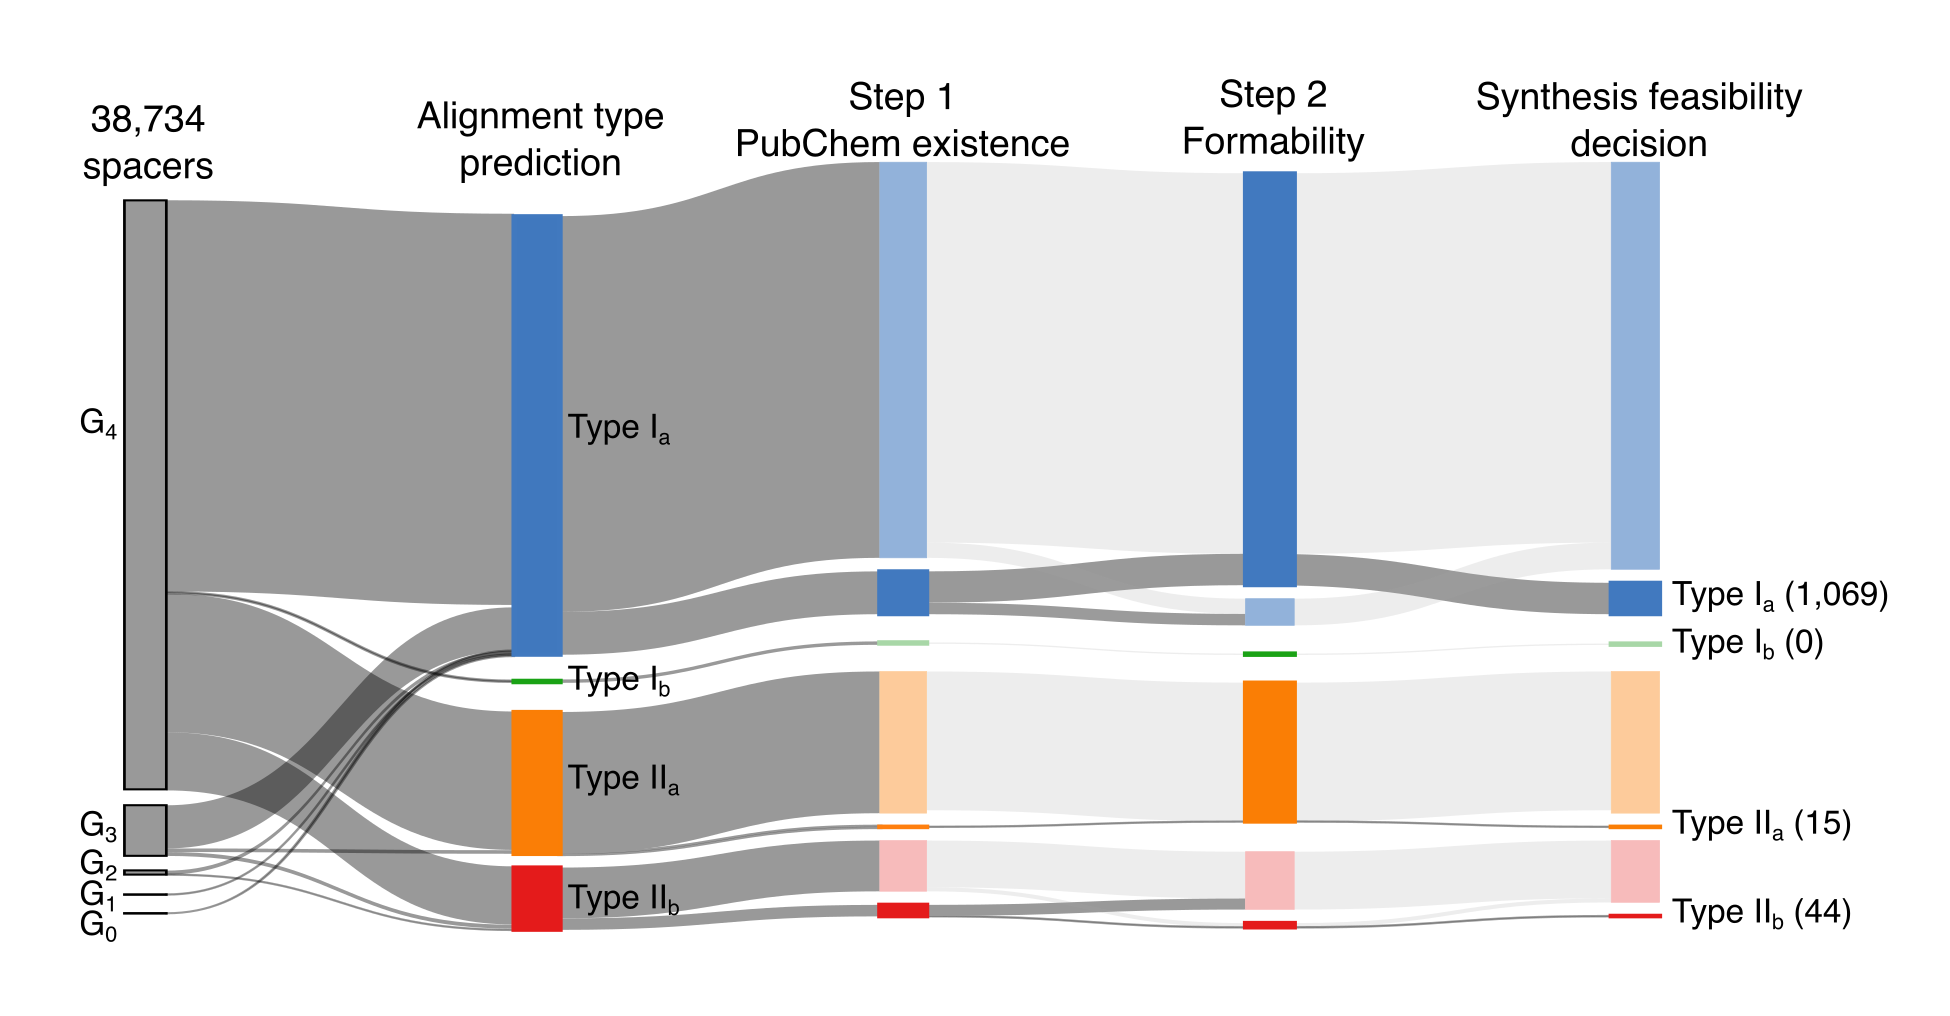
\includegraphics[width=\textwidth]{figures/synthesis-feasibility/figure5-1.png}
    \caption{Summary of synthesis feasibility screening result.}
    \label{fig:figure5.1}
\end{figure}

To address this challenge, we developed a two-step computational screening approach, mimicking the experimentalist’s approach to 2D perovskite synthesis: 

Step 1: Synthetic accessibility of organic spacers—determines whether the generated organic spacers are practically synthesizable using established chemical routes.

Step 2: Formability of 2D DJ perovskite structures—evaluate whether a given organic spacer is likely to form a stable 2D DJ perovskite phase rather than collapsing into 1D or 0D structures.

This workflow is illustrated in Figure \ref{fig:figure5.1}, with screening results shown for generations $G_0-G_4$. The following subsections provide detailed analyses of each screening step.

\subsection{Step 1: Synthetic accessibility of organic spacers}

\textbf{Using PubChem as a proxy for practical synthesizability}

\begin{figure}[htbp]
    \centering
    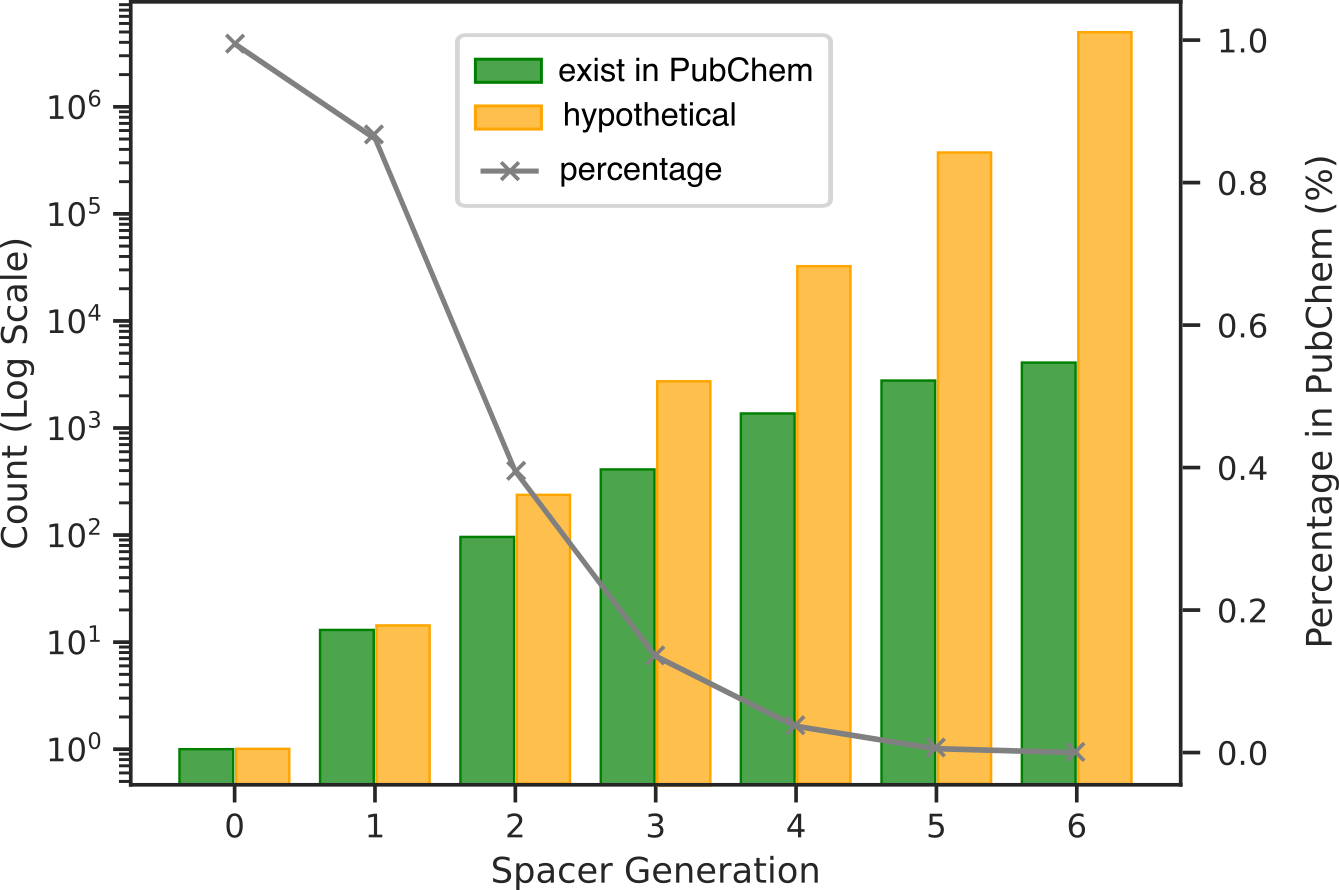
\includegraphics[width=0.7\textwidth]{figures/synthesis-feasibility/figure5-2.png}
    \caption{Number of generated organic spacers vs. existing spacers in G0-G4.}
    \label{fig:figure5.2}
\end{figure}

Rather than calculating a theoretical synthesis feasibility score, which is common in organic chemistry, we use PubChem presence as a proxy for practical synthesizability. This approach is well-established in 2D perovskite literature\cite{RN315}, as molecules listed in PubChem are generally commercially available or synthetically documented.

In our expanded chemical space ($G_0$-$G_4$), we find that 4.9\% of generated spacers are present in PubChem. The fraction of synthesizable molecules decreases progressively from $G_0$ to $G_4$ (Figure \ref{fig:figure5.2}), reflecting the increasing structural complexity of higher-generation molecules. This trend is expected since earlier generation spacers are structurally simpler and more likely to resemble known compounds, while higher-generation spacers, derived through iterative molecular morphing, tend to be chemically novel.



\textbf{Synthetic accessibility across energy level alignment types}

To determine whether synthesis feasibility is correlated with the energy level alignment type, we analysed the PubChem presence of spacers in $G_0-G_4$ with different ML-predicted energy level alignments:
\begin{itemize}
    \item Type Ib spacers present the greatest synthetic challenges, as none of them are found in PubChem.
    \item Type IIa spacers are also rare, with only 0.1\% appearing in PubChem. 
    \item Type IIb spacers are the most readily accessible, with 17.5\% present in PubChem. 
\end{itemize}

These findings suggest that certain energy alignment types are inherently more difficult to synthesize, posing additional challenges in the inverse design process.

\textbf{Structural factors affecting synthetic accessibility}

\begin{figure}[htbp]
    \centering
    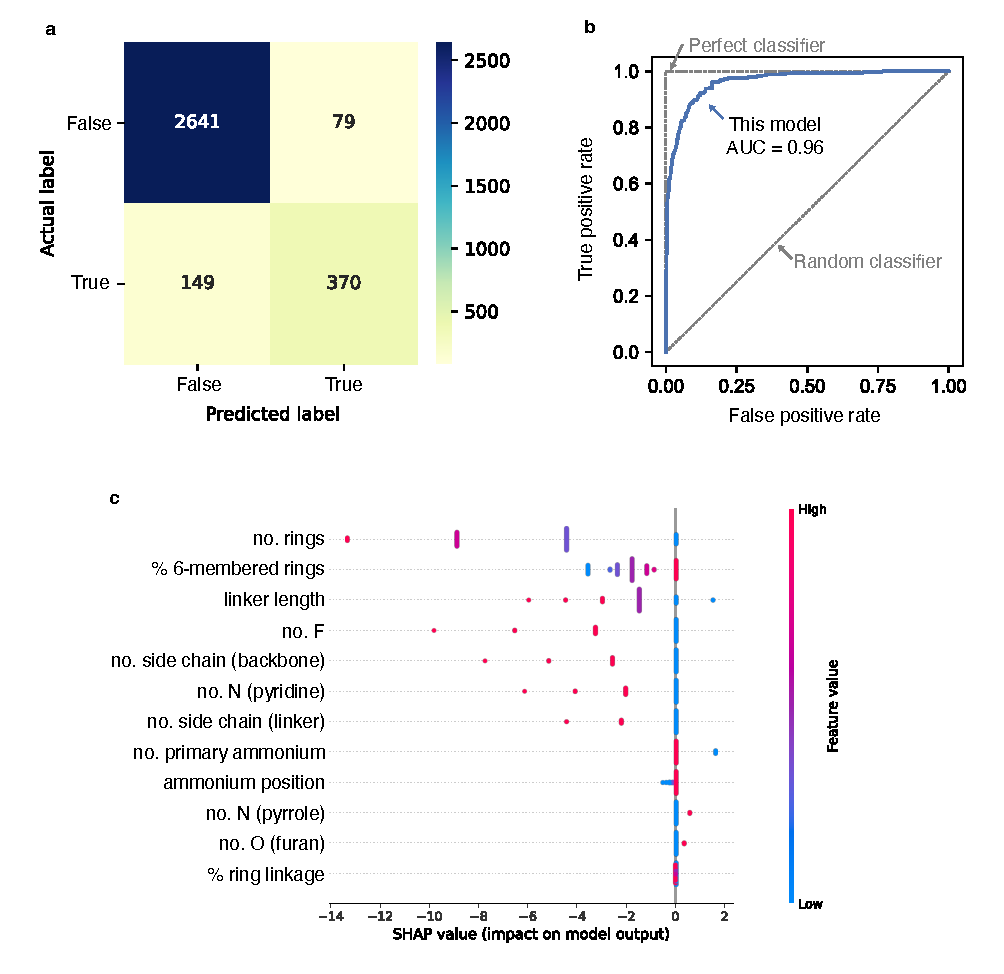
\includegraphics[width=\textwidth]{figures/synthesis-feasibility/figure5-3.pdf}
    \caption{Logistic regression analysis of the relationship between fingerprints and PubChem existence.}
    \label{fig:figure5.3}
\end{figure}

To further understand why certain molecular structures are more synthetically accessible, we trained a classification model to predict whether a given organic spacer appears in PubChem. This model follows a logistic regression framework, where:

\begin{itemize}
    \item Input Features: Molecular fingerprint descriptors.
    \item Target Property: Binary classification (exists in PubChem = 1, not in PubChem = 0).
\end{itemize}

We present the key performance metrics of the logistic regression model in Figure \ref{fig:figure5.3}. The confusion matrix (Figure \ref{fig:figure5.3}a) compares the model’s predictions with the actual labels, showing an overall accuracy of 93\%, meaning that 93\% of the total predictions were correct.

To further evaluate the model’s discriminative ability, we examine the Receiver Operating Characteristic (ROC) curve (Figure \ref{fig:figure5.3}b) and its corresponding Area Under the Curve (AUC) score. In general, a model with no discriminative power (random guessing) produces a diagonal ROC curve from (0,0) to (1,1), with an AUC of 0.5. In contrast, a perfect classifier would have a curve that rises sharply to (0,1) and extends to (1,1), corresponding to an AUC of 1.0.
Our model achieves an AUC of 0.96, with the ROC curve closely approaching the top-left corner, indicating strong predictive performance and a high degree of reliability in capturing the relationship between molecular fingerprints and synthesis feasibility.



Using SHAP value analysis, we identified key molecular features that influence synthetic accessibility (Figure \ref{fig:figure5.3}c).
The most significant descriptors include:

\begin{itemize}
    \item Number of aromatic rings: Molecules with more rings are generally less likely to be found in PubChem;
    \item Side-chain modifications: Certain branched or bulky substituents reduce synthetic accessibility;
    \item Heteroatom substitutions, especially fluorination and pyridine type nitrogen negatively impact synthesizability.
    
\end{itemize}

These findings suggest that molecular complexity—particularly higher ring counts, side chains and heteroatom substitution—tends to reduce synthetic feasibility. This aligns with general organic synthesis trends, where molecules with multiple fused rings and electronegative substitutions are often more difficult to synthesize.

By integrating PubChem data into our feasibility screening, we ensure that our selected candidates remain practically synthesizable. Although most of the identified $G_0-G_4$ spacers have not yet been explored for 2D perovskites, their presence in PubChem suggests that their chemical synthesis pathways are well established, making them promising candidates for experimental validation.

\subsection{Step 2: 2D structure formability analysis}

Following the synthetic accessibility screening, the next step evaluates the formability of 2D DJ perovskite structures. A key determinant of perovskite formability is the hydrogen-bonding interaction between the organic spacer and the inorganic framework. It has been established in the field of 2D perovskite that hydrogen bonding plays a crucial role in stabilizing 2D perovskite structures.

\textbf{Hydrogen bonding as a formability criterion}

To establish hydrogen bonding potential, we examine the interaction between donor and acceptor atoms. For a hydrogen bond to form, two conditions must be met:
\begin{enumerate}
    \item A hydrogen donor atom – A hydrogen atom covalently bonded to an electronegative element (e.g., nitrogen in ammonium groups).
    \item A hydrogen acceptor atom – A highly electronegative element, capable of accepting a hydrogen bond (e.g., halide anions (I⁻, Br⁻, Cl⁻) in the perovskite framework).
\end{enumerate}

In 2D perovskites, the halide atoms in the inorganic layers serve as hydrogen acceptors, while hydrogen-donor groups originate from the organic spacers, typically from nitrogen atom. However, not all nitrogen atoms in organic spacers are capable of forming hydrogen bonds.


\begin{figure}[htbp]
    \centering
    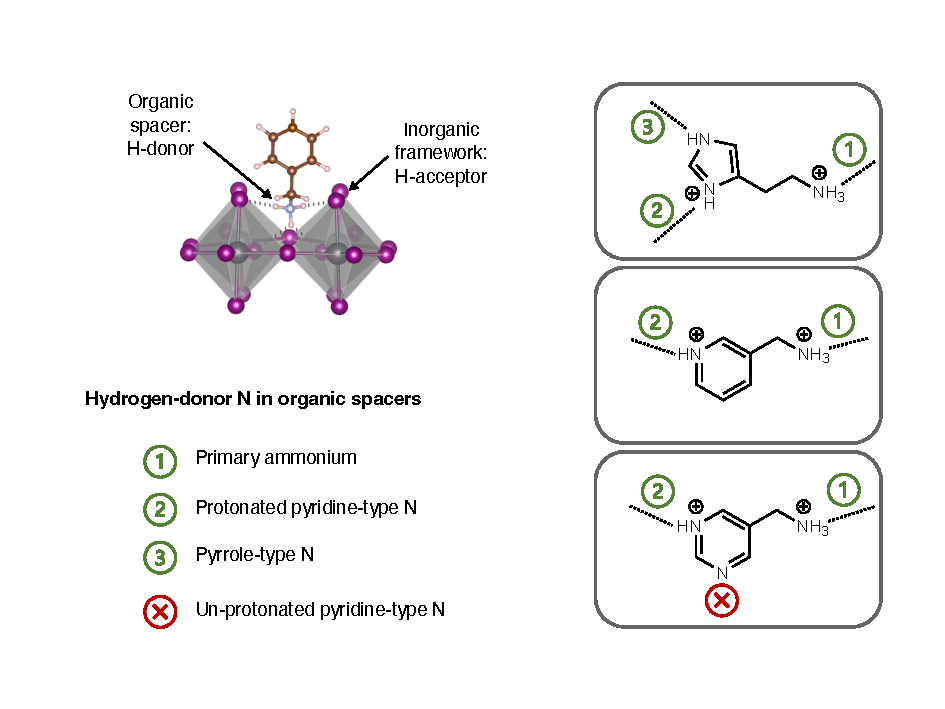
\includegraphics[width=\textwidth]{figures/synthesis-feasibility/figure5-4.pdf}
    \caption{Hydrogen-donor nitrogen for hydrogen bond formation in 2D perovskite.}
    \label{fig:figure5.4}
\end{figure}

Figure \ref{fig:figure5.4} categorizes the four nitrogen types present in the organic spacers examined in this study. Among these, only three can act as hydrogen donors:

(1) Primary ammonium ($-$NH$_3$$^+$)

(2) Protonated pyridine-type nitrogen ($-$NH$^+-$)

(3) Pyrrole-type nitrogen ($-$NH$-$)

Conversely, unprotonated pyridine-type nitrogen ($-$N$-$) cannot serve as a hydrogen donor, as it lacks a covalently bonded hydrogen. 

A few representative organic spacers containing these nitrogen types are illustrated in Figure \ref{fig:figure5.4}. For instance, in the last example, the molecule contains two pyridine-type nitrogen atoms. In its neutral form, both nitrogen atoms are equivalent, with no hydrogen bonding capability due to the absence of a covalently bonded hydrogen. However, in its charged form, if one of the nitrogen atoms becomes protonated, the additional hydrogen enables hydrogen bond formation with the inorganic framework, thereby influencing 2D structure formability.

To ensure accurate descriptor selection, our formability analysis exclusively considers hydrogen-donor nitrogen atoms while excluding non-donor types (e.g., unprotonated pyridine-type nitrogen).

\textbf{Formability descriptors}

The ability of a hydrogen-donor nitrogen to form a hydrogen bond depends not only on its presence but also on whether it can reach the inorganic framework’s halide atoms. This interaction is influenced by the topological and steric properties of the organic spacer.
To quantify these effects, we adopt four key formability descriptors, previously established in RP perovskite formability studies\cite{RN315,RN12}.

\begin{itemize}
    \item steric hindrance index (STEI) – measures spatial constraints around the hydrogen donor.
    \item eccentricity – evaluates molecular shape (ratio between height and width)
    \item nitrogen-nitrogen pair distance (Dis$_{NN}$)—Assess the spatial separation of tethering ammonium groups.
    \item the number of rotatable bonds in the spacer’s tail—Reflects molecular flexibility, influencing hydrogen bond formation.
\end{itemize}

\begin{figure}[htbp]
    \centering
    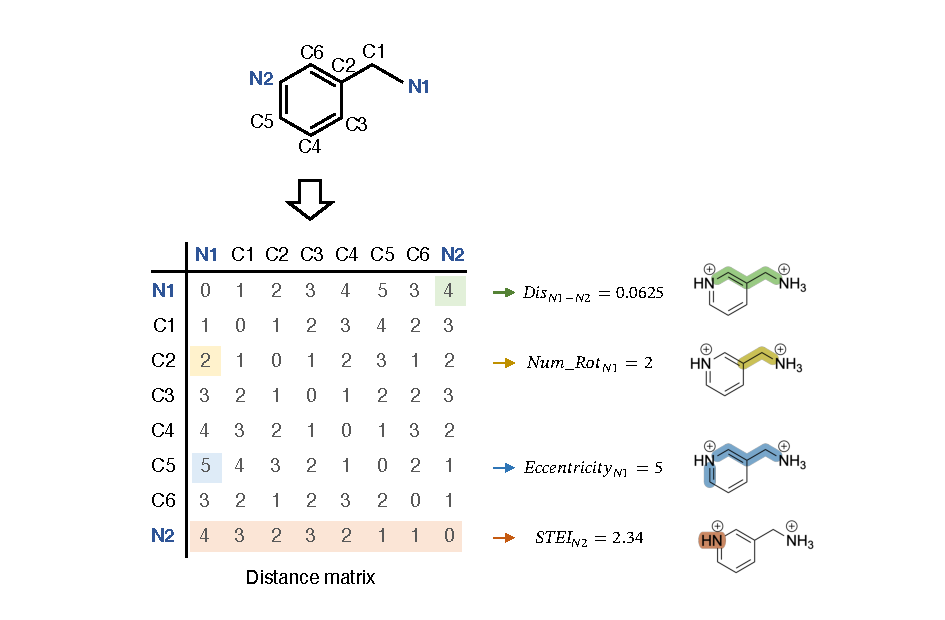
\includegraphics[width=\textwidth]{figures/synthesis-feasibility/figure5-5.pdf}
    \caption{Calculation of formability descriptors for organic spacers.}
    \label{fig:figure5.5}
\end{figure}

Each descriptor is computed using distance matrix calculations and is anchored to one or more nitrogen atoms (Figure \ref{fig:figure5.5}). Among them, Dis$_{NN}$ evaluates two nitrogen atoms, whereas the other three descriptors focus on a single nitrogen centre.

\textbf{Formability decision framework}

To access the formability of our hypothetical organic spacers, we employed a boundary-based approach, defining thresholds for each descriptor based on their physical interpretation and experimental reported positive data. 

Since prior studies suggest a linear relationship between formability and these descriptors, threshold values are determined based on the minimum or maximum range observed in experimentally validated spacers. For example, in the case of STEI, previous studies and organic chemistry principles suggest that higher steric hindrance impedes 2D perovskite formation. Thus, we set an upper limit for STEI to define formability boundaries.




\begin{figure}[htbp]
    \centering
    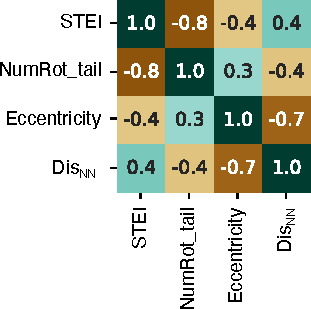
\includegraphics[width=0.4\textwidth]{figures/synthesis-feasibility/figure5-6.pdf}
    \caption{Calculation of formability descriptors for organic spacers.}
    \label{fig:figure5.6}
\end{figure}

For an organic spacer to be classified as formable, it must satisfy the boundary conditions for all four formability descriptors. Compared to machine learning classification methods commonly used in similar studies, our method addresses the unique challenge for DJ perovskites: the limitation of highly imbalanced dataset (dominated by positive data) and high correlations among descriptors which can lead to multicollinearity and reduced model accuracy. As shown by the Pearson correlation analysis of formability descriptors in Figure \ref{fig:figure5.6}, the four formability descriptors exhibit strong correlations with each other (above 0.7 for multiple descriptors), limiting their independent utility in machine learning models. Our approach applies stricter, more interpretable criteria by evaluating descriptors individually rather than collectively, enhancing its robustness for formability prediction.

\textbf{Formability screening result}

\begin{figure}[htbp]
    \centering
    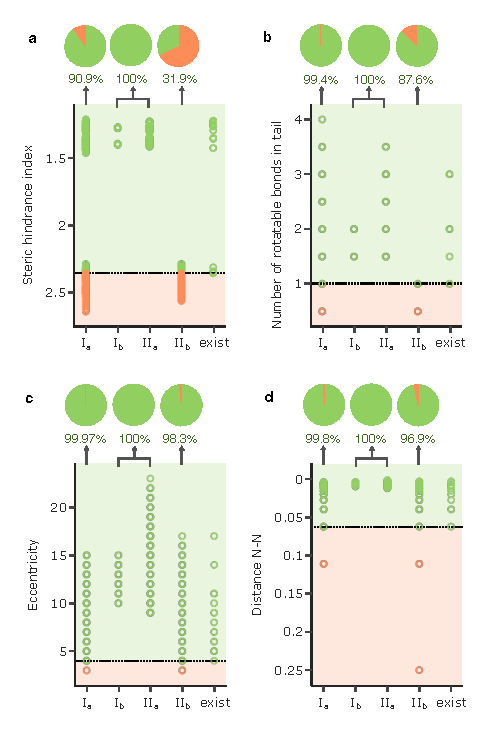
\includegraphics[width=0.8\textwidth]{figures/synthesis-feasibility/figure5-7.pdf}
    \caption{Analysis of influence of the formability descriptors on the final decision of formability.}
    \label{fig:figure5.7}
\end{figure}

Applying the formability criteria to generations $G_0-G_4$, we find that 7.4\% of organic spacers fail the screening (Figure \ref{fig:figure5.1}). However, the impact varies across energy level alignment types:
\begin{itemize}
    \item Type IIb spacers are the most affected (74\% excluded).
    \item Type Ib and Type IIa spacers are largely unaffected, with no exclusions.
\end{itemize}

The influence of the four formability descriptors on final screening decisions is also unevenly distributed. Among them, STEI exhibits the strongest impact on formability constraints. A closer examination reveals that STEI alone accounts for 68.1\% of exclusions among Type IIb spacers (Figure \ref{fig:figure5.7}). This suggests that steric effects play a dominant role in restricting the formability of these organic spacers, further reinforcing the importance of spatial accessibility in hydrogen bonding interactions within 2D DJ perovskite structures.

\begin{figure}[htbp]
    \centering
    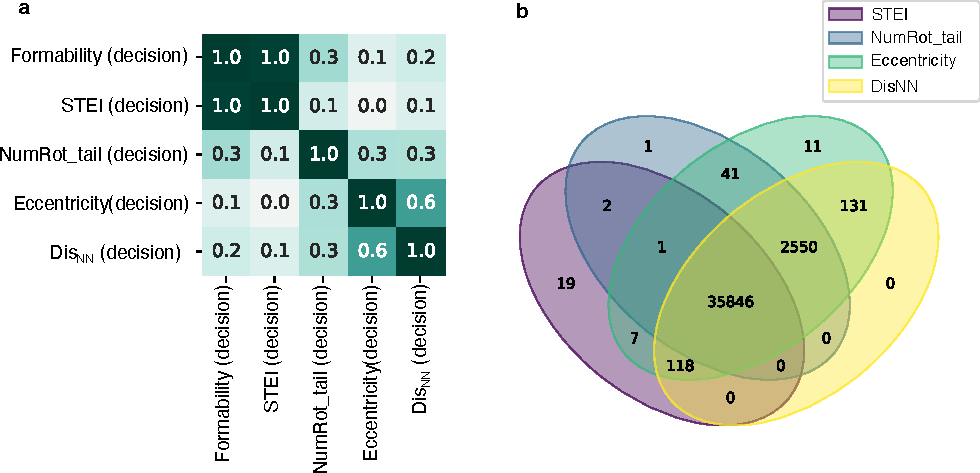
\includegraphics[width=\textwidth]{figures/synthesis-feasibility/figure5-8.pdf}
    \caption[Relationship between the decision of four formability descriptors.]{Relationship between the decision of four formability descriptors. \textbf{a} Pearson correlation coefficients between formability decisions and molecular descriptors. \textbf{b} Venn diagram illustrating the overlap in decisions among the four formability descriptors.}
    \label{fig:figure5.8}
\end{figure}

To better understand the relationship between descriptors and formability decisions, Figure \ref{fig:figure5.8}a presents a Pearson correlation analysis between the decision of individual descriptors and the final decision. The near-perfect correlation (close to 1.0) between STEI and formability confirms steric hindrance as the most critical determinant.

Additionally, Figure \ref{fig:figure5.8}b provides a Venn diagram illustrating the overlap between the decision among the four descriptors. The shared area among all four descriptors represents the organic spacers that satisfy the final formability decision criteria. Non-overlapping areas indicate that each formability descriptor serves a slightly different role in screening candidates. The largest number of candidates outside the STEI circle underscores that STEI is the most effective screening descriptor.


\textbf{Relationship between fingerprint and formability screening}

\begin{figure}[htbp]
    \centering
    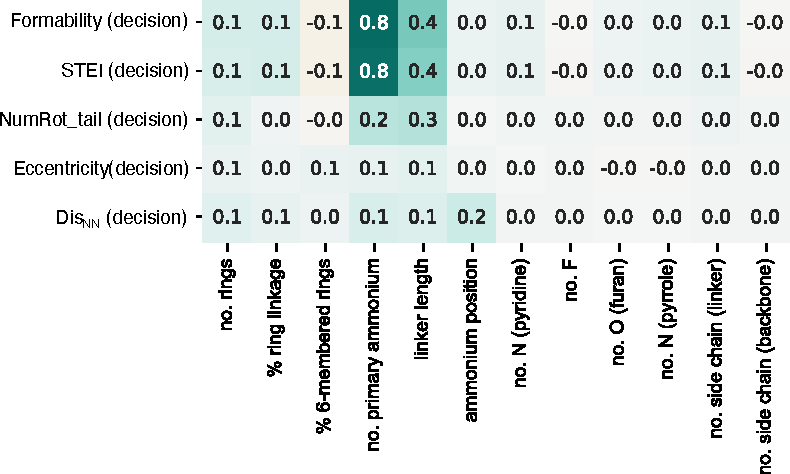
\includegraphics[width=0.8\textwidth]{figures/synthesis-feasibility/figure5-9.pdf}
    \caption{Correlation between formability descriptor decision and molecular fingerprint.}
    \label{fig:figure5.9}
\end{figure}

To further investigate the structural factors influencing 2D perovskite formability, we analysed the relationship between molecular fingerprints and formability decisions. As shown in Figure \ref{fig:figure5.9}, Pearson’s correlation coefficient reveals that key structural features affecting formability include linker length and the number of primary ammonium groups. This align with established understanding in this field\cite{RN144}, emphasizing that the tethering ammonium group plays a crucial role in the formation of 2D perovskite structure. 

The influence of the tethering ammonium group is primarily exerted through its impact on the STEI, which determines whether the ammonium donor can effectively engage in hydrogen bonding with the inorganic framework. This effect explains why Type IIb spacers are disproportionately affected by formability screening—compared to Type IIa and Type Ib spacers, Type IIb spacers exhibit shorter linker lengths and fewer primary ammonium groups, leading to increased steric hindrance and reduced hydrogen bonding potential.




Although our analysis confirms that the tethering ammonium group is the dominant factor in formability, we also observe weaker correlations between formability and other structural descriptors. To explore these additional dependencies, we analysed representative groups of organic spacers to illustrate that formability is governed by complex interactions between multiple structural variables.

As shown in Figure \ref{fig:figure5.10}, formability in this set of organic spacers is determined by a combination of factors: tethering ammonium position, linker length, number of primary ammoniums, and the percentage of six-membered rings. 

Among these descriptors, the rotatable bond in the tail descriptor is primarily influenced by linker length, particularly when there is a single primary ammonium, and the linker length is zero. In contrast, STEI involves a more complex interplay of factors, including the number of primary ammoniums, linker length, and ammonium position. While steric hindrance is often associated with the number of primary ammoniums, our findings reveal that this factor alone is insufficient to disqualify an organic spacer. Instead, the spatial environment of secondary ammoniums, particularly the position of the tethering ammonium on the ring, is a key determinant of the STEI boundary. 

\begin{figure}[htbp]
    \centering
    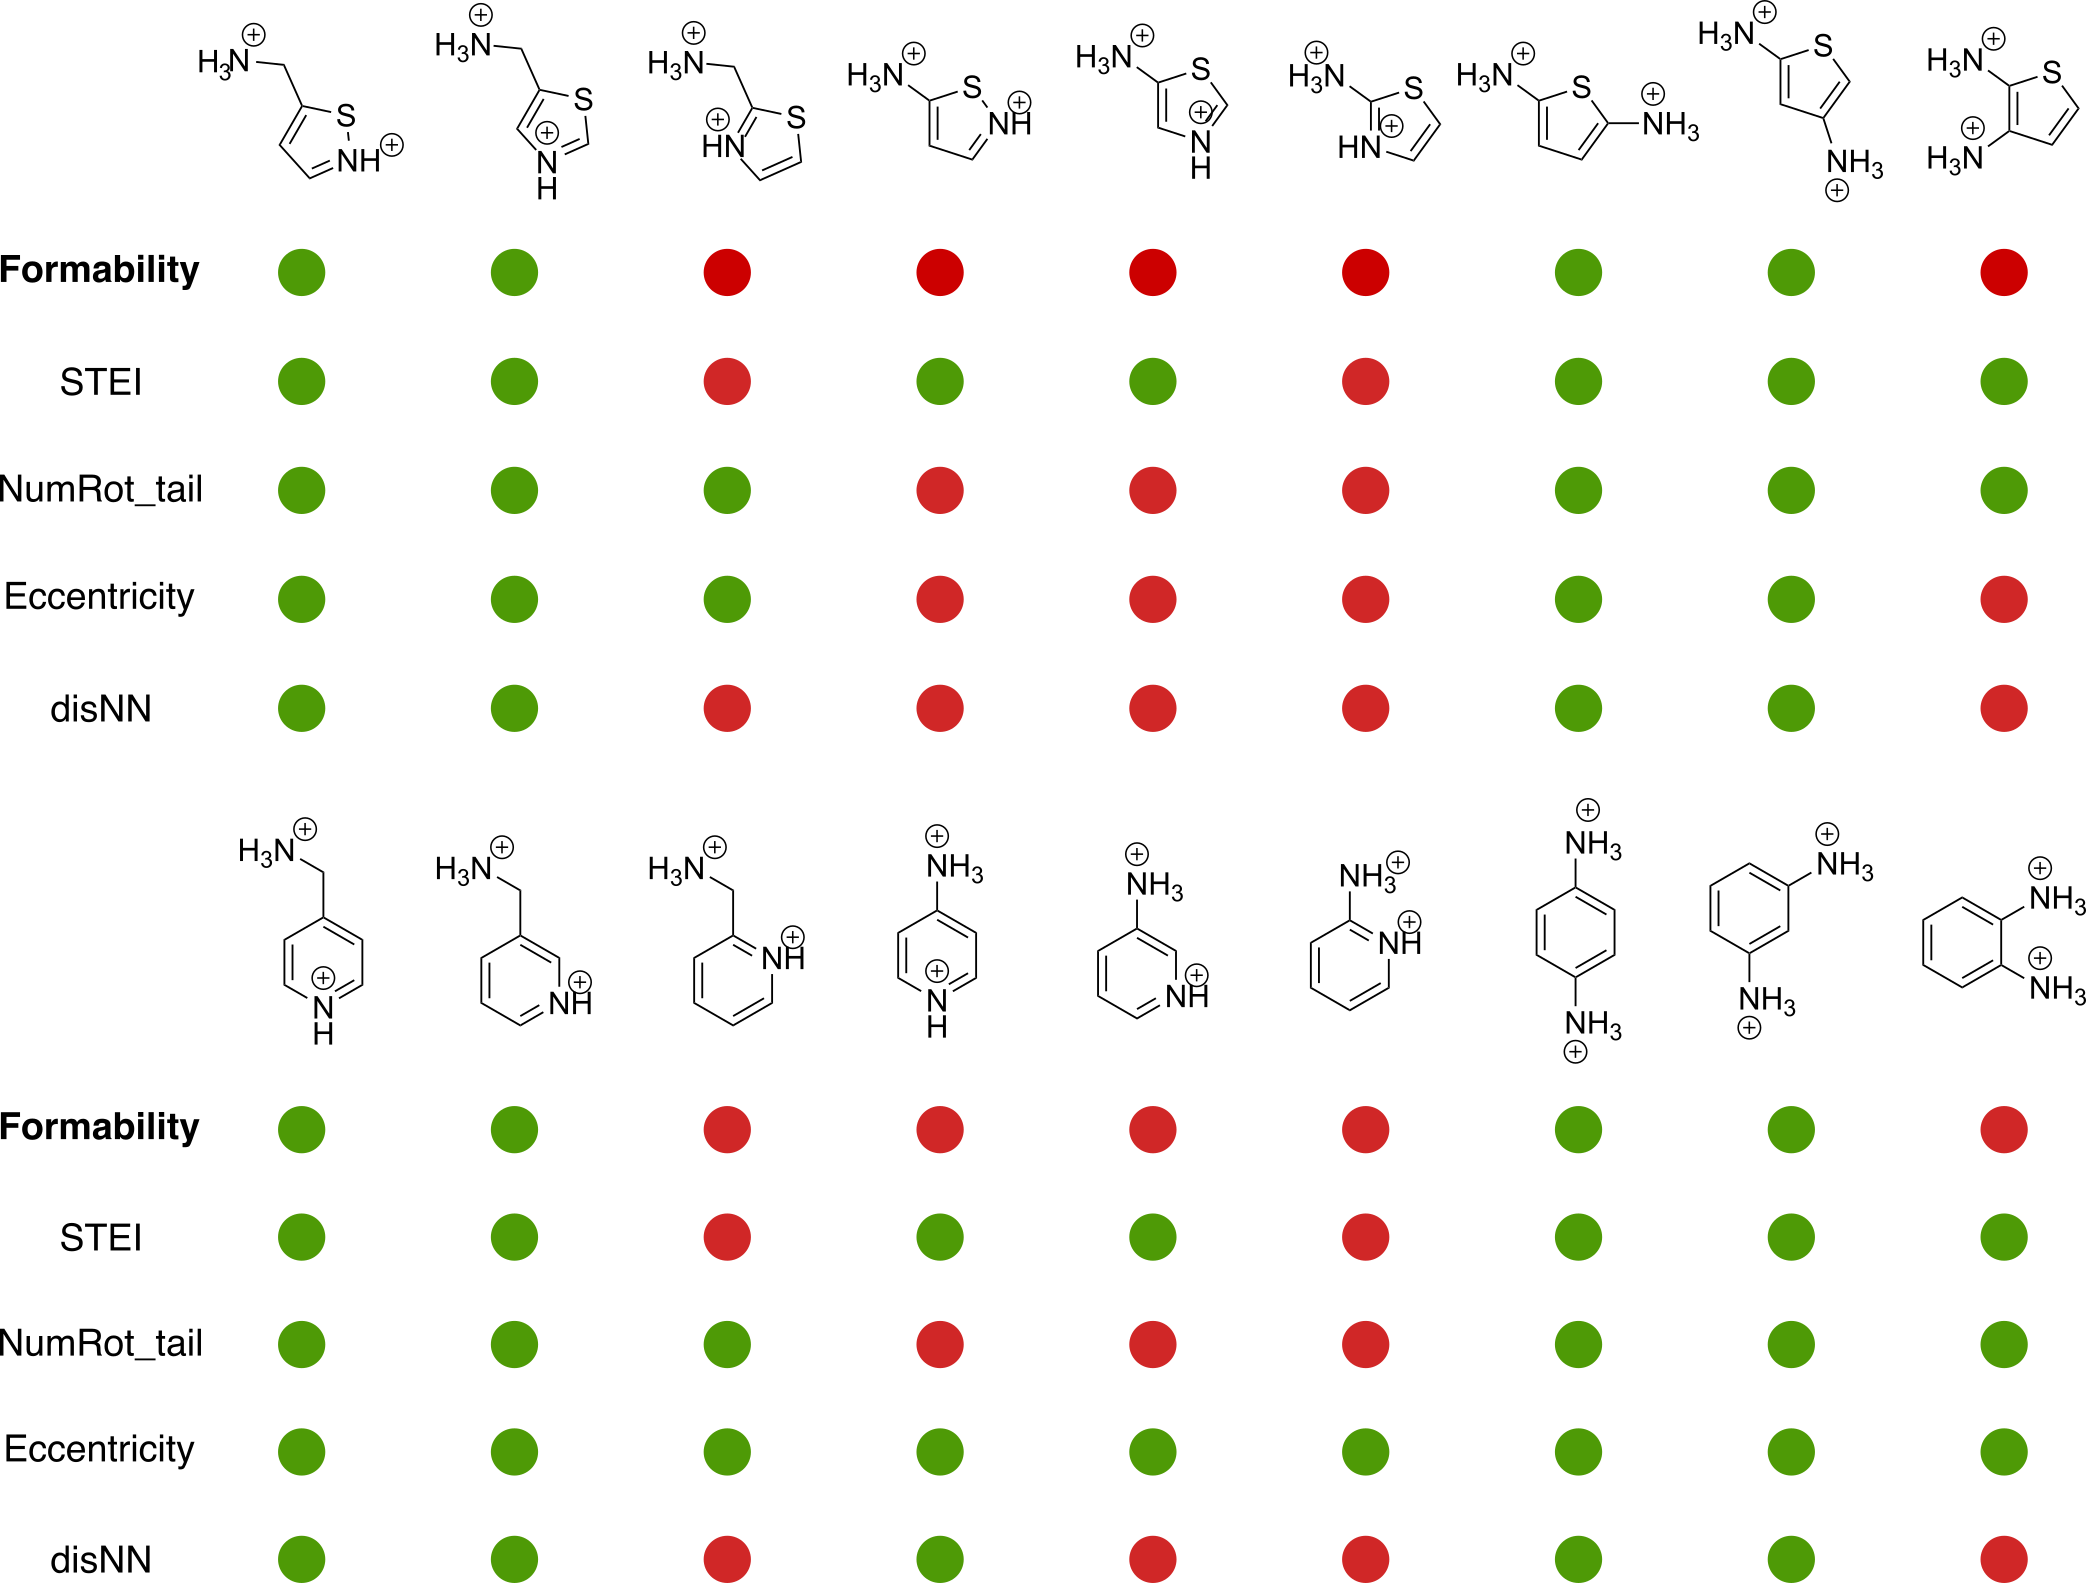
\includegraphics[width=\textwidth]{figures/synthesis-feasibility/figure5-10.png}
    \caption{Examination of similar organic spacers near the formability decision boundary. }
    \label{fig:figure5.10}
\end{figure}

\subsection{Synthesis feasibility screening summary}

Our synthesis feasibility screening reveals distinct synthesis feasibility challenges for DJ perovskites with type Ib, IIa, and IIb alignments. For type Ib and IIa organic spacers, the primary bottleneck lies in their synthetic accessibility, whereas for type IIb spacers, the main challenge is achieving the formability of the 2D structure. 

While this two-step screening process effectively narrows the range of DJ perovskite candidates, limitations remain when compared to real experimental synthesis. 
First, while PubChem provides a practical and high-throughput filter, certain organic spacers not listed in its database may still be accessible through complex synthetic routes, as demonstrated in organic photovoltaic research\cite{RN282}. 
Second, the formability descriptors rely on boundaries derived from reported positive data, leaving unexplored regions in the parameter space. Refining these boundaries as new DJ-phase spacers are reported could further expand the pool of viable candidates. 
Finally, the screening process does not fully capture certain experimental considerations critical to practical synthesis. For conjugated organic spacers, solubility stands out as a significant factor. Specifically, increasing the number of rings to three or more can lead to solubility issues\cite{RN304}, which are particularly relevant for type Ib and IIa spacers. This challenge may be mitigated by structural modifications, such as incorporating short alkyl side chains to disrupt the planarity of the conjugated backbone, a strategy commonly employed in organic photovoltaics\cite{RN282,RN619}. Additionally, key experimental parameters—such as solvent choice, precursor ratios, temperature, and pH—are not accounted for in our method. These factors can influence whether the DJ phase forms or if alternative phases (e.g., 1D, 0D, or RP phase) are favoured with the same organic spacer\cite{RN12}. 

\section{Inverse design of DJ perovskites with targeted energy level alignment}\label{section:section5-2}

In this section, we apply an inverse design strategy for selecting organic spacers that achieve three specific energy-level alignment types relevant to DJ perovskite applications: Type IIa, Type IIb, and Type Ib. This approach leverages the invertible molecular fingerprint representation, allowing us to map from desired energy level alignments back to potential organic spacer structures. First, we identify unique fingerprint characteristics based on ML-predicted energy level alignment and synthesis feasibility analysis. These fingerprints are then inverted to reconstruct the corresponding organic spacer structures within the expanded chemical space. Since the fingerprint criteria follow well-defined boundary conditions, this method enables a systematic and exhaustive exploration of the chemical space for targeted alignment types.

\subsection{Rationale for inverse design framework}

The primary objectives of our inverse design approach are:

(1)	Exploring uncharted regions of the DJ perovskite energy landscape, focusing specifically on Type IIa, Type IIb, and Type Ib alignments.

(2)	Ensuring synthetic feasibility, so that the identified organic spacers are relevant for experimental validation.

\textbf{Limitations of the forward design approach}

Up to this point, our computational design strategy has relied on a forward design approach, employing high-throughput screening to evaluate $\sim10^4$ hypothetical organic spacers. This has successfully led to experimentally viable Type IIa and Type IIb candidates. However, two critical challenges remain:

(1)	Absence of Type Ib candidates: Despite screening a large chemical space, no organic spacers satisfying Type Ib energy alignment have been identified. This is primarily due to synthetic challenges, as many potential Type Ib spacers are systematically filtered out during feasibility screening.

(2)	Limited Exploration of the Chemical Space. The screening process has been constrained to lower-generation organic spacers ($G_0-G_4$), totaling $\sim10^4$ candidates. However, the number of possible organic spacers increases exponentially in later generations. This means that a significant portion of the design space remains unexplored, potentially missing optimal organic spacers that exist beyond the current screening limits.

\textbf{Transitioning to an inverse design approach}

To overcome the limitations of forward design, we adopt an inverse design approach, leveraging our invertible molecular fingerprint representation—a key feature of our forward design workflow. This enables us to reverse-engineer organic spacer structures directly from target energy level alignments while ensuring synthetic feasibility.
Unlike forward design, which requires exhaustive screening, this inverse approach allows us to map directly from desired properties (energy level alignment and synthesis feasibility) to molecular fingerprints, and subsequently to organic spacer structures.
The inverse design process consists of the following steps:

(1)	Identify molecular fingerprints associated with targeted energy level alignments and synthetic feasibility constraints.

(2)	Reconstruct organic spacers by inverting the selected fingerprints. Obtain synthesizable candidate through synthesis feasibility screening.

(3)	Validate the energy level alignment of the designed DJ perovskites through DFT calculations.

By implementing this target-driven approach, we bypass the computational bottlenecks of exhaustive forward screening, enabling a systematic and efficient exploration of the chemical space to identify optimal organic spacers.

\subsection{Constructing fingerprint for targeted alignment types}

Previous chapters have established a strong correlation between molecular fingerprints and energy level alignment types. By analysing statistical trends in the fingerprint data from $G_0-G_4$ organic spacers, we identify distinct molecular features that are closely associated with specific alignment types.



\begin{figure}[htbp]
    \centering
    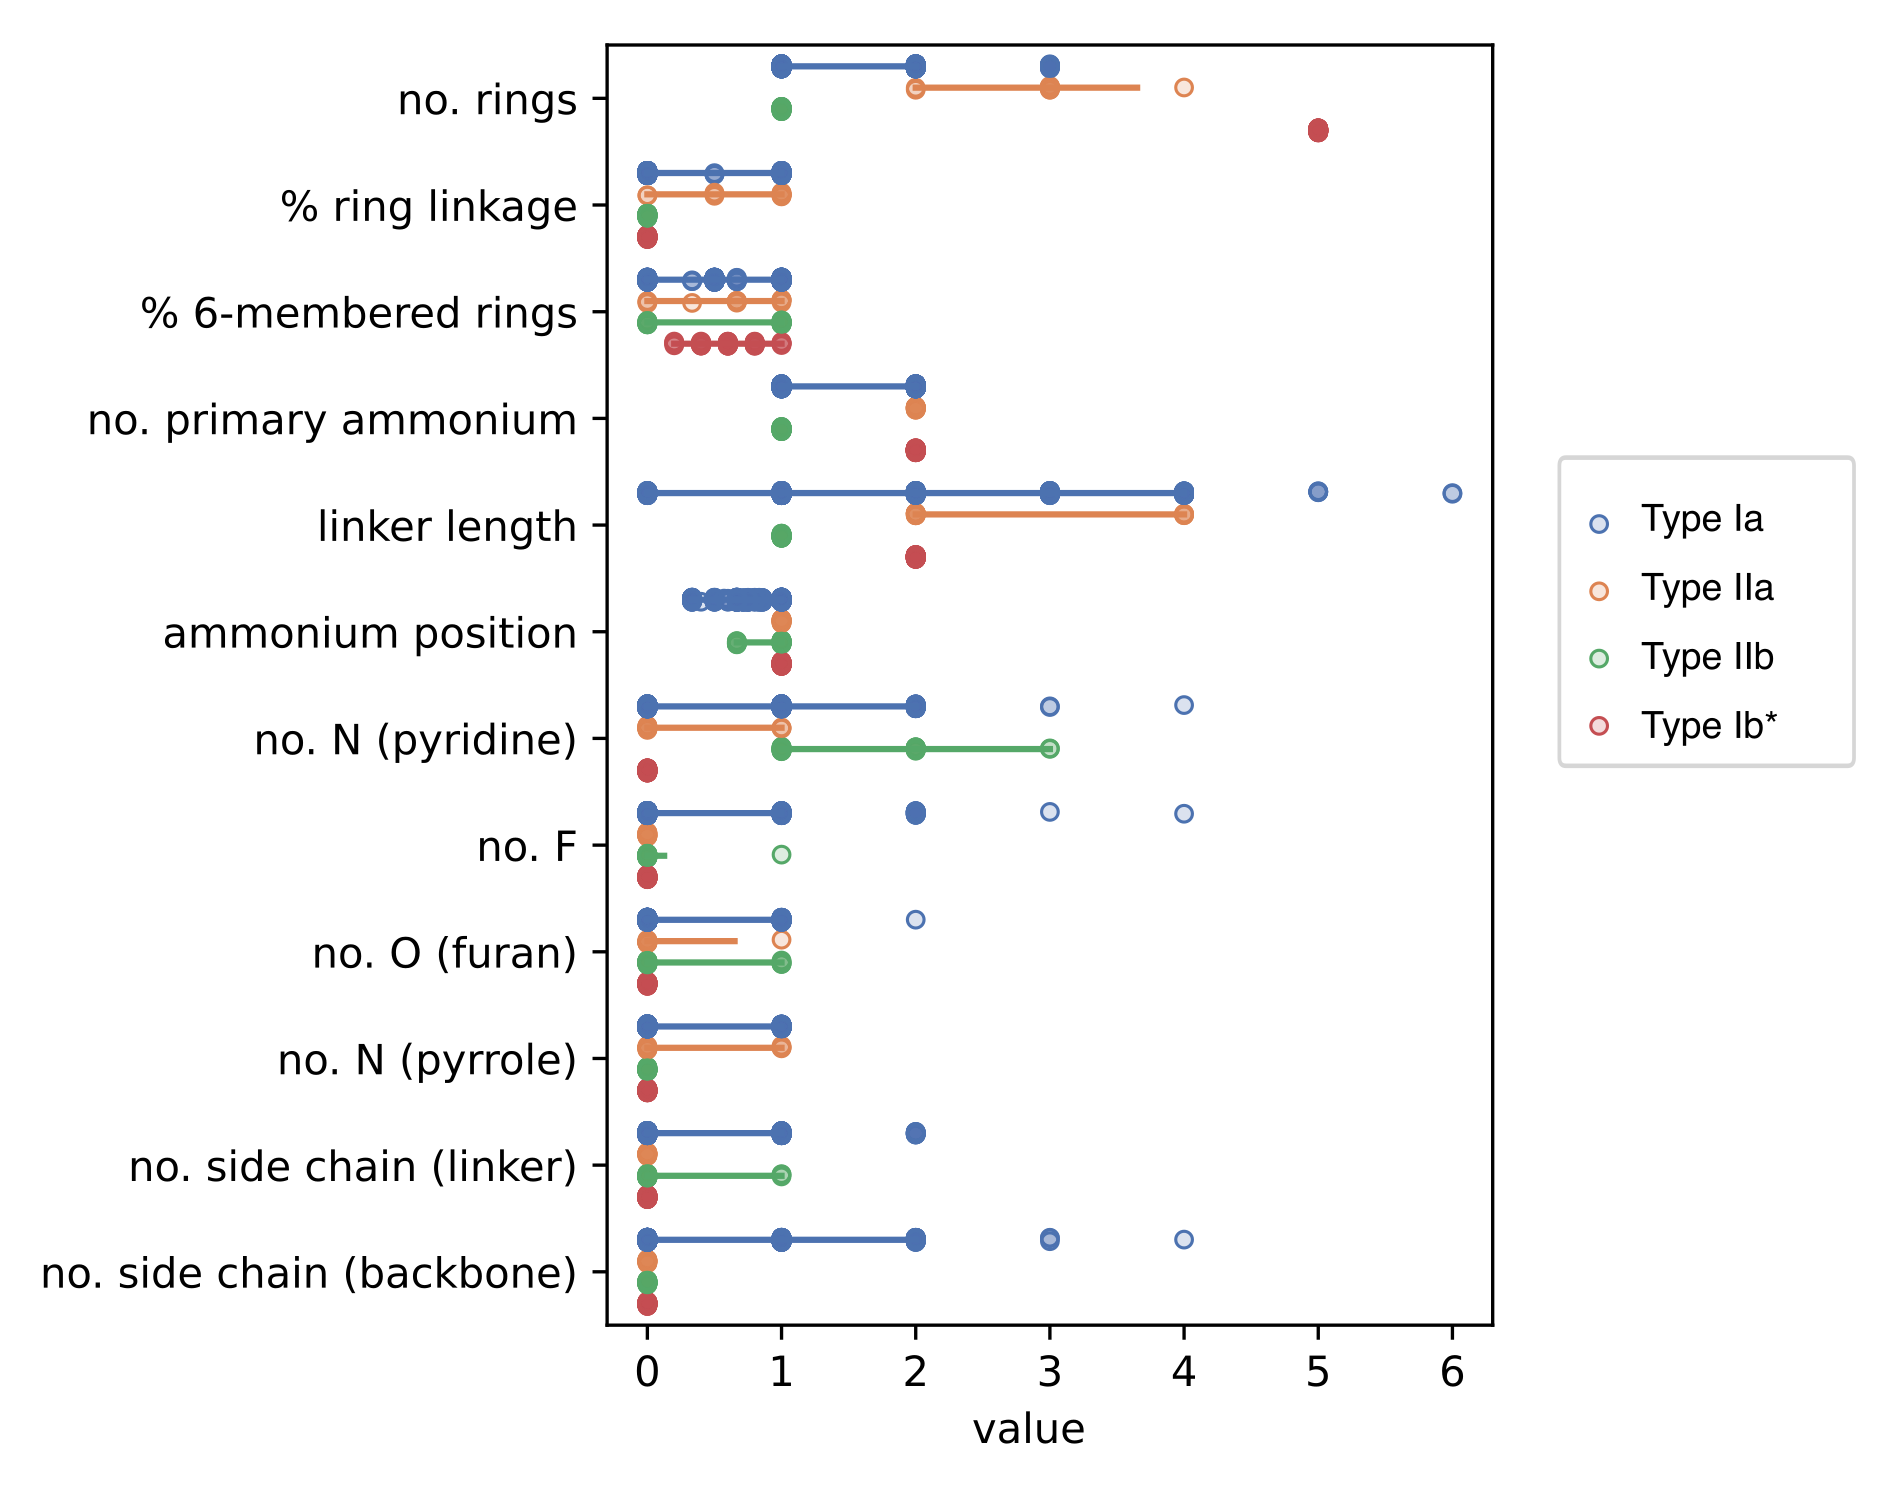
\includegraphics[width=0.9\textwidth]{figures/synthesis-feasibility/figure5-11.png}
    \caption{Distribution of organic fingerprints associated with different energy level alignment types.}
    \label{fig:figure5.11}
\end{figure}

Figure \ref{fig:figure5.11} presents the distribution of 12 molecular descriptors in organic spacers that pass synthetic feasibility screening, categorized by their respective alignment types.
The statistics of the 12 organic descriptors for qualified organic spacers from $G_0-G_4$ are depicted. The dots indicate the range, while the bars represent the 95\% confidence interval of each descriptor, color-coded according to their alignment type (Ia, IIa, IIb). For Type Ib spacers, no candidates were identified in $G_0-G_4$, primarily due to synthetic accessibility constraints. To gain insight into their characteristic features, we considered organic spacers that theoretically satisfy Type Ib energy alignment without enforcing synthetic feasibility constraints.

We identified distinct molecular fingerprint characteristics associated with different energy level alignments. Type Ia spacers exhibit a broader range of descriptor values, which corresponds to their higher prevalence in the organic spacer dataset. In contrast, Type IIa, IIb, and Ib spacers display more defined clustering patterns, suggesting that specific molecular features play a critical role in determining their alignment behaviour.

Among these, the number of rings, primary ammonium groups, and linker length emerge as the key distinguishing factors. Notably, the number of rings differs significantly across alignment types: Type Ib = 5; Type IIa = 2–4; Type IIb = 1.

These trends provide valuable insights into the molecular fingerprint characteristics most likely to yield qualified organic spacers for targeted energy level alignments.

\begin{figure}[htbp]
    \centering
    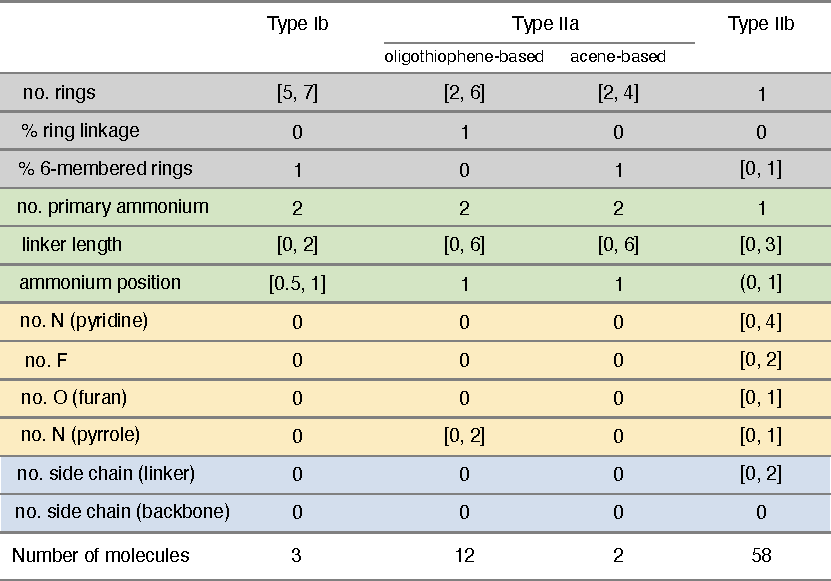
\includegraphics[width=\textwidth]{figures/synthesis-feasibility/figure5-12.pdf}
    \caption{Fingerprint criteria for targeted energy level alignment type.}
    \label{fig:figure5.12}
\end{figure}

Based on statistical probability analysis, we define boundary conditions for fingerprint values that are most likely to correspond to targeted energy level alignment types (Figure \ref{fig:figure5.12}). The fundamental principle in setting these criteria is to capture the range indicated by the confidence interval, ensuring that the selected fingerprint space is broad enough to include promising candidates while remaining computationally manageable.

For example, Type IIa spacers encompass a large number of candidates if a single fingerprint set is used. To refine the selection and improve specificity, we introduce additional fingerprint criteria based on the conjugated backbone structure. Specifically, we classify Type IIa spacers into two distinct subgroups: oligothiophene-like organic spacers, characterized by linked 5-membered rings; and acene-like organic spacers, featuring fused 6-membered rings.

By establishing fingerprint-based selection criteria, we define a finite and exhaustible chemical search space (as demonstrated below), enabling a systematic and targeted search for viable organic spacers that satisfy both energy alignment and synthetic feasibility constraints.

\textbf{Exhaustive search of chemical space}

\begin{figure}[htbp]
    \centering
    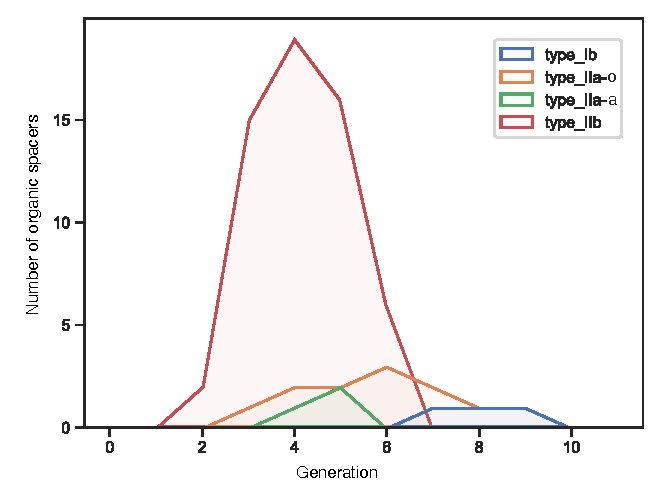
\includegraphics[width=0.8\textwidth]{figures/synthesis-feasibility/figure5-13.pdf}
    \caption{Organic spacer counts for each energy alignment type across generations $G_0-G_{11}$}
    \label{fig:figure5.13}
\end{figure}

Using the fingerprint criteria, we systematically map the chemical space to identify potential organic spacers that meet the desired energy alignment and synthesis feasibility constraints. As shown in Figure \ref{fig:figure5.13}, the number of viable organic spacers for each fingerprint criterion follows a single-peak distribution across generations: Starts at zero in early generations ($G_0-G_1$).; Peaks at an intermediate generation ($G_5-G_9$); Diminishes to zero by $G_{11}$, marking a natural endpoint where no additional spacers satisfy the criteria.
The decline at $G_{10}$ and $G_{11}$ suggests that beyond these generations, no additional chemically meaningful spacers are likely to exist within the defined fingerprint constraints.

This approach enables us to overcome the limitations of the enumerable chemical space ($G_0-G_6$, approximately $10^6$ spacers, with the number expected to increase exponentially in later generations) and conduct an exhaustive search across the entire chemical space within the defined fingerprint constraints. While viable spacers may exist beyond this subregion, our analysis suggests that it represents the most promising region for identifying candidates efficiently while maintaining an affordable computational cost. 

Our search identified three type Ib organic spacers in $G_7-G_9$, 14 type IIa candidates in $G_3-G_9$, and 58 type IIb candidates in $G_2-G_6$. 

\subsection{Mapping fingerprint to organic spacers structures}
\textbf{Type Ib}

\begin{figure}[htbp]
    \centering
    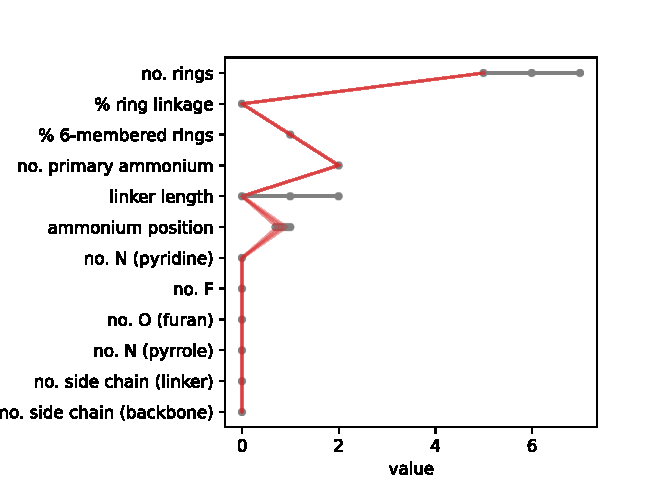
\includegraphics[width=0.8\textwidth]{figures/synthesis-feasibility/figure5-14.pdf}
    \caption{The explored fingerprint range and vs. fingerprint range of type Ib final organic spacer candidate.}
    \label{fig:figure5.14}
\end{figure}

For Type Ib alignment, the identified fingerprint range corresponds to 347 organic spacers. However, only three of these spacers pass the synthesis feasibility screening, primarily due to synthetic accessibility constraints.

The fingerprint range of the selected organic spacers is shown in Figure \ref{fig:figure5.14}. All three share highly similar fingerprint characteristics, with the only variation being ammonium position. Their key structural features include:

-	A conjugated backbone consisting of five fused 6-membered rings.

-	Two ammonium groups serving as tethering groups.

-	No heteroatom substitutions (e.g., nitrogen, oxygen, or fluorine).

-	No side chains attached to the backbone.

As illustrated by the explored range of organic fingerprints, organic spacers with additional variations—such as an increased number of rings, longer linker lengths, or alternative linker positions—were excluded from the final selection, primarily due to their absence from the PubChem database, indicating limited synthetic accessibility.

The structures of the three identified organic spacers are presented in Figure \ref{fig:figure5.15}.

\begin{figure}[htbp]
    \centering
    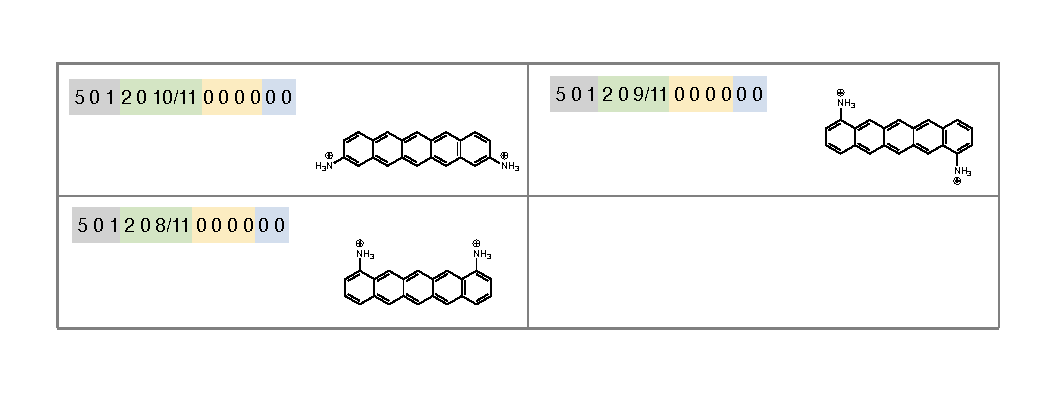
\includegraphics[width=\textwidth]{figures/synthesis-feasibility/figure5-15.pdf}
    \caption{Inverse designed candidates for type Ib alignment.}
    \label{fig:figure5.15}
\end{figure}

\textbf{Type IIa}

For Type IIa spacers, the identified fingerprint set corresponds to 720 organic spacers for oligothiophene-like structures and 88 organic spacers for acene-like structures. After applying synthesis feasibility screening, only 14 candidates remained as final selections.

\begin{figure}[htbp]
    \centering
    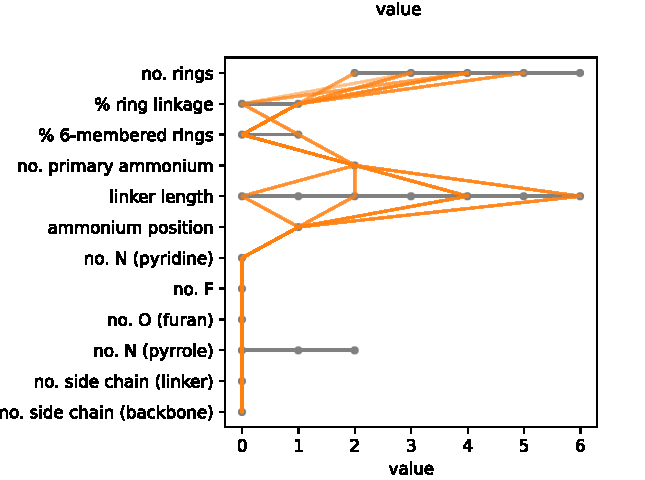
\includegraphics[width=0.8\textwidth]{figures/synthesis-feasibility/figure5-16.pdf}
    \caption{The explored fingerprint range and vs. fingerprint range of type IIa final organic spacer candidate.}
    \label{fig:figure5.16}
\end{figure}

The fingerprint range of the selected final candidates is shown in Figure \ref{fig:figure5.16}. These candidates primarily exhibit the following key structural characteristics:

-	Conjugated Backbone: Multiple linked thiophene rings (oligothiophene-like) or fused benzene rings (acene-like).

-	Tethering ammonium groups: Two primary ammonium groups with varying linker lengths.

-	No heteroatom substitutions (e.g., nitrogen, oxygen, fluorine).

-	No side chains attached to the backbone.

\begin{figure}[htbp]
    \centering
    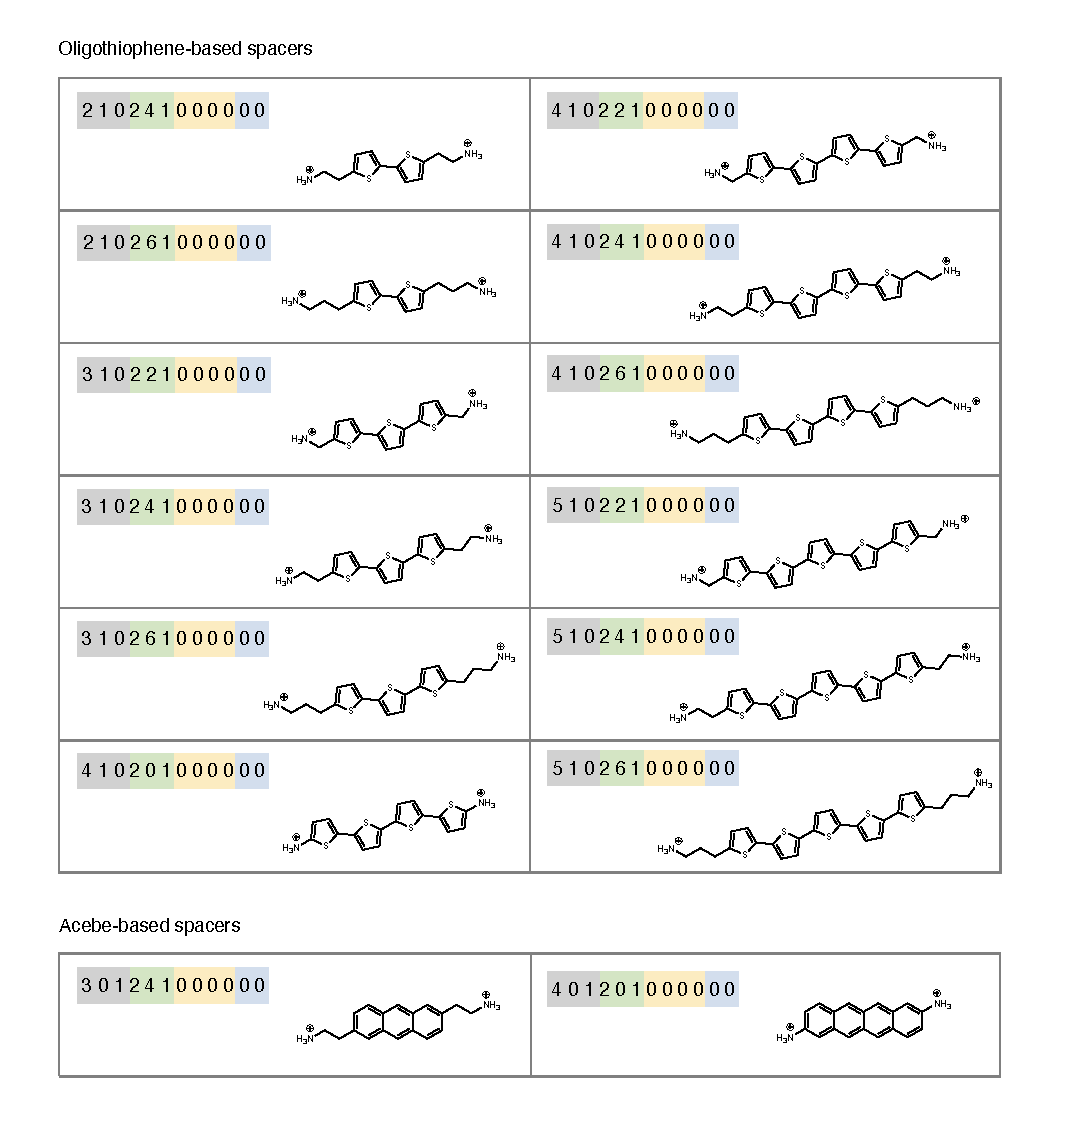
\includegraphics[width=\textwidth]{figures/synthesis-feasibility/figure5-17.pdf}
    \caption{Inversed designed candidates for type IIa alignment.}
    \label{fig:figure5.17}
\end{figure}

The organic spacer structures are presented in Figure \ref{fig:figure5.17}. Notably, for each fingerprint, only one organic spacer successfully passed synthesis feasibility screening, while all other isomers were filtered out.

For instance, considering AE4T as an example, although its isomers exhibit similar electronic properties, their synthetic feasibility—specifically, synthetic accessibility—varies significantly. The excluded isomers were primarily filtered out due to: Uneven linker lengths on the two primary ammonium groups, and alternative ring linkage patterns that deviated from the feasible synthetic routes.

These findings highlight the importance of synthesis feasibility constraints in determining the practical viability of Type IIa organic spacers, beyond their electronic properties alone.

\textbf{Type IIb}

\begin{figure}[htbp]
    \centering
    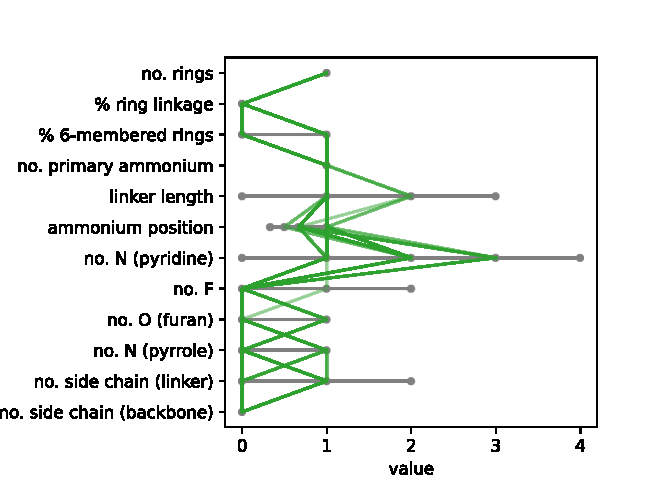
\includegraphics[width=0.8\textwidth]{figures/synthesis-feasibility/figure5-18.pdf}
    \caption{The explored fingerprint range and vs. fingerprint range of type IIb final organic spacer candidate.}
    \label{fig:figure5.18}
\end{figure}

For Type IIb spacers, the identified fingerprint set corresponds to 823 organic spacers. After applying synthesis feasibility screening, 58 candidates remained as final selections.

The fingerprint range of the final synthesizable candidates is shown in Figure \ref{fig:figure5.18}. Compared to other alignment types, the distribution suggests that Type IIb spacers exhibit less variation in backbone and tethering group features, while showing greater diversity in heteroatom substitutions and side-chain modifications. These candidates primary exhibit the following key structural characteristics:

-	Conjugated backbone: Typically one ring, either 5-membered or 6-membered.

-	Tethering ammonium group: One primary ammonium group, mostly with a single carbon in the linker.

-	Heteroatom substitutions: Presence of one or more pyridine-type nitrogen substitutions.

-	Side-chain variations: Broader diversity compared to other alignment types.

The organic spacer structures are presented in Figure \ref{fig:figure5.19}. Interestingly, we observed that multiple Type IIb organic spacers often share identical fingerprints.

\begin{figure}[htbp]
    \centering
    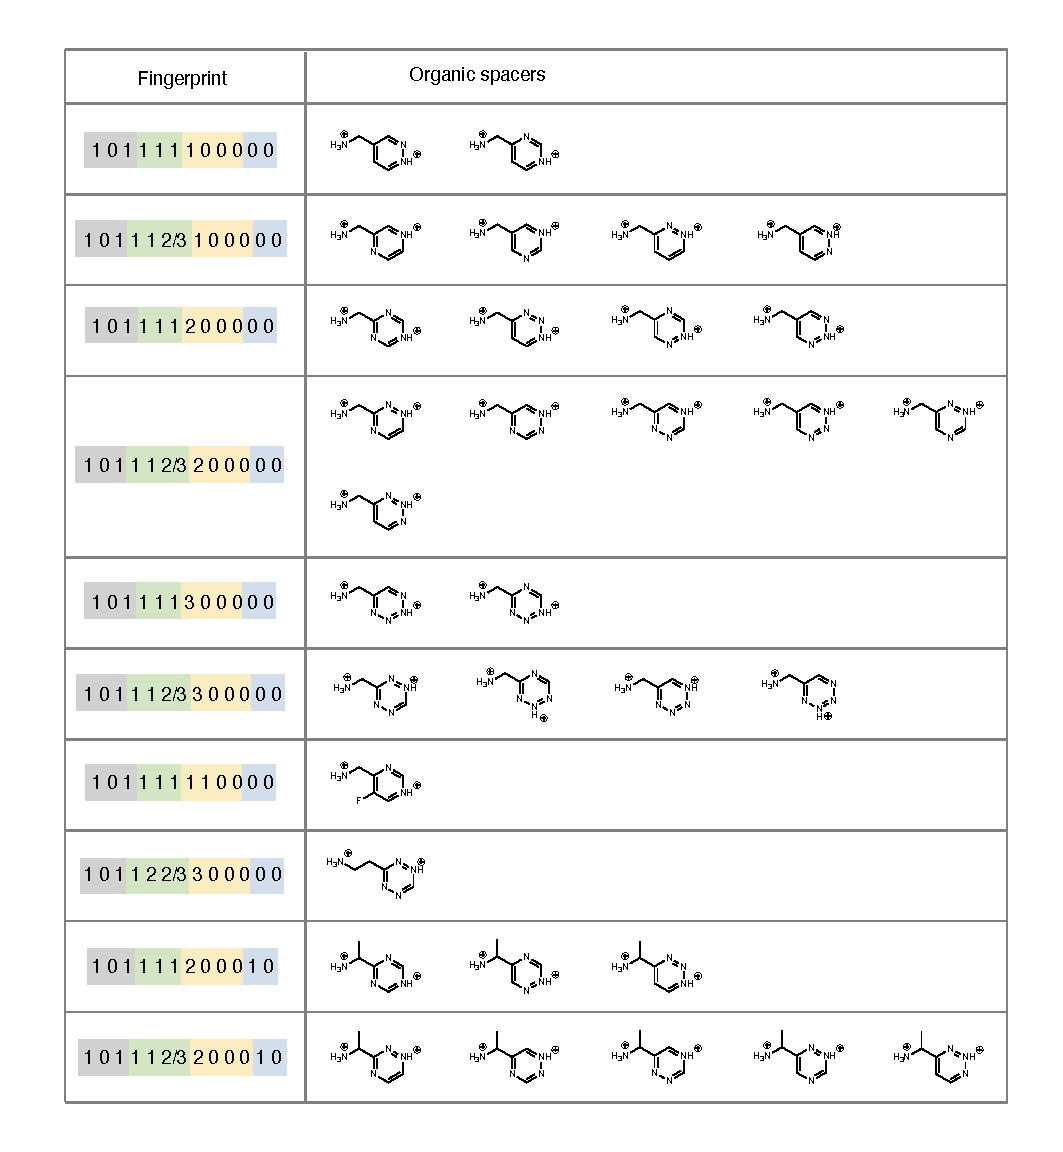
\includegraphics[width=\textwidth]{figures/synthesis-feasibility/figure5-19-1.pdf}
    \caption{Inverse designed candidates for type IIb alignment (Part 1).}
    \label{fig:figure5.19}
\end{figure}

\begin{figure}[htbp]
    \ContinuedFloat
    \centering
    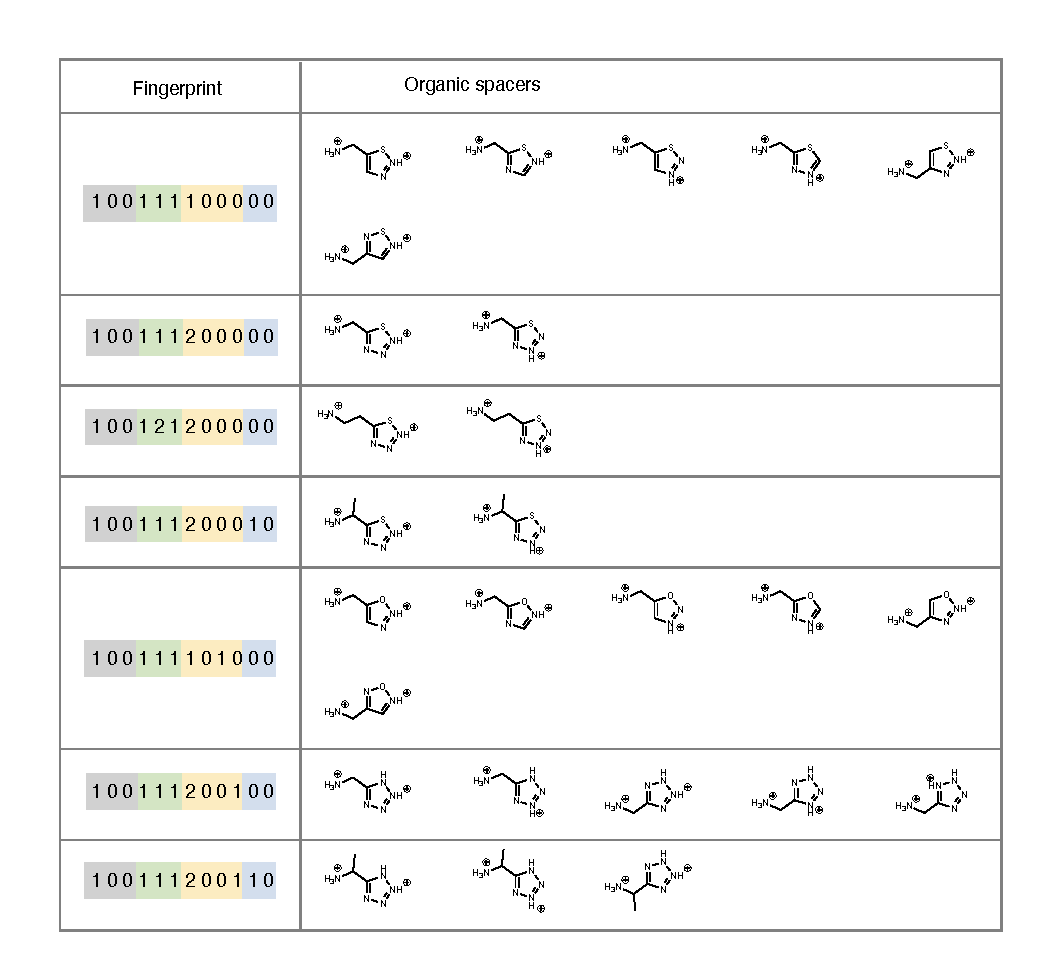
\includegraphics[width=\textwidth]{figures/synthesis-feasibility/figure5-19-2.pdf}
    \caption{Inverse designed candidates for type IIb alignment (Part 2, continued).}
\end{figure}

\subsection{DFT validation of designed DJ perovskites}

\begin{figure}[htbp]
    \centering
    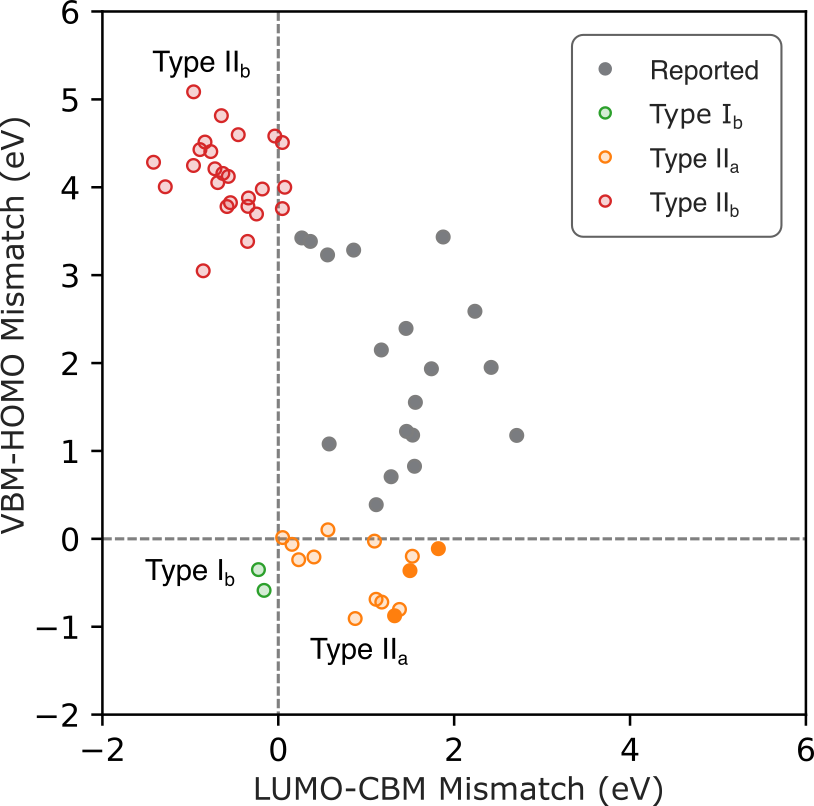
\includegraphics[width=0.6\textwidth]{figures/synthesis-feasibility/figure5-20.png}
    \caption{Scatter plot depicting the predicted DJ perovskites with targeted alignment types (Ib, IIa, and IIb) alongside previously reported structures.}
    \label{fig:figure5.20}
\end{figure}

We constructed DJ perovskite structures based on the designed organic spacers and performed DFT calculations to validate their energy level alignments. The DFT validation results, summarized in Figure \ref{fig:figure5.20}, compare all final candidates with experimentally reported DJ perovskites. The newly identified organic spacers significantly expand the energy level alignment landscape, covering a much broader range than previously reported structures. Notably, most of the inverse-designed structures exhibit the targeted energy level alignment, demonstrating the effectiveness of our AI-assisted inverse design workflow.

In the following sections, we discuss the discovered organic spacers for each energy level alignment type, along with key molecular design insights. We show that all selected organic spacers originate from well-established research fields:
\begin{itemize}
    \item Type Ib and Type IIa candidates are primarily derived from organic electronics and optoelectronic research \cite{RN628, RN632}, including acene- and oligothiophene-based molecules.
    \item Type IIb candidates are predominantly associated with medicinal chemistry, featuring structures such as diazine-based molecules.
\end{itemize}


\textbf{Type Ib energy level alignment}

Designing type Ib spacers proved the most challenging due to the need for a highly conjugated backbone with small HOMO-LUMO gap. Our analysis revealed that only acene-based spacers with at least five linearly fused benzene rings can achieve the required small HOMO-LUMO gap (< 2.3 eV, below the inorganic bandgap). Other conjugated backbones, such as benzene (linked) or thiophene (either linked or fusion) with a comparable number of rings, are ineffective. 

Acene-based materials, extensively studied in organic electronics\cite{RN632}, exhibit a progressively narrowing HOMO-LUMO gap as the number of rings increases. 

Both two identified type Ib spacers feature a pentacene backbone with two ammonium tethering groups. While higher acene derivatives (e.g., hexacene, heptacene) could theoretically achieve even smaller HOMO-LUMO gaps and guarantee type Ib alignment, they were absent from the PubChem database, likely due to the limited chemical stability of higher acenes. 

\begin{figure}[htbp]
    \centering
    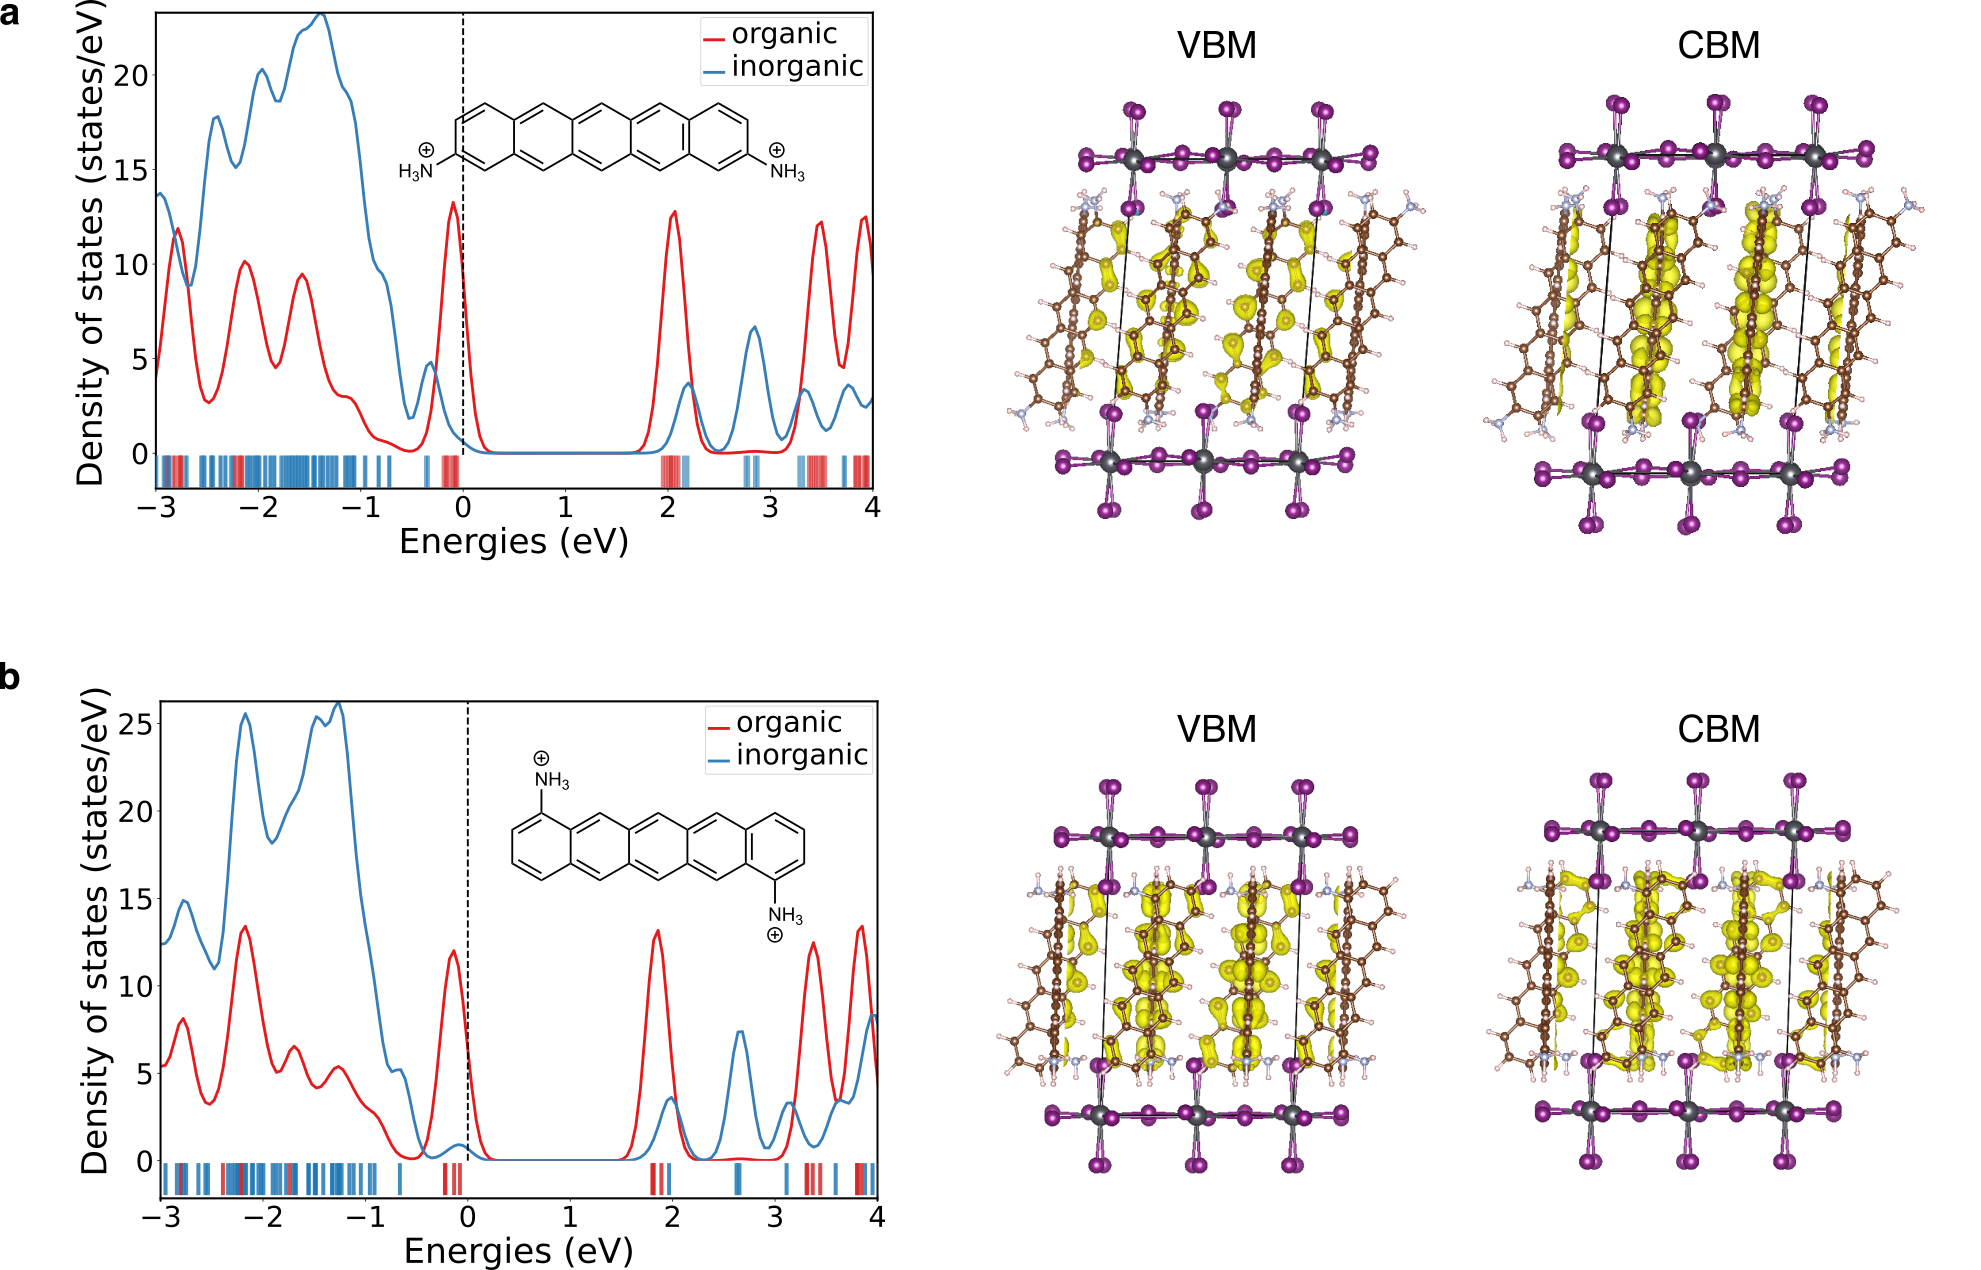
\includegraphics[width=\textwidth]{figures/synthesis-feasibility/figure5-21.png}
    \caption{Electronic structure of final candidate selections for type Ib DJ perovskites.}
    \label{fig:figure5.21}
\end{figure}


 The electronic structure of the two proposed DJ perovskites exhibiting Type Ib alignment is shown in Figure \ref{fig:figure5.21}. The left panels display the projected density of states (PDOS), illustrating the electronic contributions from the organic (red) and inorganic (blue) components, with the Fermi level set to 0 eV (dashed line). The right panels show the charge density distributions of the band edge states (VBM and CBM). The yellow isosurfaces indicate the spatial distribution of electronic states, confirming that both the VBM and CBM of the DJ perovskite are primarily contributed by the organic component. Moreover, the HOMO and LUMO of the organic spacers are predominantly localized along the pentacene backbone, where the $\pi$-electron density is most concentrated and delocalized.

\textbf{Comparison with reported 2D perovskites}

To date, only one diammonium organic spacer featuring type Ib alignment has been theoretically designed in DJ lead-iodide perovskites\cite{RN2}. This spacer, which also features a pentacene backbone with two methylammonium tethering groups, was identified in our inverse design (appear in $G_4$), but was excluded in the subsequent PubChem filtering step. 

The only experimentally synthesized 2D lead-iodide perovskite spacer with type Ib alignment belong to RP phase\cite{RN20}.In that study, Type Ib alignment was inferred based on photoluminescence (PL) emission from the organic component and qualitative energy level estimations using a series of approximations. However, relying on optical properties alone to deduce electronic alignment is questionable, as optical gaps do not always directly correspond to electronic energy levels. Moreover, their DFT calculations suggested a mixed alignment between Type IIa and Type Ib, with a mixing factor of 0.25. 

Our calculations (Figure \ref{fig:figure5.22}), performed using the same perovskite structure as in their study, indicate that the alignment is actually Type IIa, regardless of whether we apply the systematic mixing factor of 0.4 used throughout our study or the 0.25 mixing factor employed in the previous work. The discrepancy in computational results is likely due to differences in software implementations and methodological choices.

While direct comparisons across different simulation methodologies and experimental techniques remain challenging in 2D perovskite research\cite{RN38}, the relative trends within our calculations—conducted with a consistent set of computational parameters—are internally reliable. These findings suggest that our proposed pentacene-based organic spacers provide a more precise and controllable approach for achieving Type Ib energy level alignment in 2D perovskites.

\begin{figure}[htbp]
    \centering
    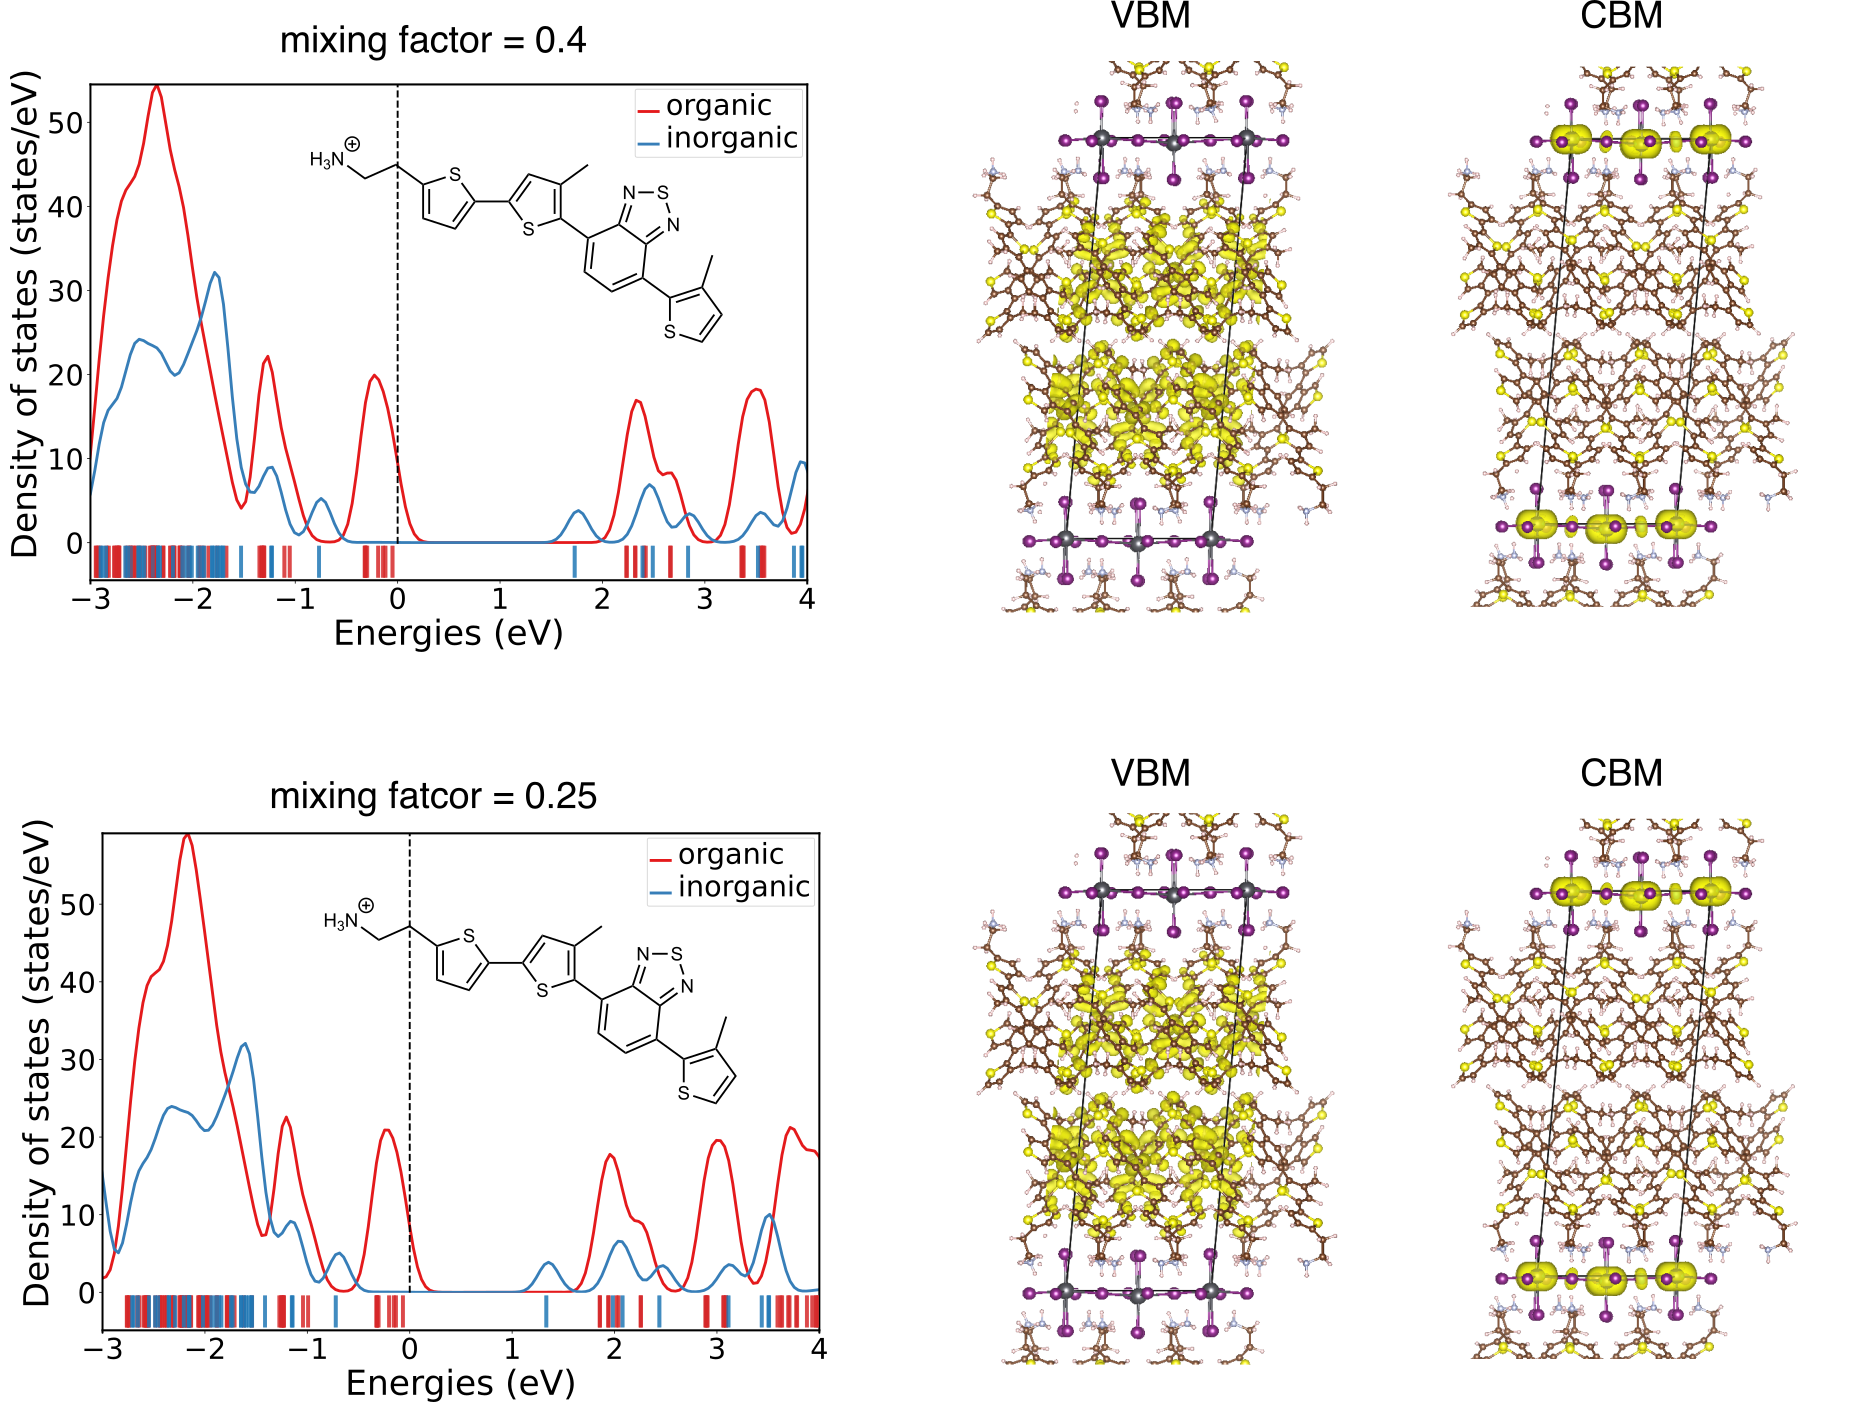
\includegraphics[width=\textwidth]{figures/synthesis-feasibility/figure5-22.png}
    \caption{Energy level alignment of the previously reported RP-phase spacer claimed to exhibit type Ib alignment. }
    \label{fig:figure5.22}
\end{figure}

\textbf{Type IIa energy level alignment}

Achieving Type IIa alignment typically requires extended conjugation through an increased number of aromatic rings to raise the HOMO energy level. Our inverse design approach identified two major families of organic spacers that satisfy these criteria: acene-based molecules with fewer rings than pentacene and oligothiophene-based molecules. It is well established in organic chemistry that both families exhibit a progressively narrower HOMO-LUMO gap as the ring count increases.

In the context of organic spacers, these molecules rely on the same principle—extending conjugation to elevate HOMO energy levels and reduce LUMO levels. Additionally, our analysis indicates that increasing the linker length in the tethering ammonium group raises both HOMO and LUMO energy levels, further influencing energy alignment.

The electronic structures of the 12 DJ perovskites structures exhibiting type IIa alignment are shown in Figure \ref{fig:figure5.23}. The VBM is primarily contributed by the organic component, while the CBM remains dominated by the inorganic framework.

Within the oligothiophene family, all identified organic spacers feature linked thiophene rings with variable ring counts and different linker lengths. This family represents one of the earliest explored organic spacers in 2D perovskites, and three of these spacers (Figure \ref{fig:figure5.23}a,c,e) have already been reported in the literature \cite{RN18, RN38}.


\begin{figure}[htbp]
    \centering
    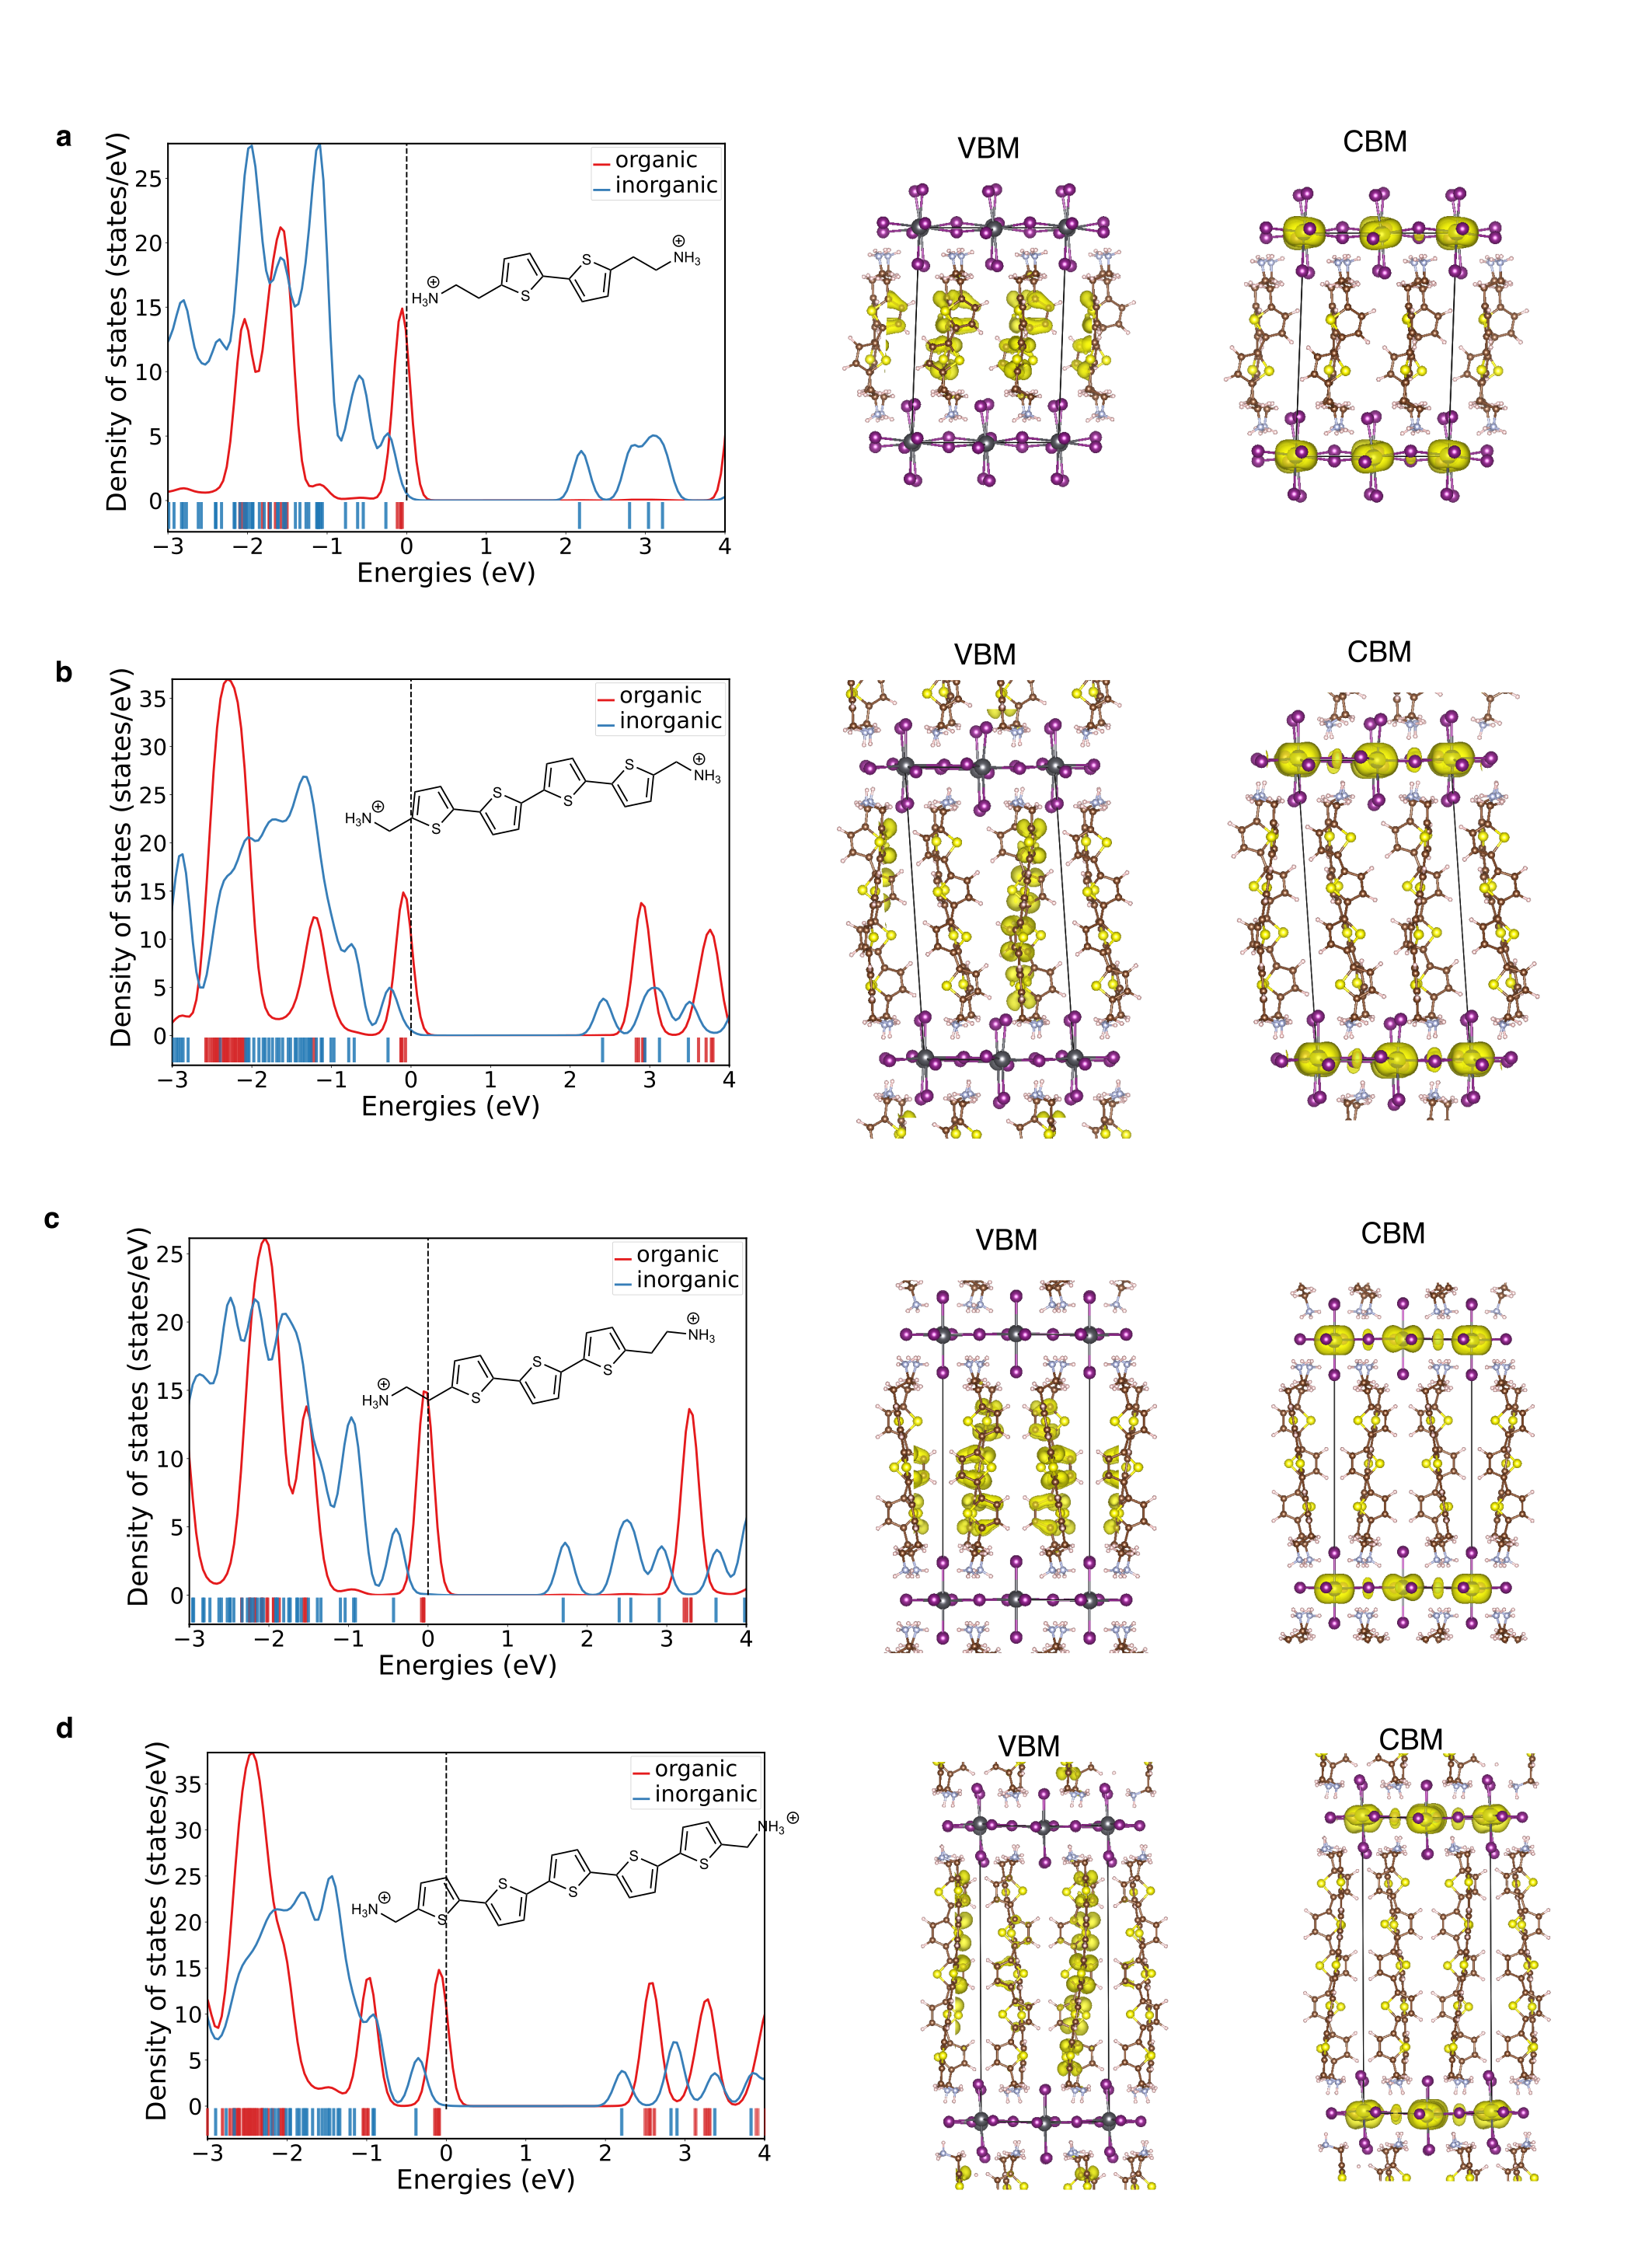
\includegraphics[width=0.9\textwidth]{figures/synthesis-feasibility/figure5-23-1.png}
    \caption{Electronic structure of inverse-designed type IIa DJ perovskites (Part 1).}
    \label{fig:figure5.23}
\end{figure}

\begin{figure}[htbp]
    \ContinuedFloat
    \centering
    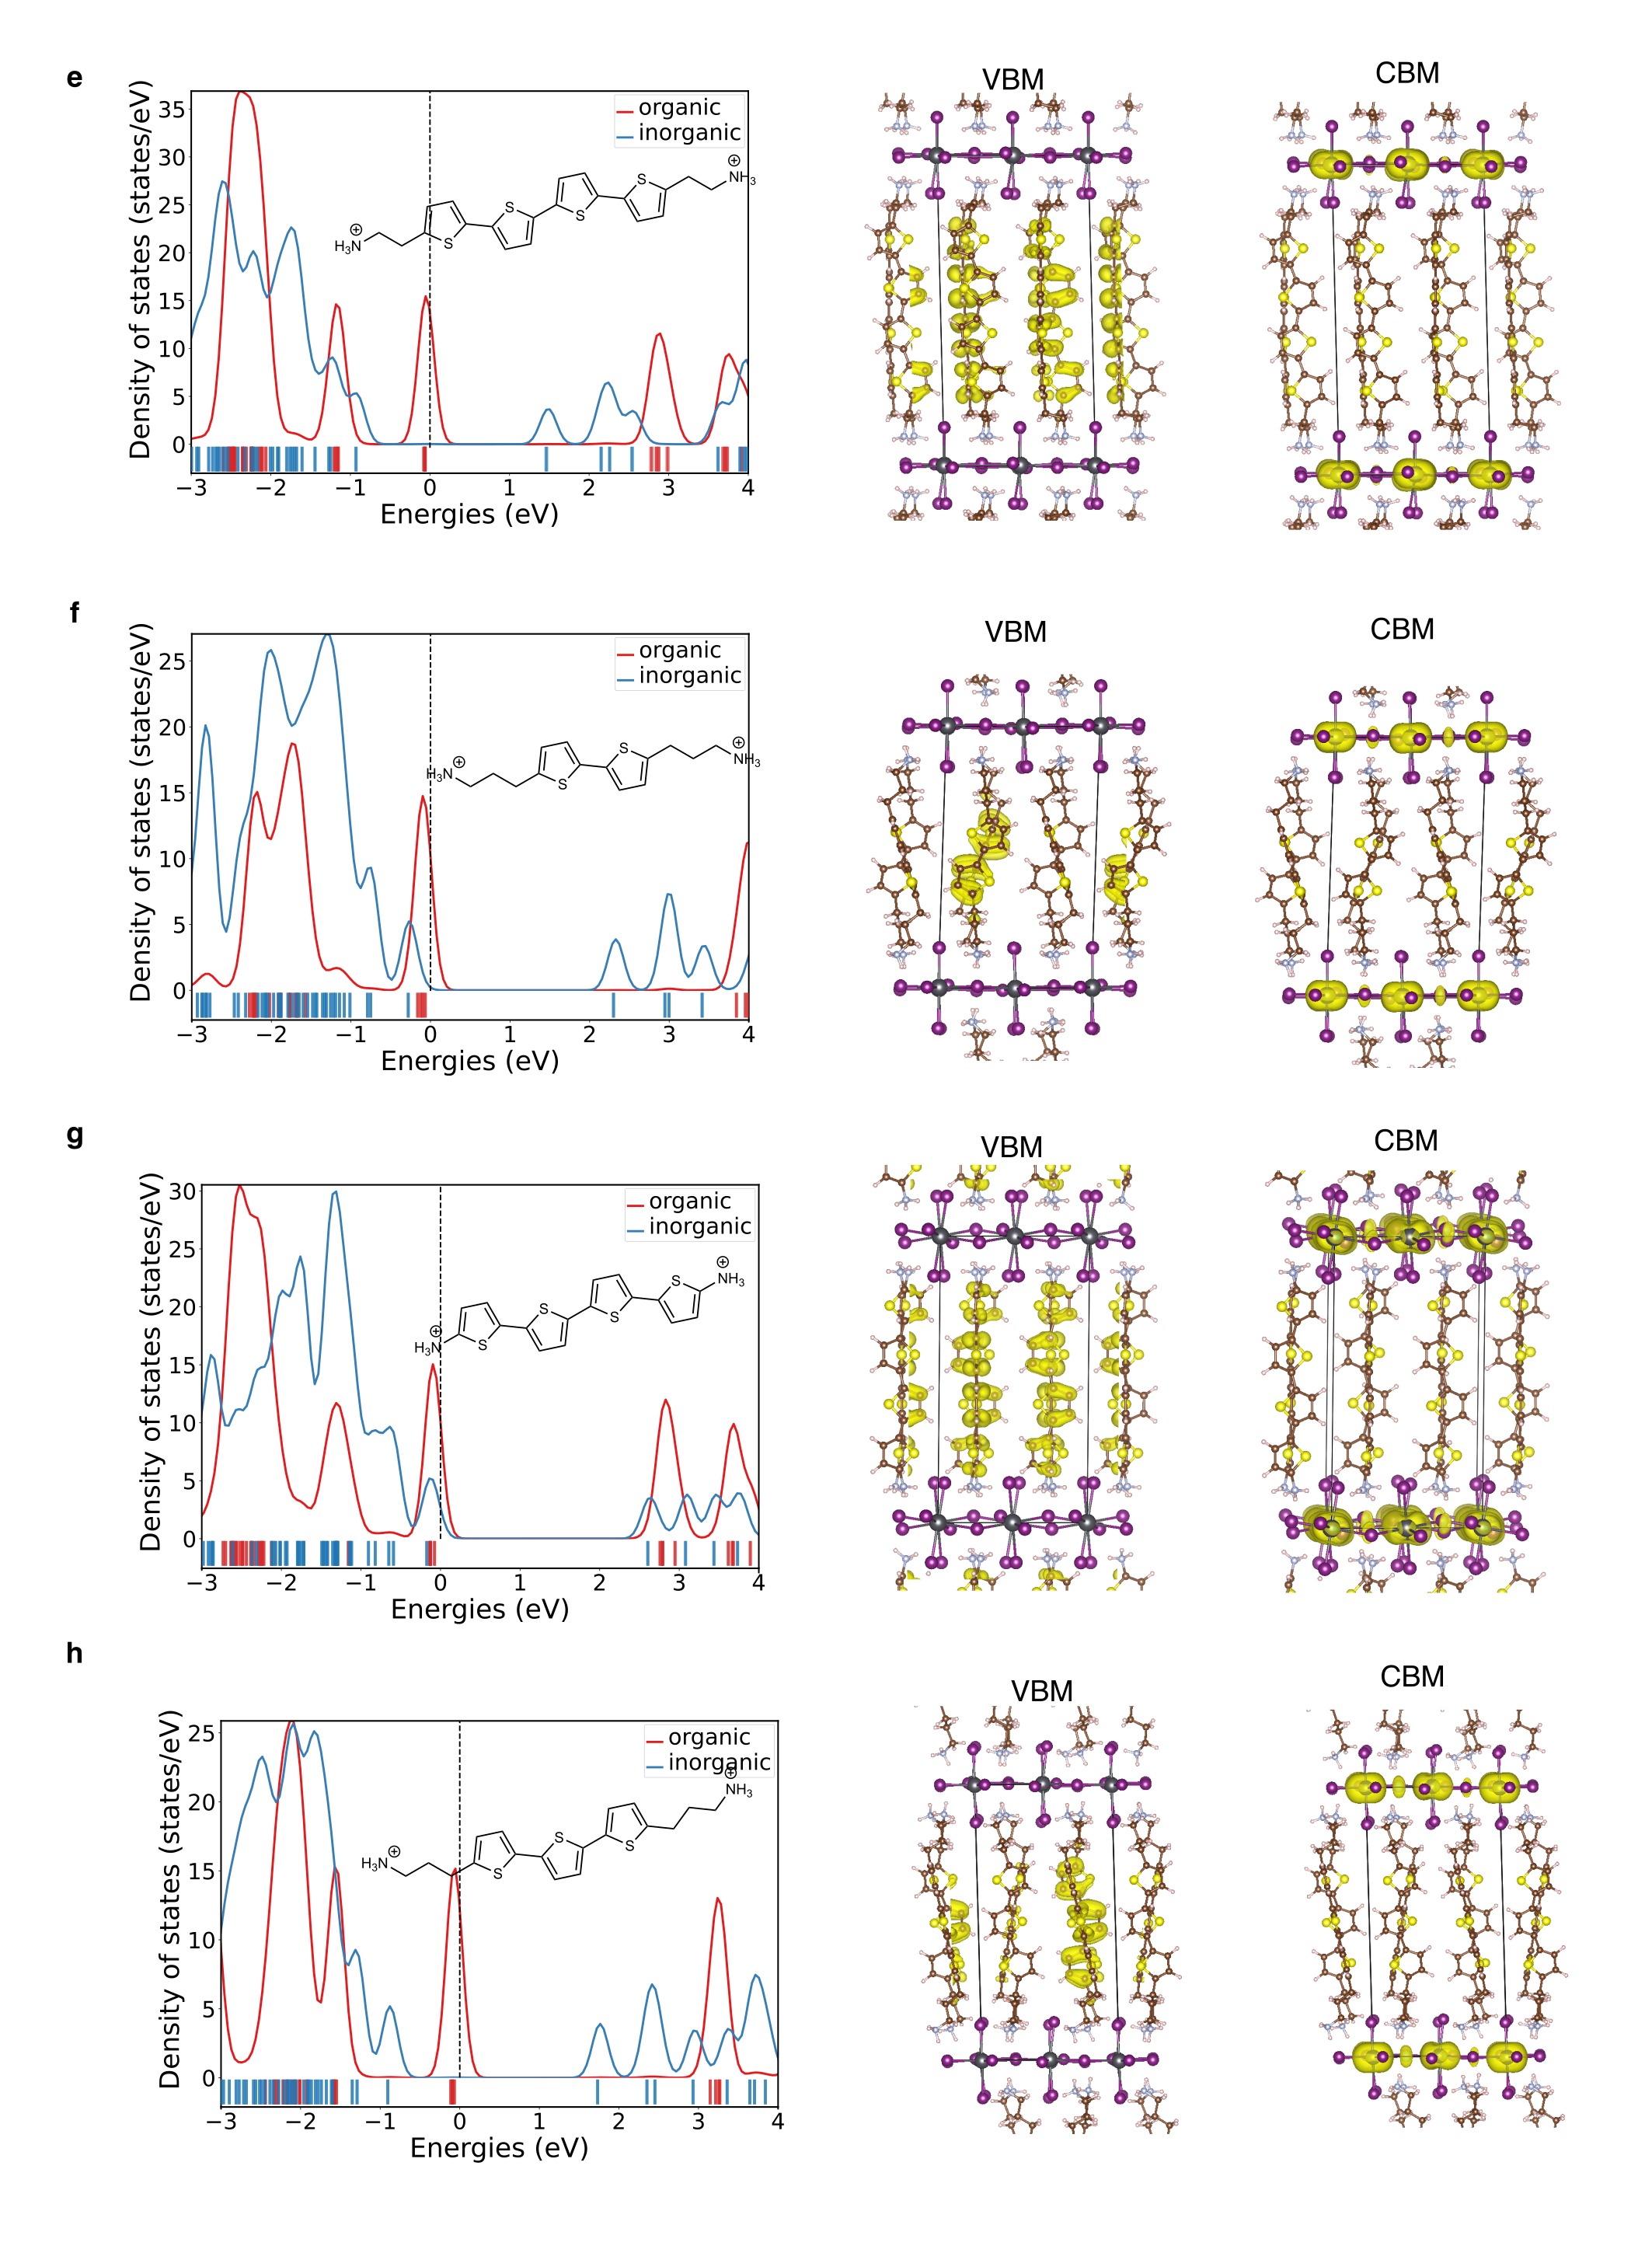
\includegraphics[width=0.9\textwidth]{figures/synthesis-feasibility/figure5-23-2.png}
    \caption{Electronic structure of inverse-designed type IIa DJ perovskites (Part 2, continued).}
\end{figure}

\begin{figure}[htbp]
    \ContinuedFloat
    \centering
    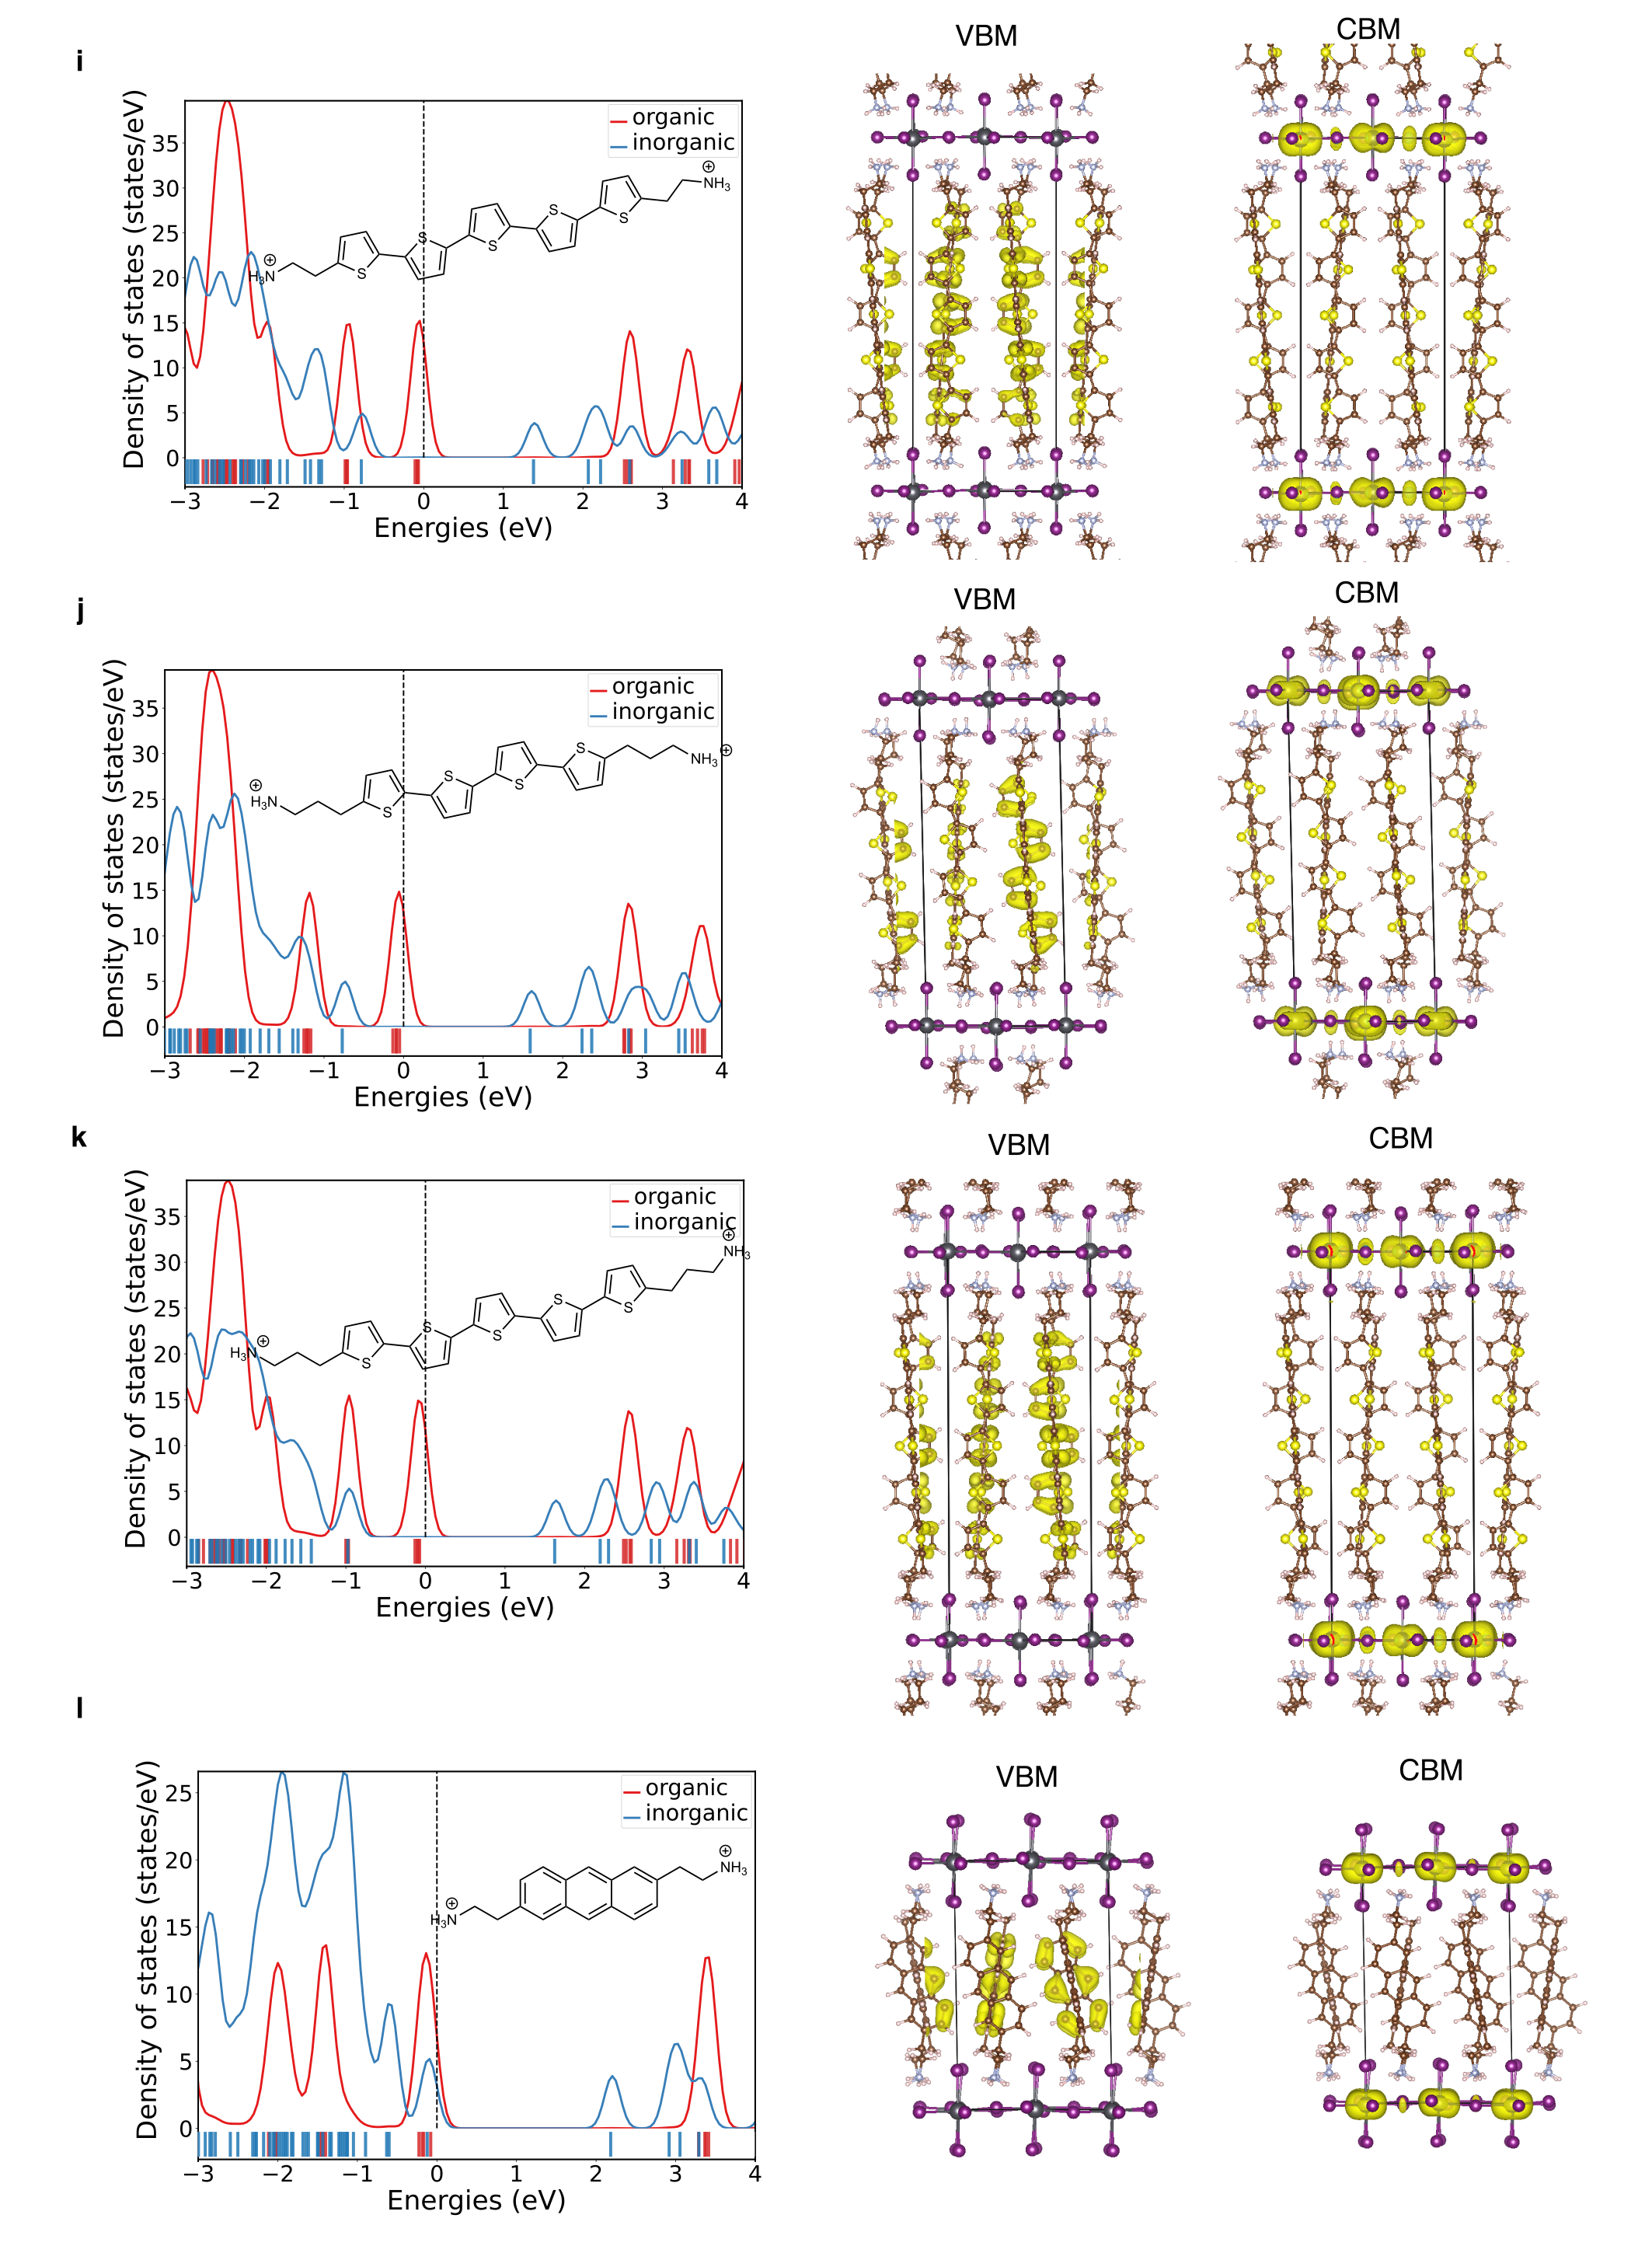
\includegraphics[width=0.9\textwidth]{figures/synthesis-feasibility/figure5-23-3.png}
    \caption{Electronic structure of inverse-designed type IIa DJ perovskites (Part 3, continued).}
\end{figure}

Only one acene-based spacer (Figure \ref{fig:figure5.23}l) was confirmed to exhibit Type IIa alignment, featuring anthracene with an ethylammonium tethering group. This molecule has been extensively studied in a theoretical work \cite{RN2}, where it was reported to exhibit a mixed Type IIa/Ia alignment. The slight mismatch with our findings is likely due to differences in structural details; however, the overall trend remains consistent between our study and previous research.


\textbf{Type IIb energy level alignment}

Type IIb spacers typically require a single primary ammonium group and pyridine-type nitrogen substitutions at multiple positions on aromatic rings to effectively lower the LUMO level. These organic spacers frequently feature nitrogen-substituted ring systems as their conjugated backbone, which are well-established in medicinal chemistry and related fields. For example, our study identified several organic spacers containing six-membered aromatic diazines, including pyrazine, pyridazine, and pyrimidine. Two of these spacers were previously predicted in theoretical studies with similar results \cite{RN617}; however, to date, no experimental studies have been conducted on DJ perovskites featuring Type IIb alignment.

Compared to the only known spacer reported in the RP phase, our identified spacers exhibit significantly simpler structures, suggesting improved synthetic accessibility and potential for experimental realization.

The electronic structure of the Type IIb DJ perovskites is shown in Figure \ref{fig:figure5.25}. The bottom panel of the partial density of states (PDOS) displays the energy levels at the Z-point and $\Gamma$-point, respectively. Differences in energy levels between these two points indicate the presence of interlayer coupling between inorganic layers. Notably, most structures exhibit significant interlayer coupling, due to the small size of organic spacers within this alignment type.

\begin{figure}[htbp]
    \centering
    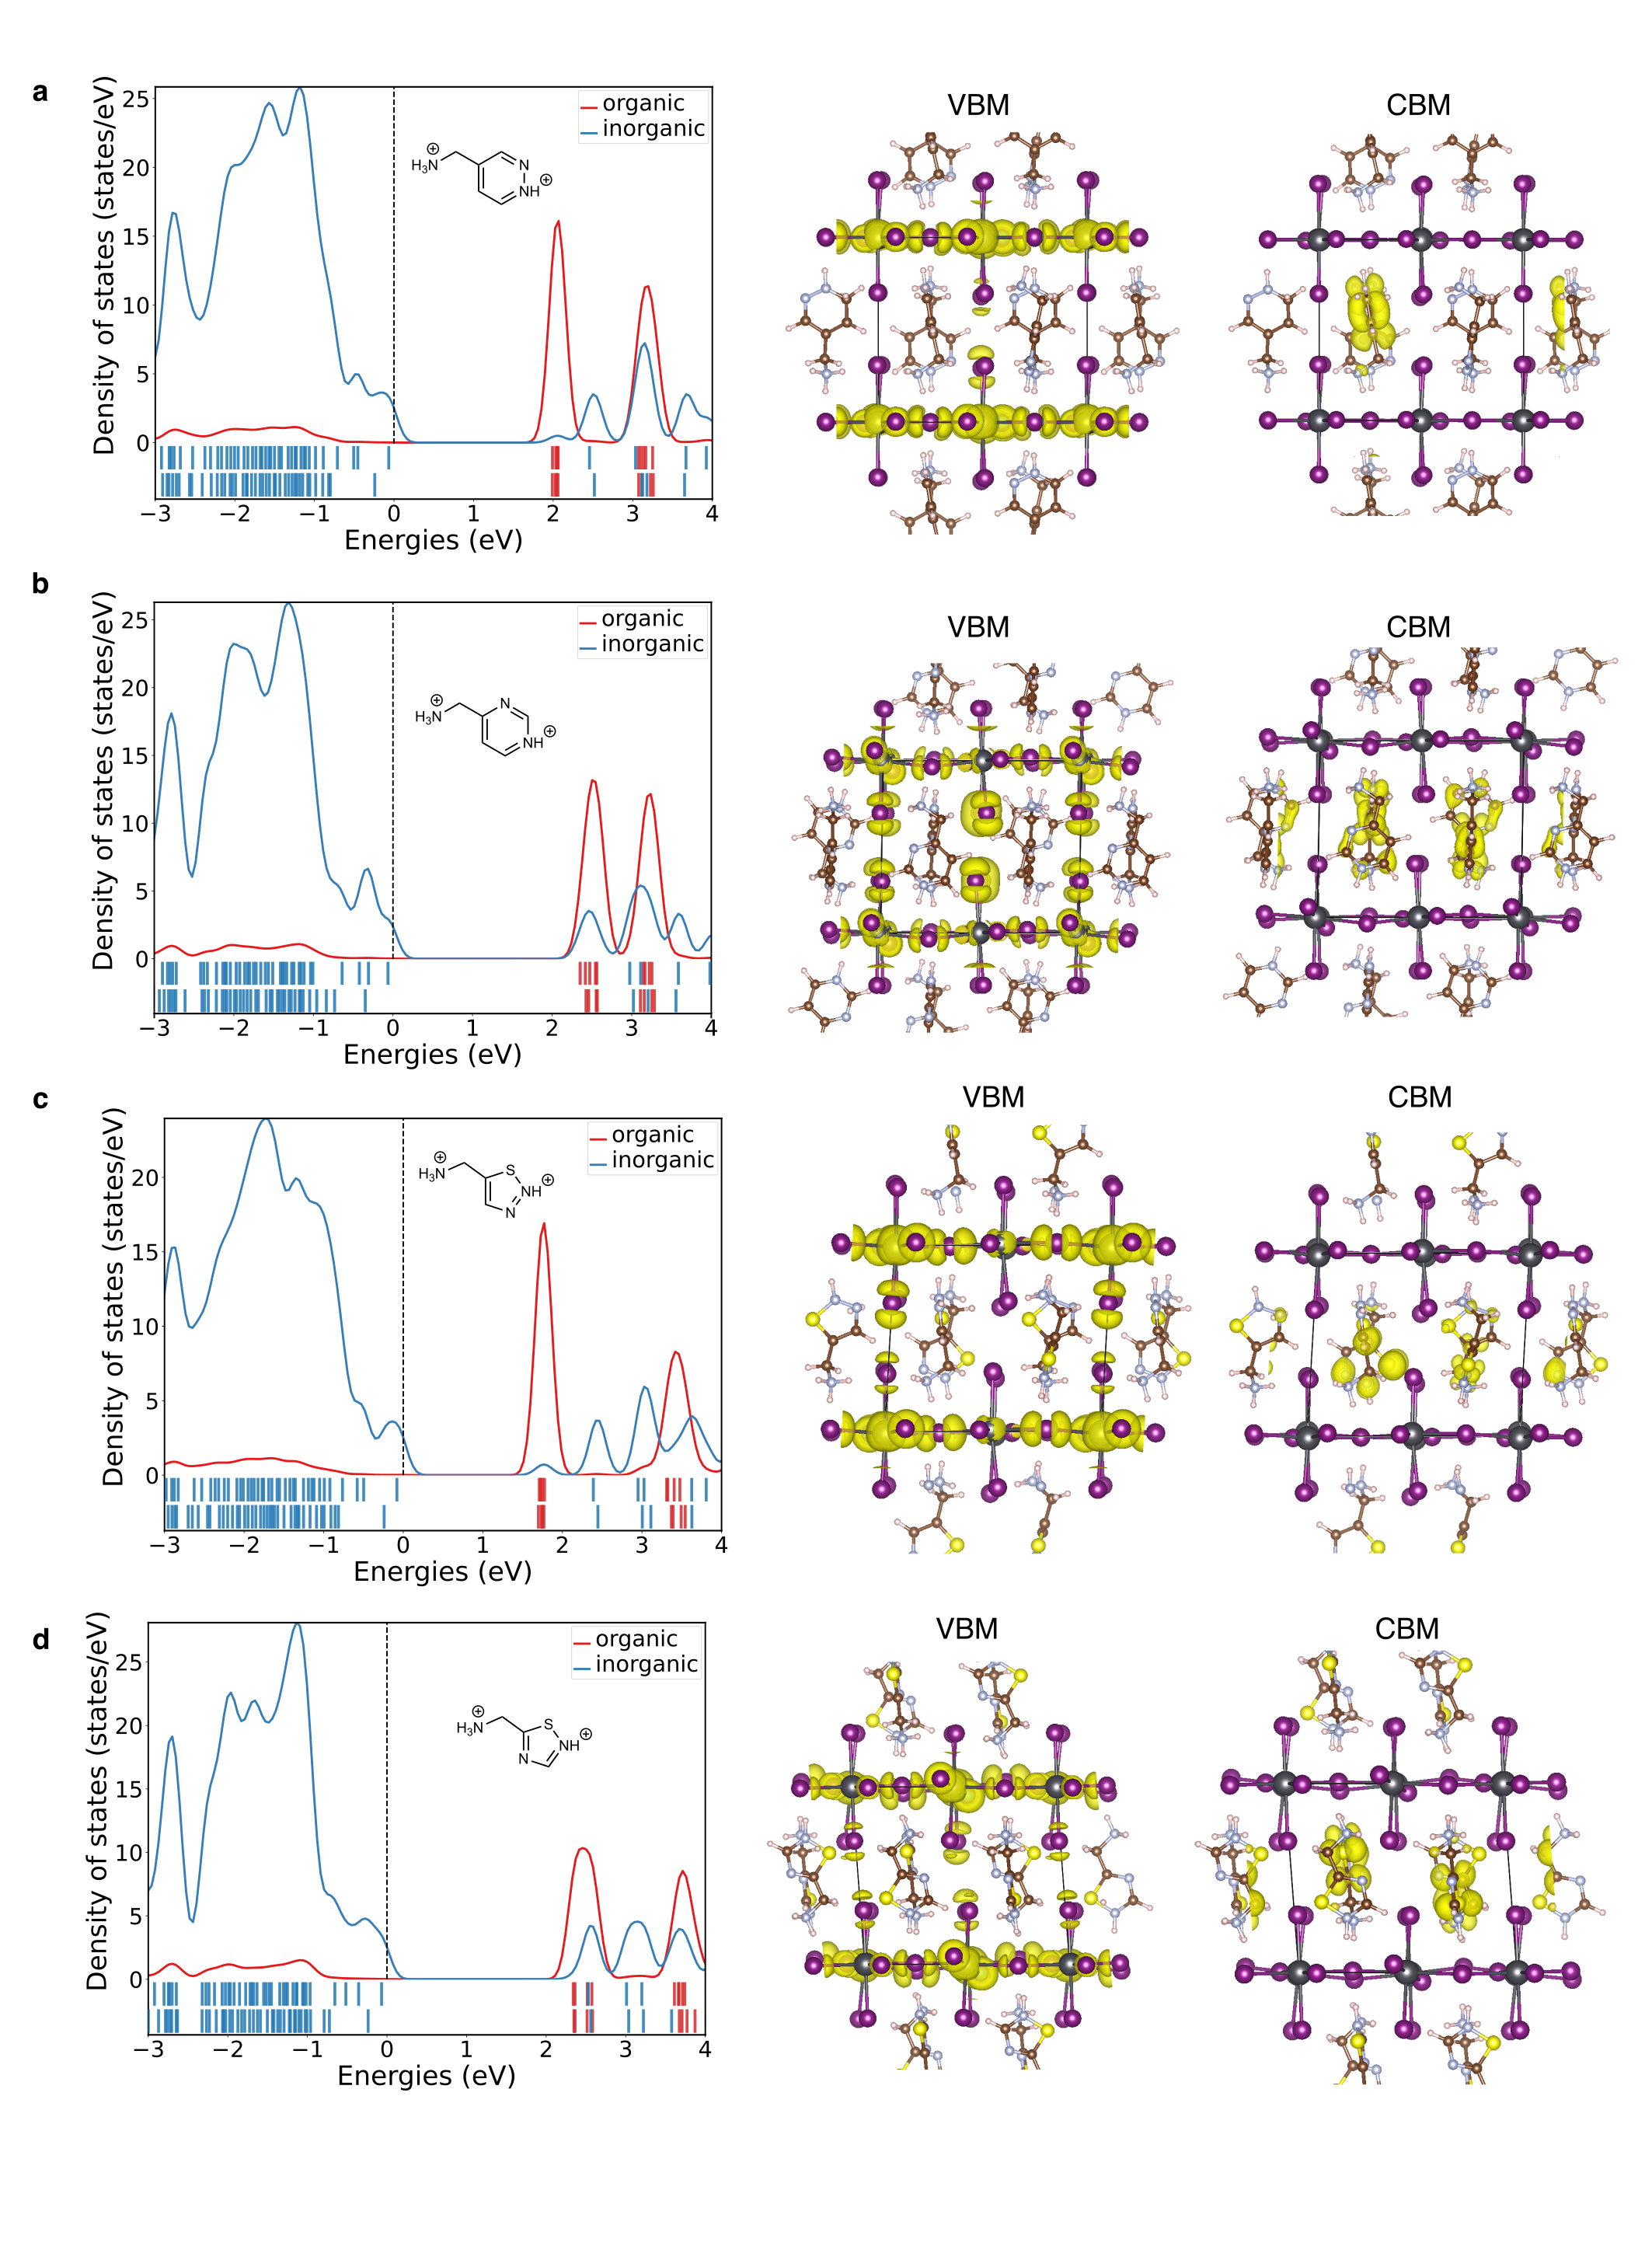
\includegraphics[width=0.9\textwidth]{figures/synthesis-feasibility/figure5-25-1.png}
    \caption{Electronic structure of inverse-designed type IIb DJ perovskites (Part 1).}
    \label{fig:figure5.25}
\end{figure}

\begin{figure}[htbp]
    \ContinuedFloat
    \centering
    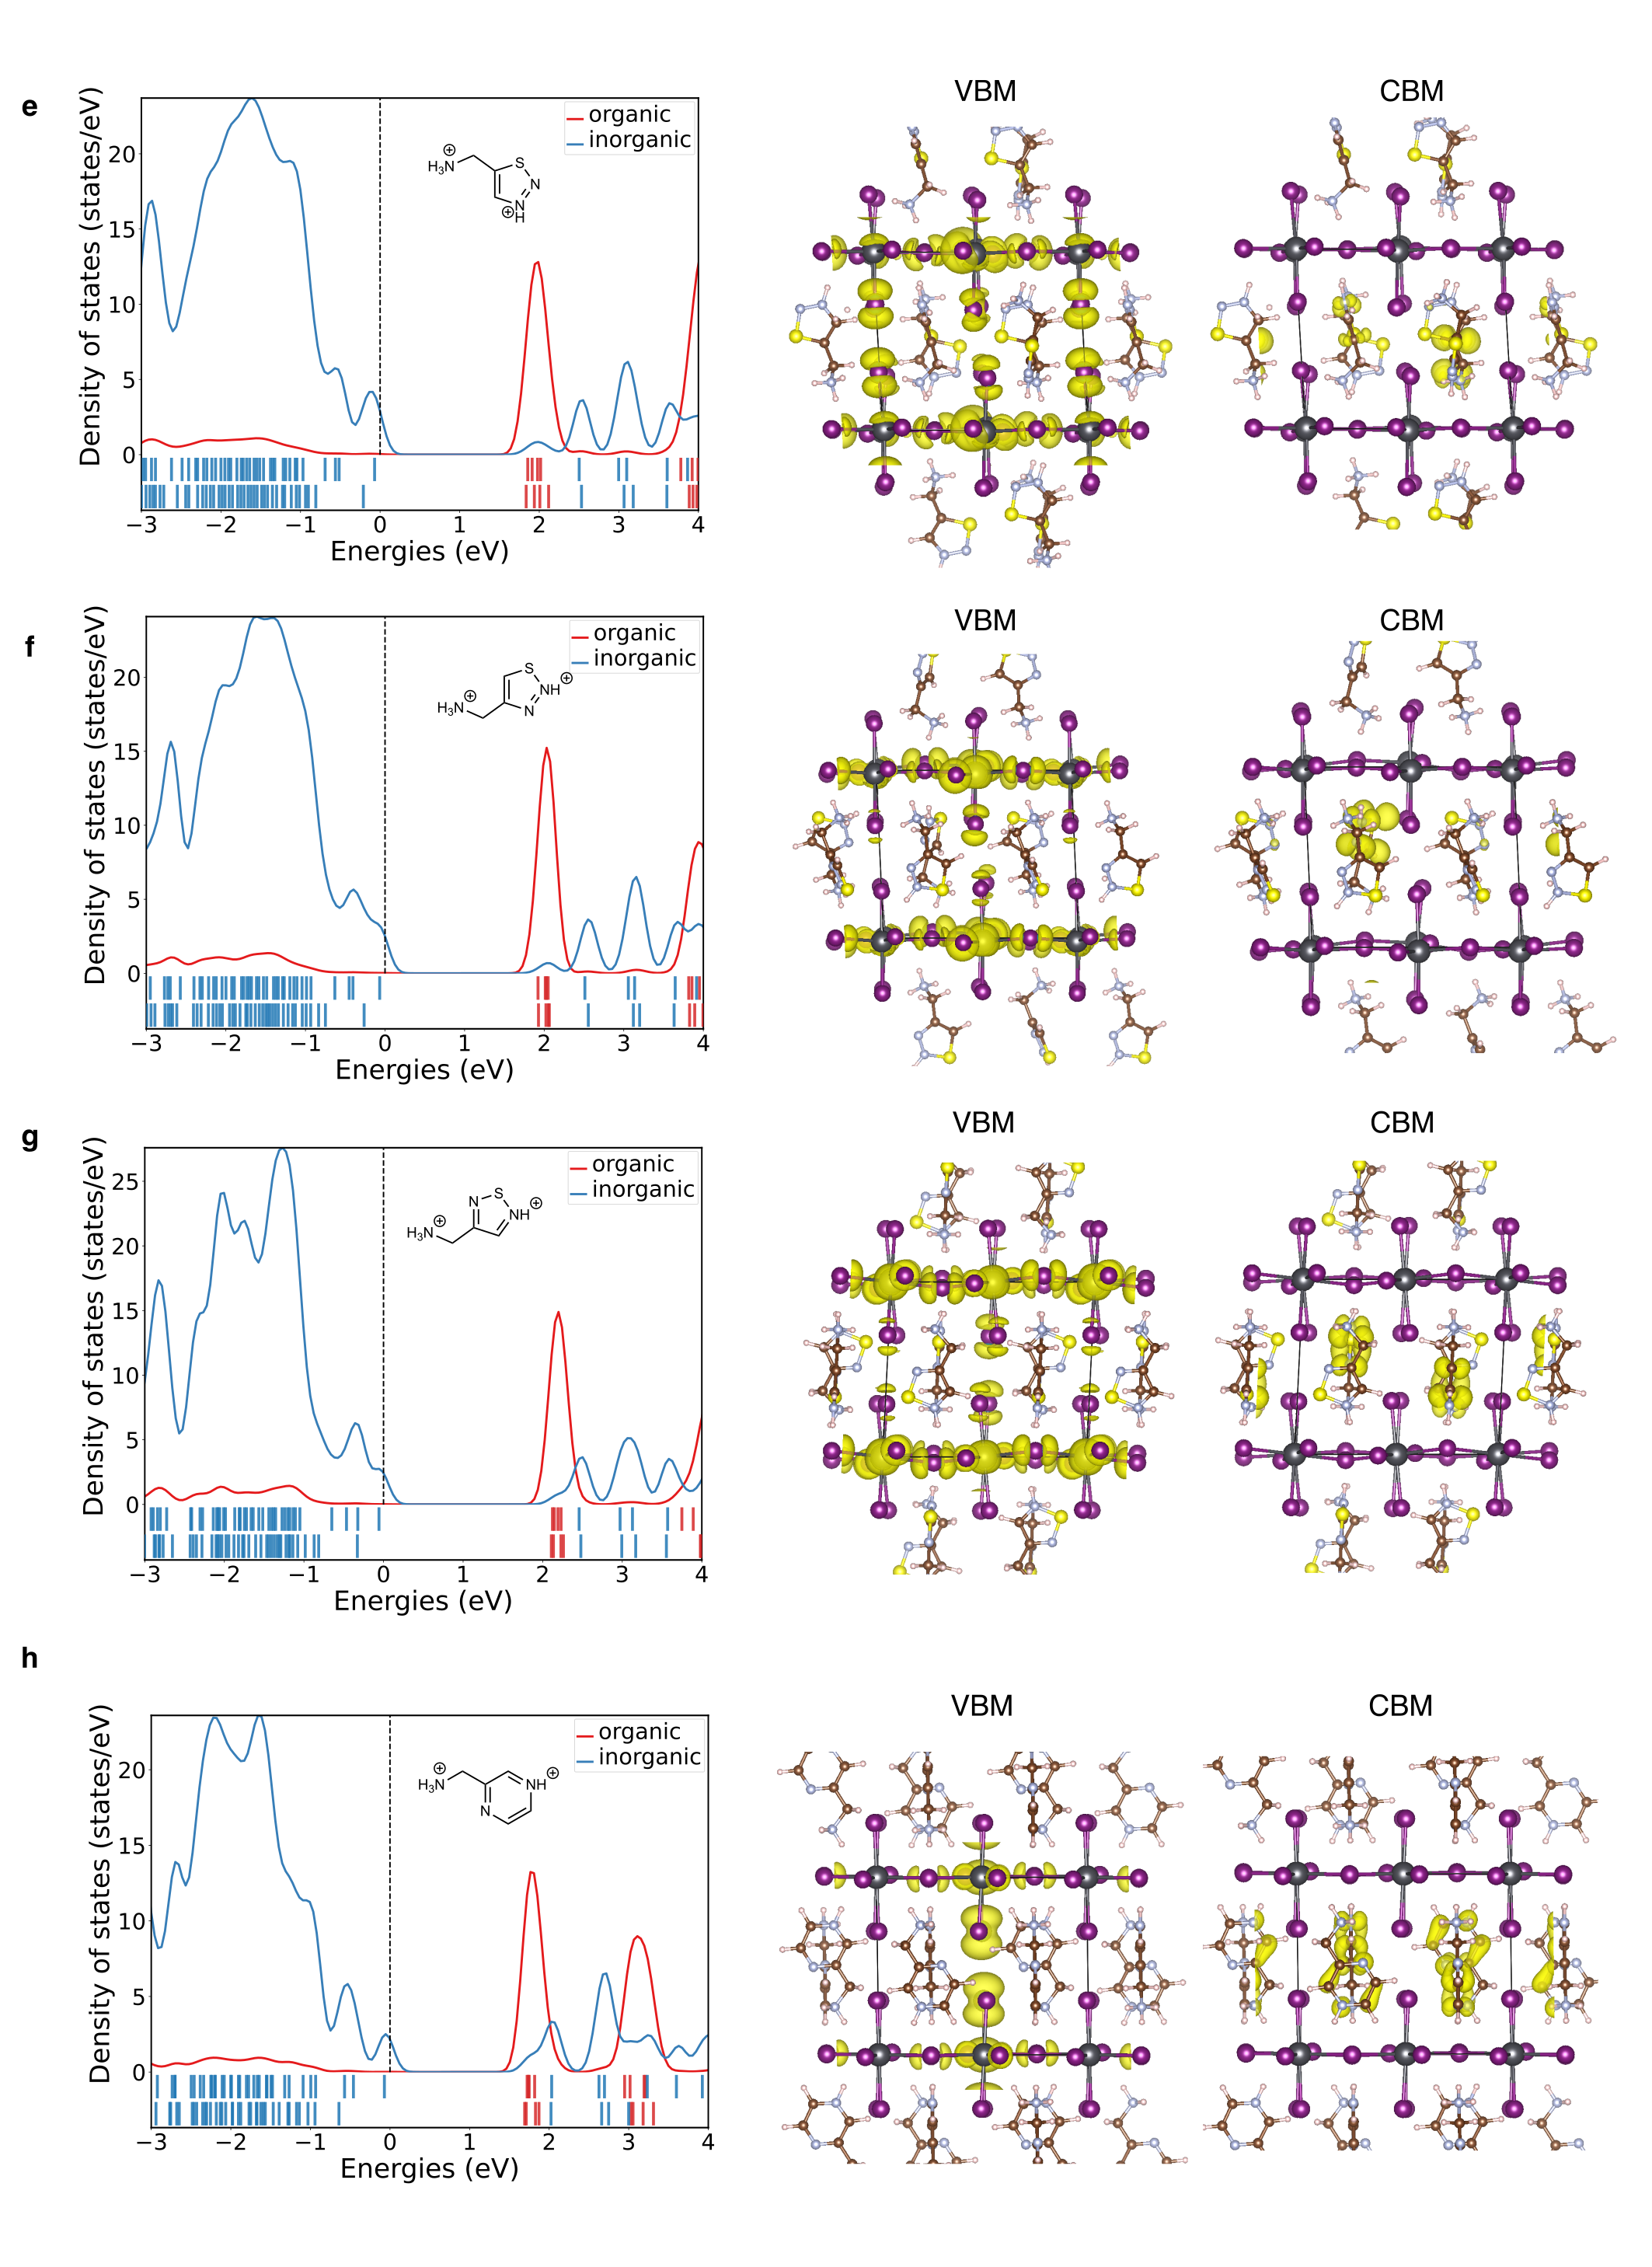
\includegraphics[width=0.9\textwidth]{figures/synthesis-feasibility/figure5-25-2.png}
    \caption{Electronic structure of inverse-designed type IIb DJ perovskites (Part 2, continued).}
\end{figure}

\begin{figure}[htbp]
    \ContinuedFloat
    \centering
    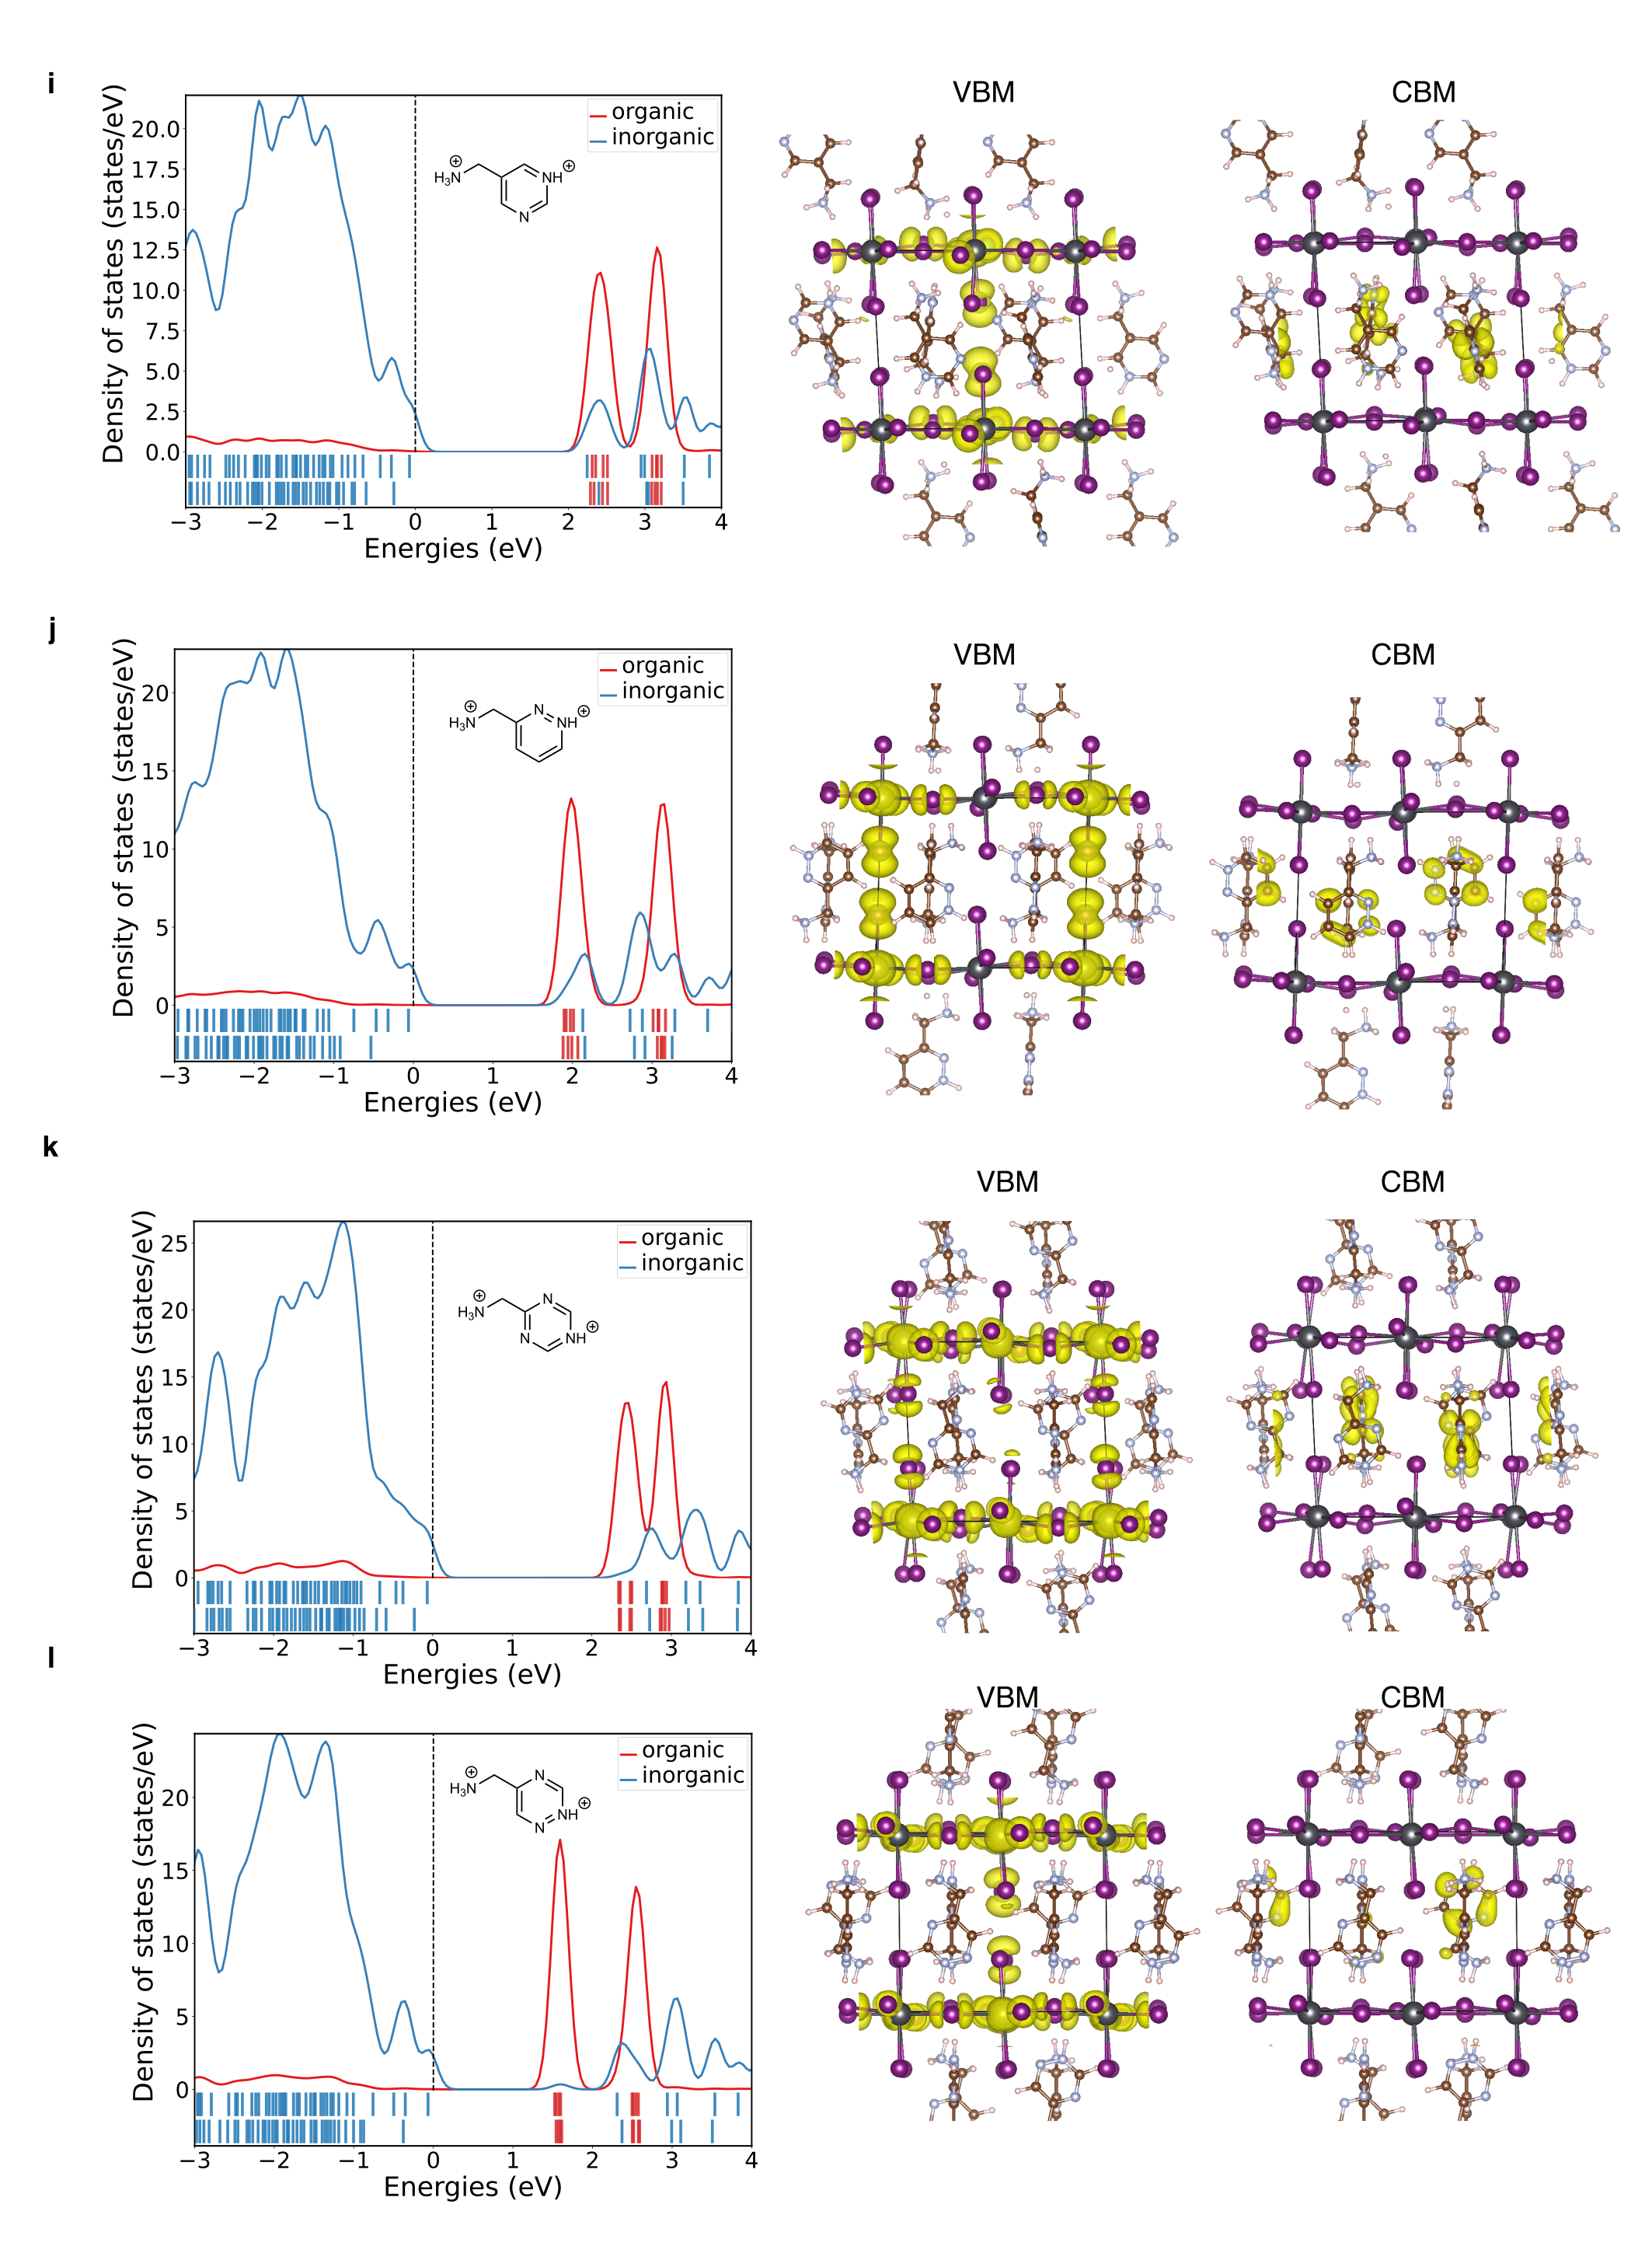
\includegraphics[width=0.9\textwidth]{figures/synthesis-feasibility/figure5-25-3.png}
    \caption{Electronic structure of inverse-designed type IIb DJ perovskites (Part 3, continued).}
\end{figure}

\begin{figure}[htbp]
    \ContinuedFloat
    \centering
    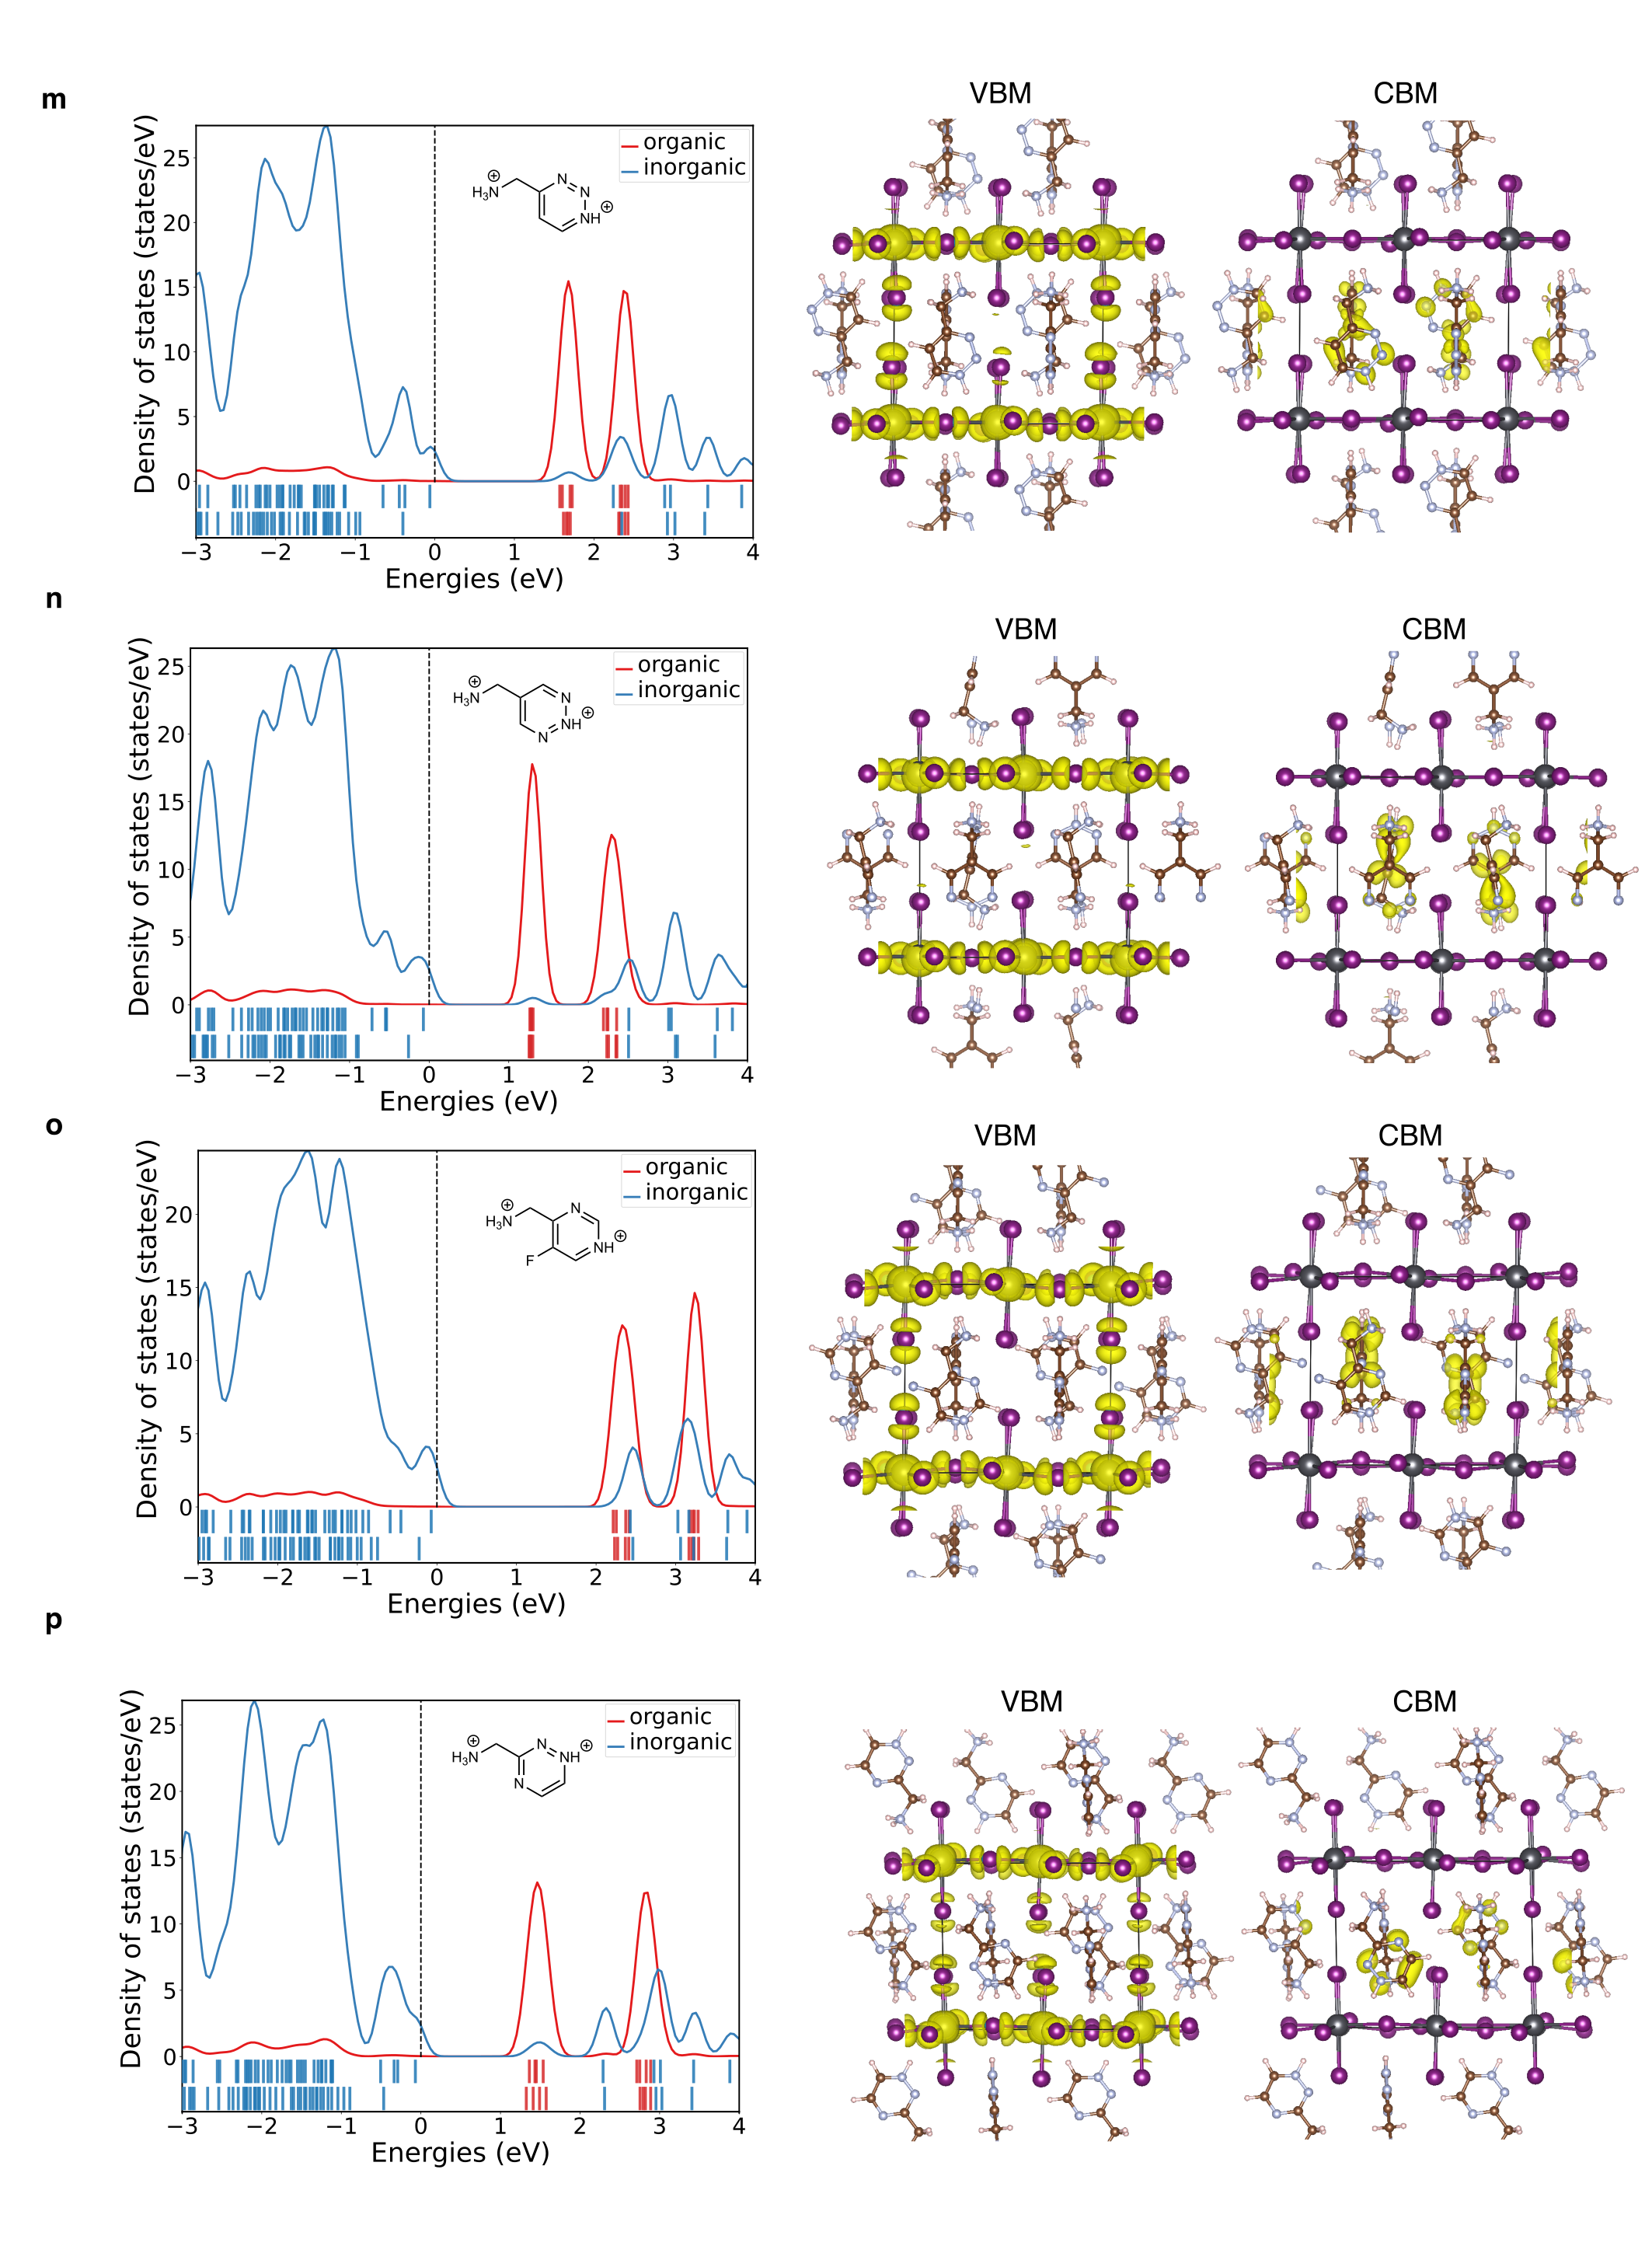
\includegraphics[width=0.9\textwidth]{figures/synthesis-feasibility/figure5-25-4.png}
    \caption{Electronic structure of inverse-designed type IIb DJ perovskites (Part 4, continued).}
\end{figure}

\begin{figure}[htbp]
    \ContinuedFloat
    \centering
    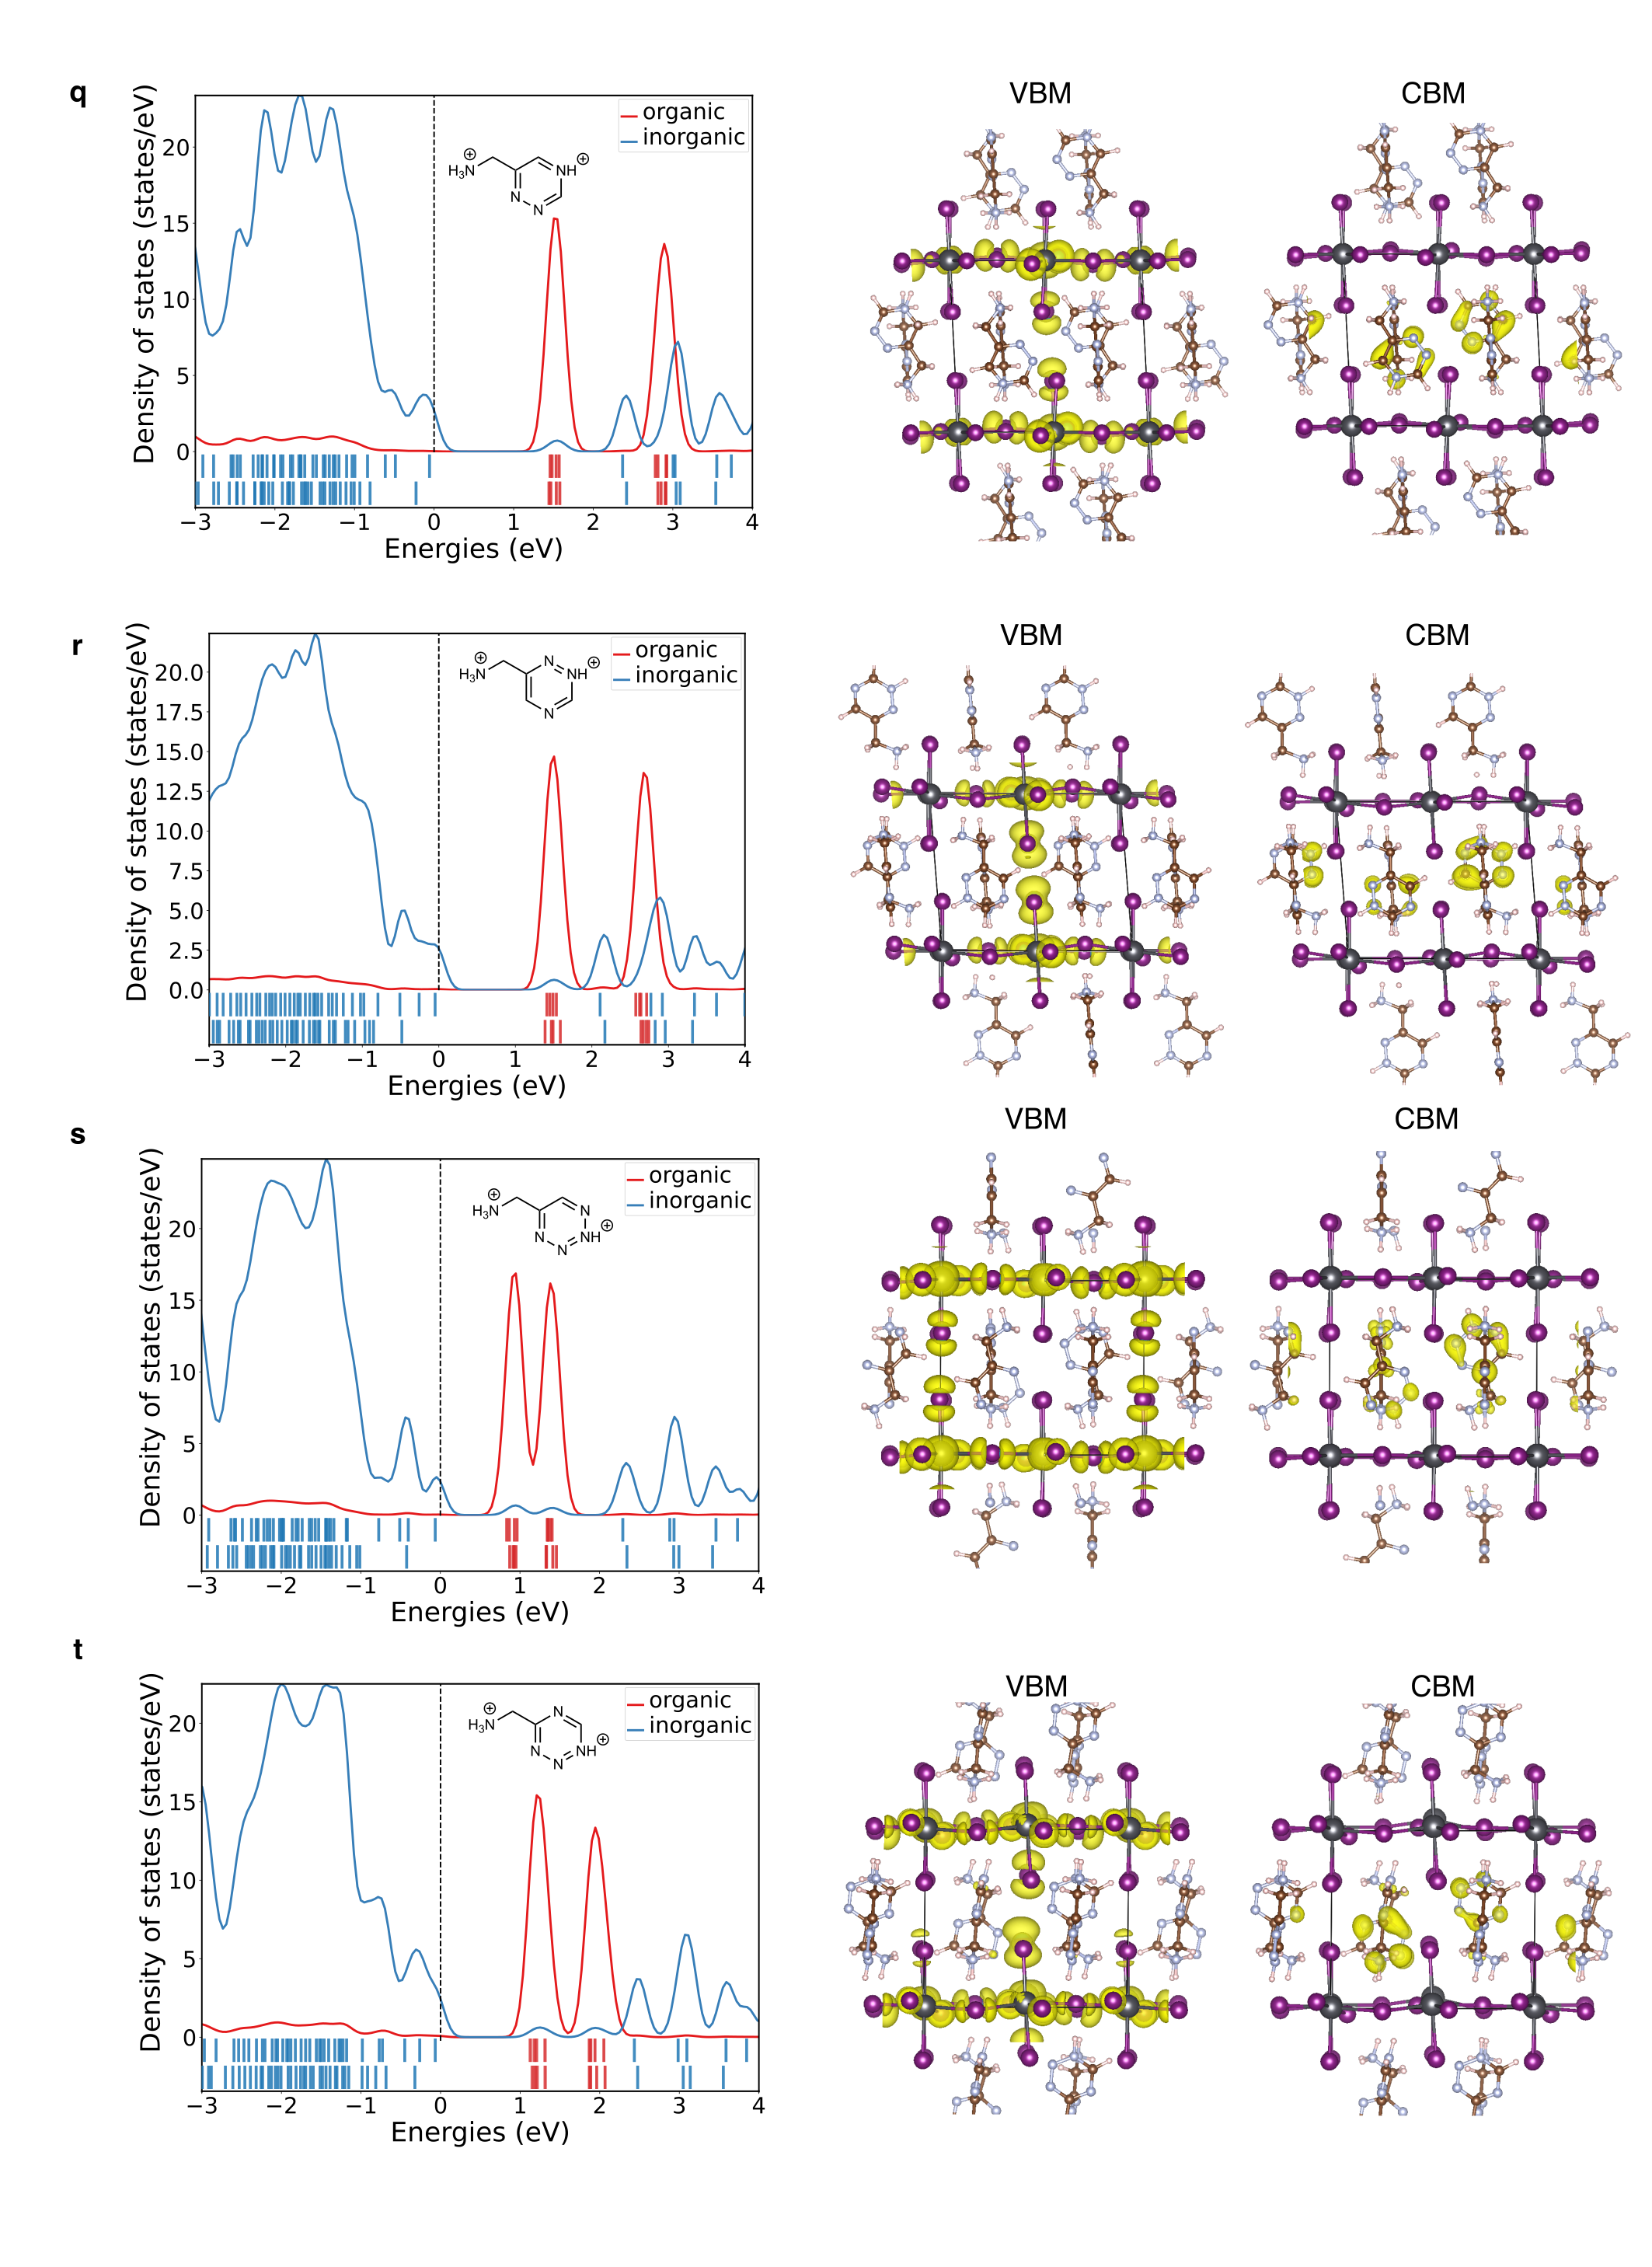
\includegraphics[width=0.9\textwidth]{figures/synthesis-feasibility/figure5-25-5.png}
    \caption{Electronic structure of inverse-designed type IIb DJ perovskites (Part 5, continued).}
\end{figure}

\begin{figure}[htbp]
    \ContinuedFloat
    \centering
    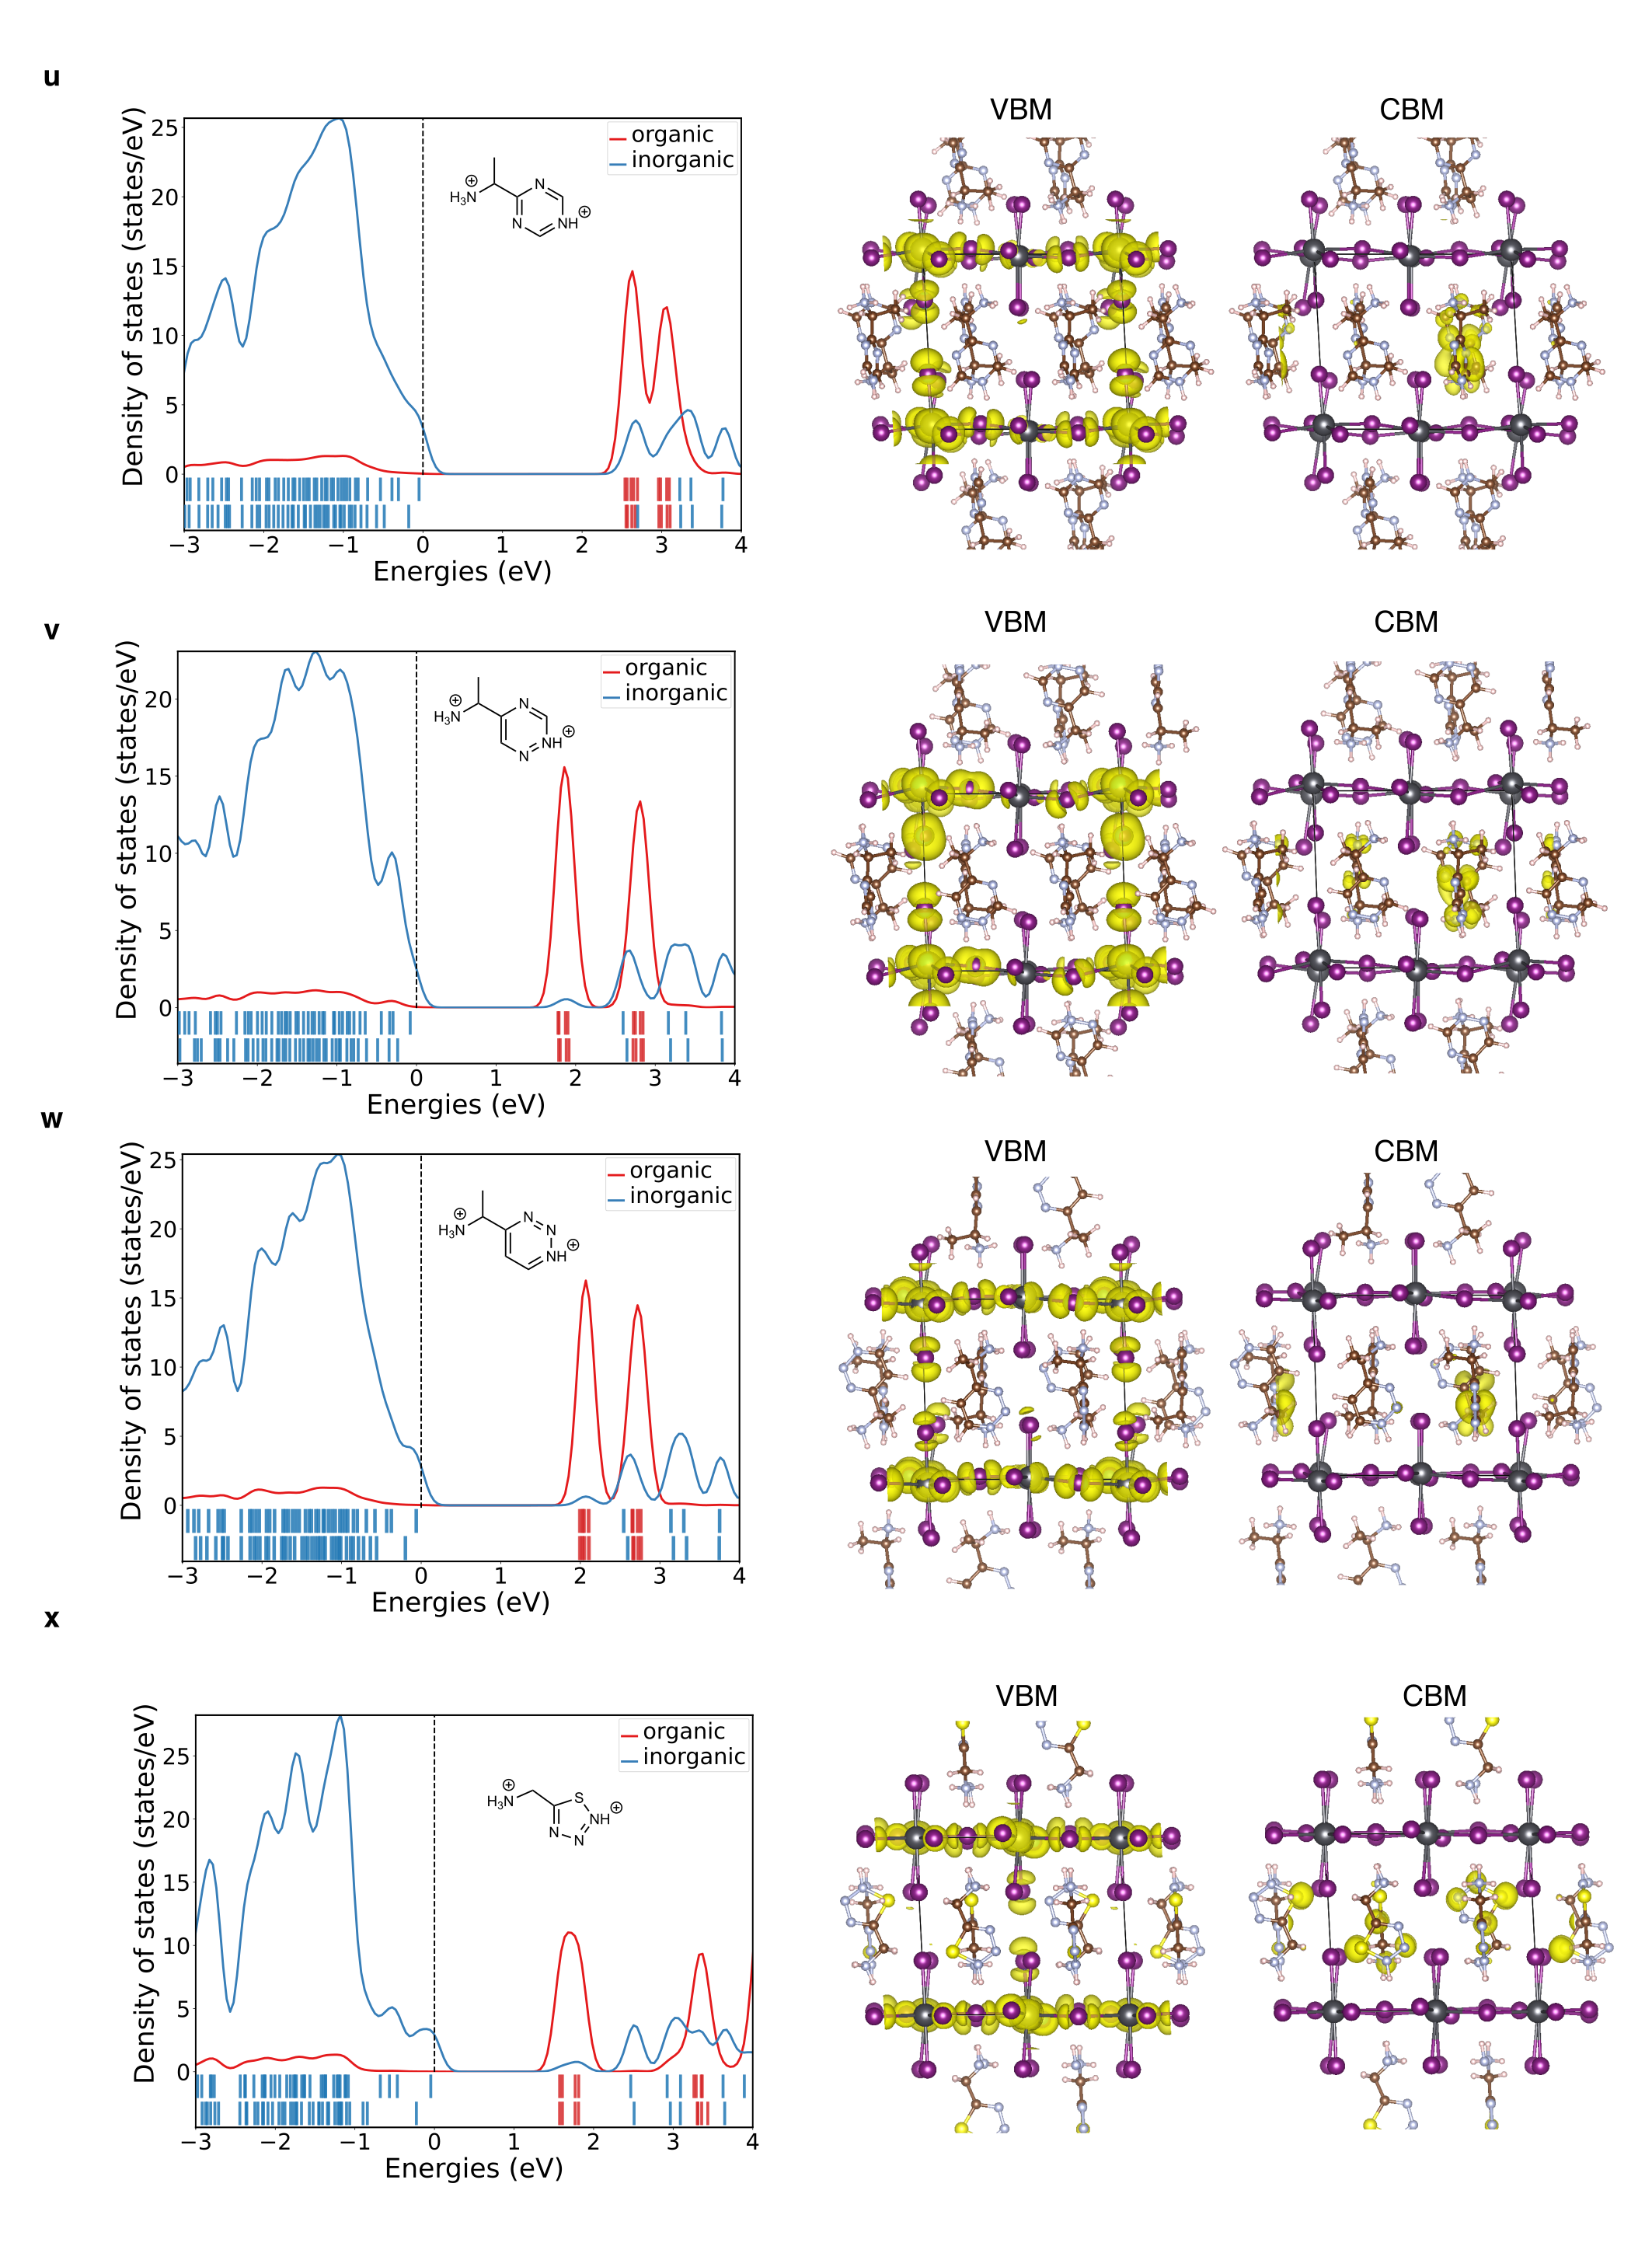
\includegraphics[width=0.9\textwidth]{figures/synthesis-feasibility/figure5-25-6.png}
    \caption{Electronic structure of inverse-designed type IIb DJ perovskites (Part 6, continued).}
\end{figure}

\begin{figure}[htbp]
    \ContinuedFloat
    \centering
    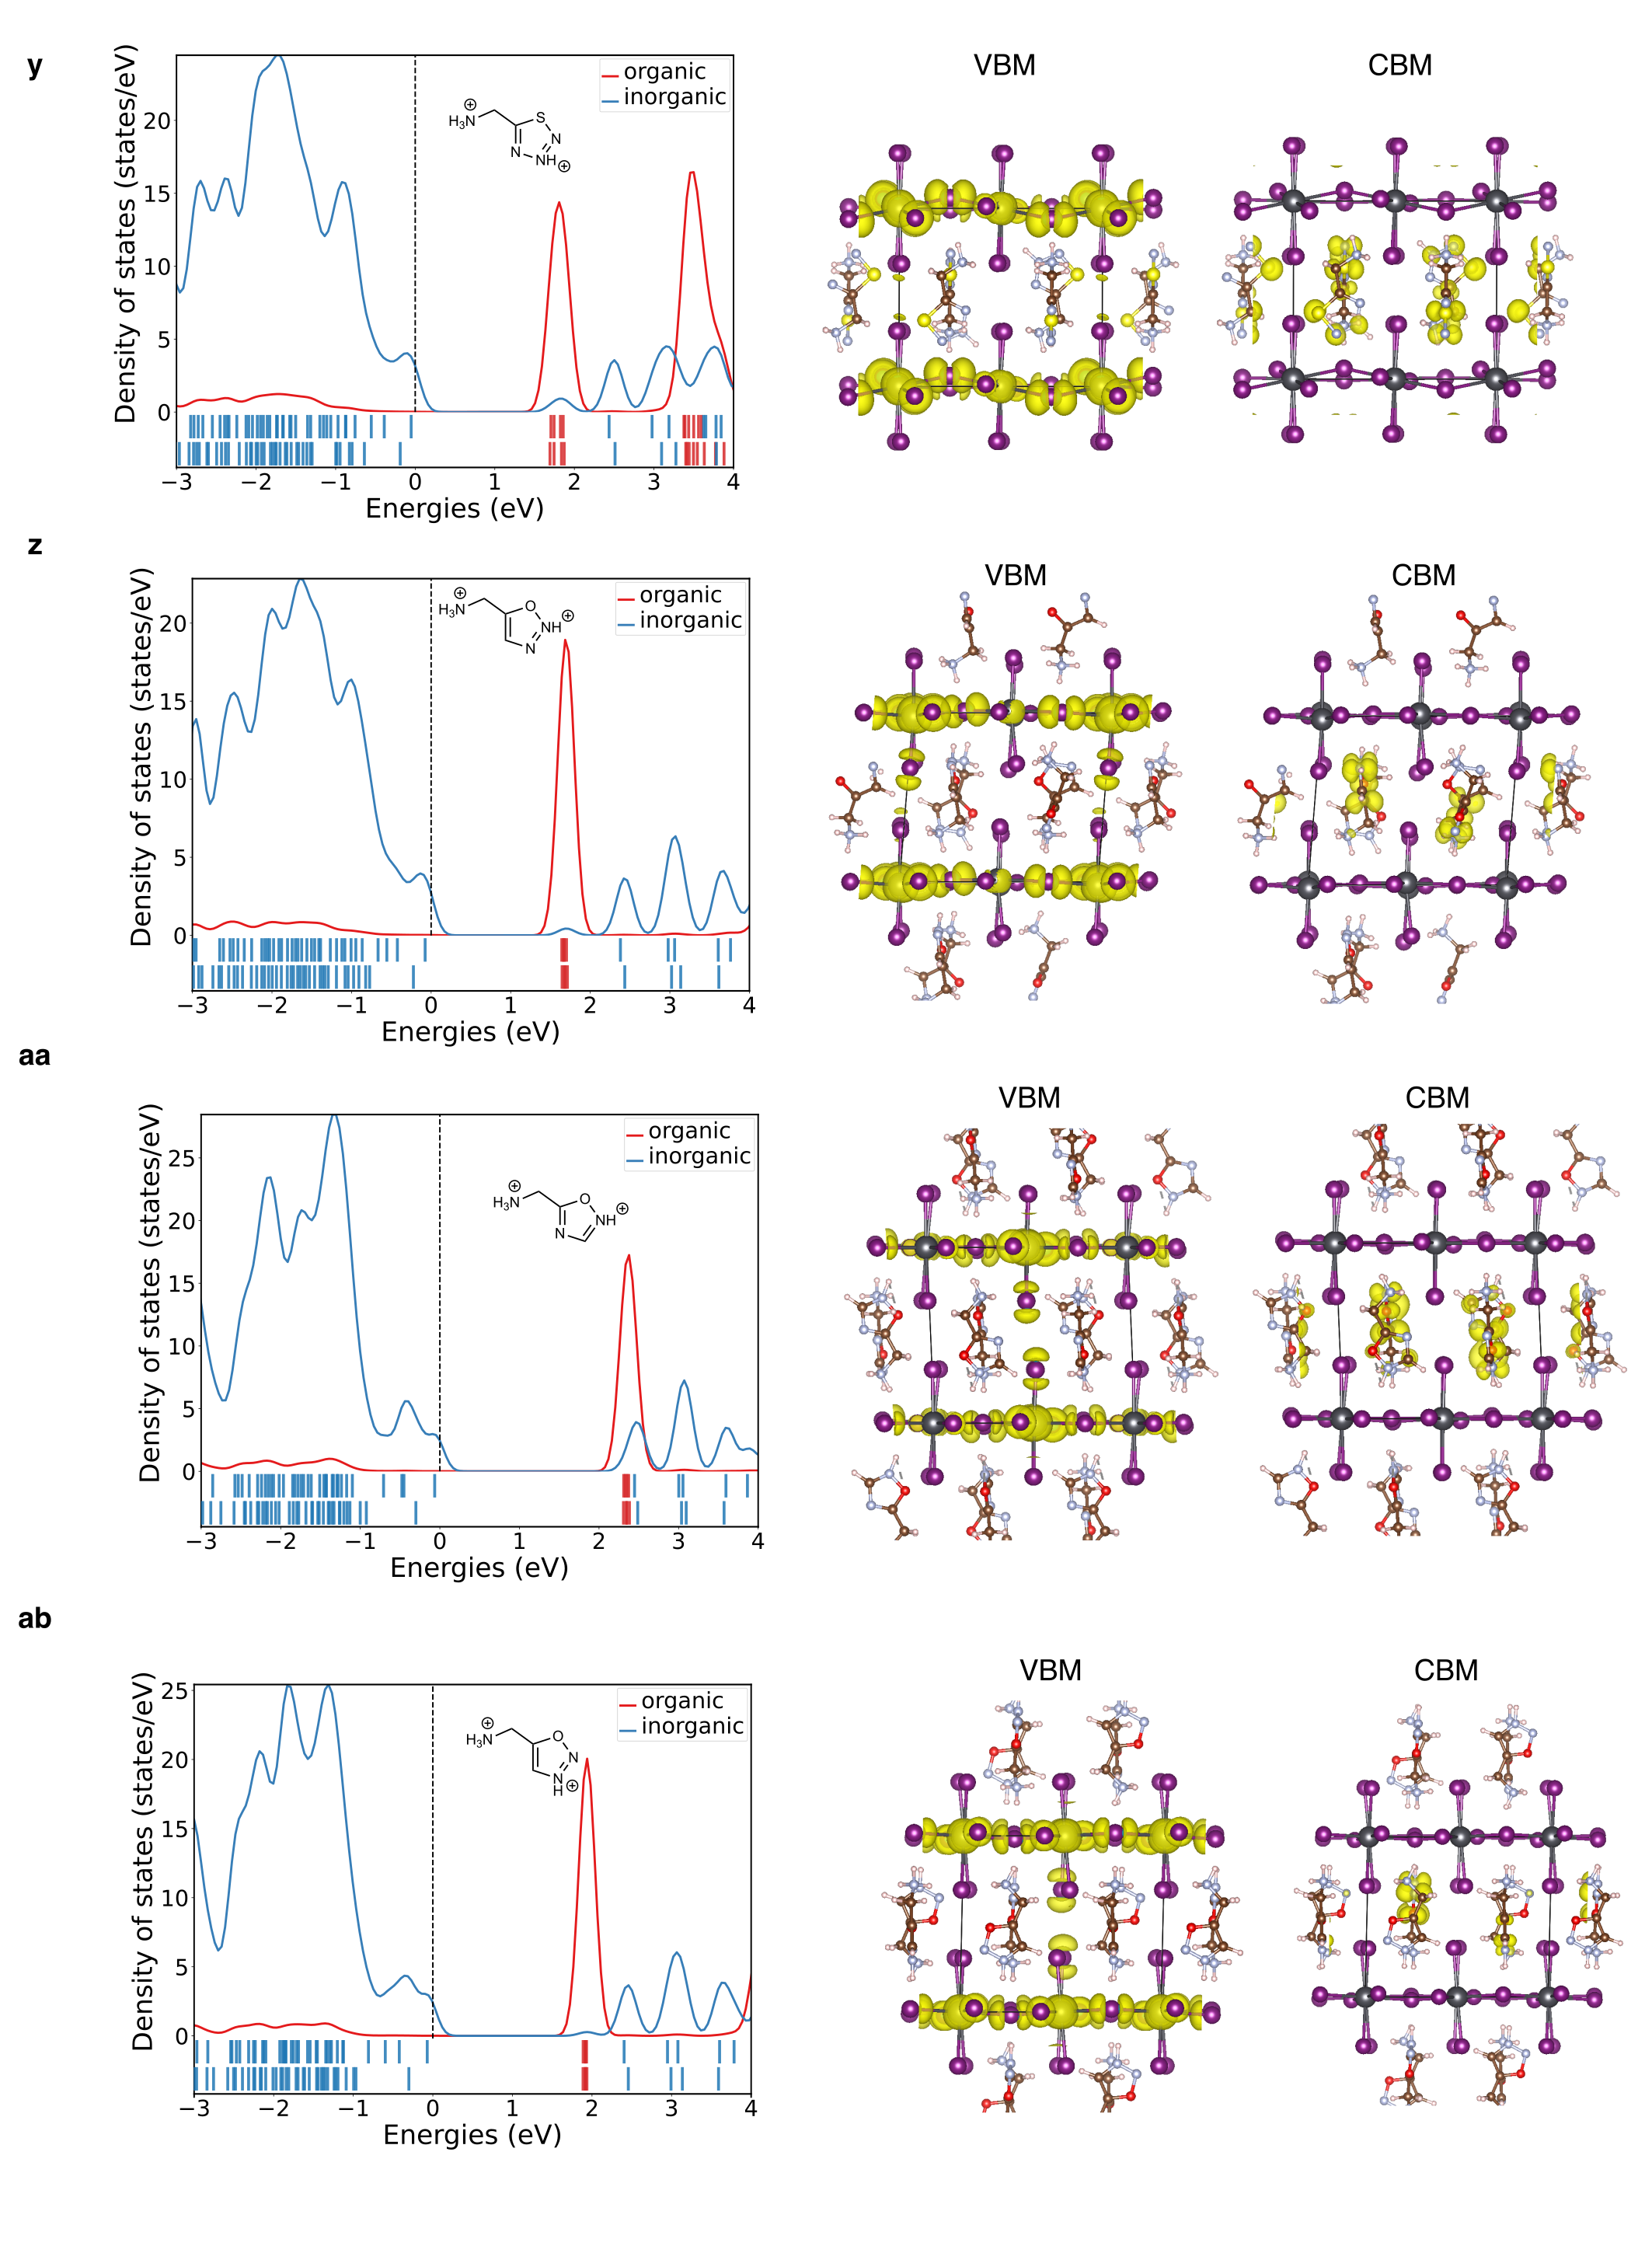
\includegraphics[width=0.9\textwidth]{figures/synthesis-feasibility/figure5-25-7.png}
    \caption{Electronic structure of inverse-designed type IIb DJ perovskites (Part 7, continued).}
\end{figure}

\begin{figure}[htbp]
    \ContinuedFloat
    \centering
    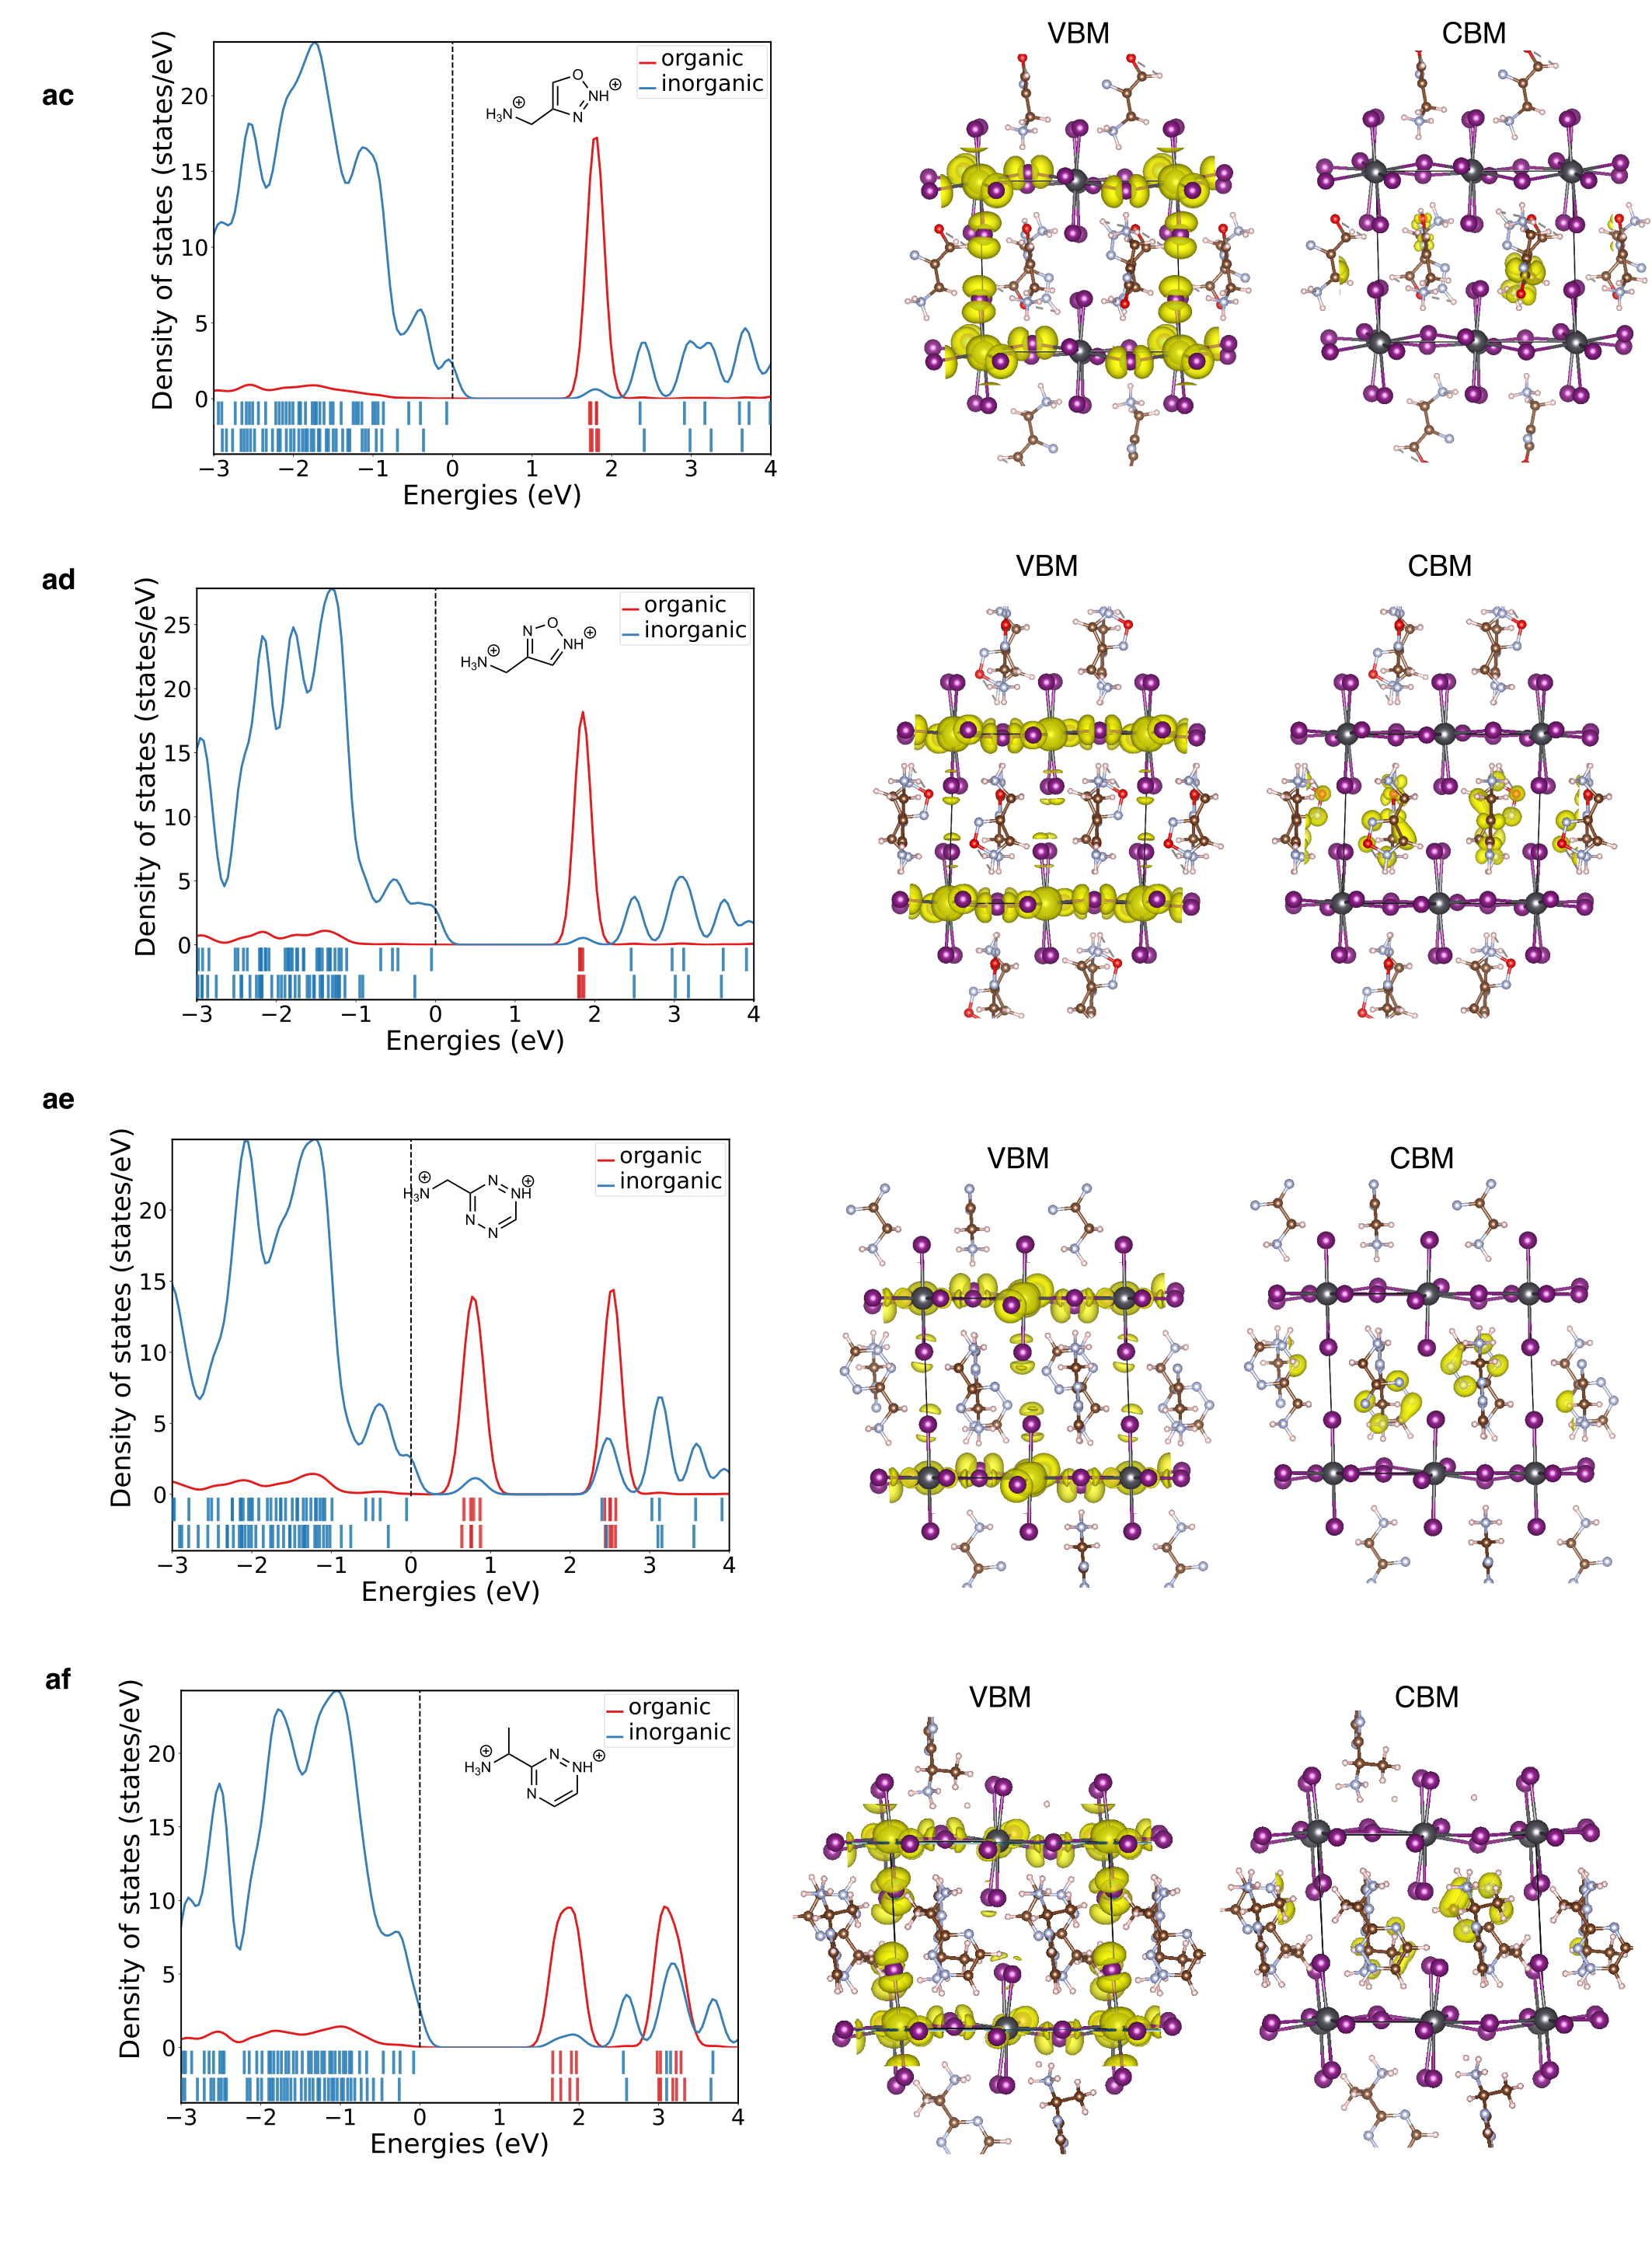
\includegraphics[width=0.9\textwidth]{figures/synthesis-feasibility/figure5-25-8.png}
    \caption{Electronic structure of inverse-designed type IIb DJ perovskites (Part 8, continued).}
\end{figure}

\begin{figure}[htbp]
    \ContinuedFloat
    \centering
    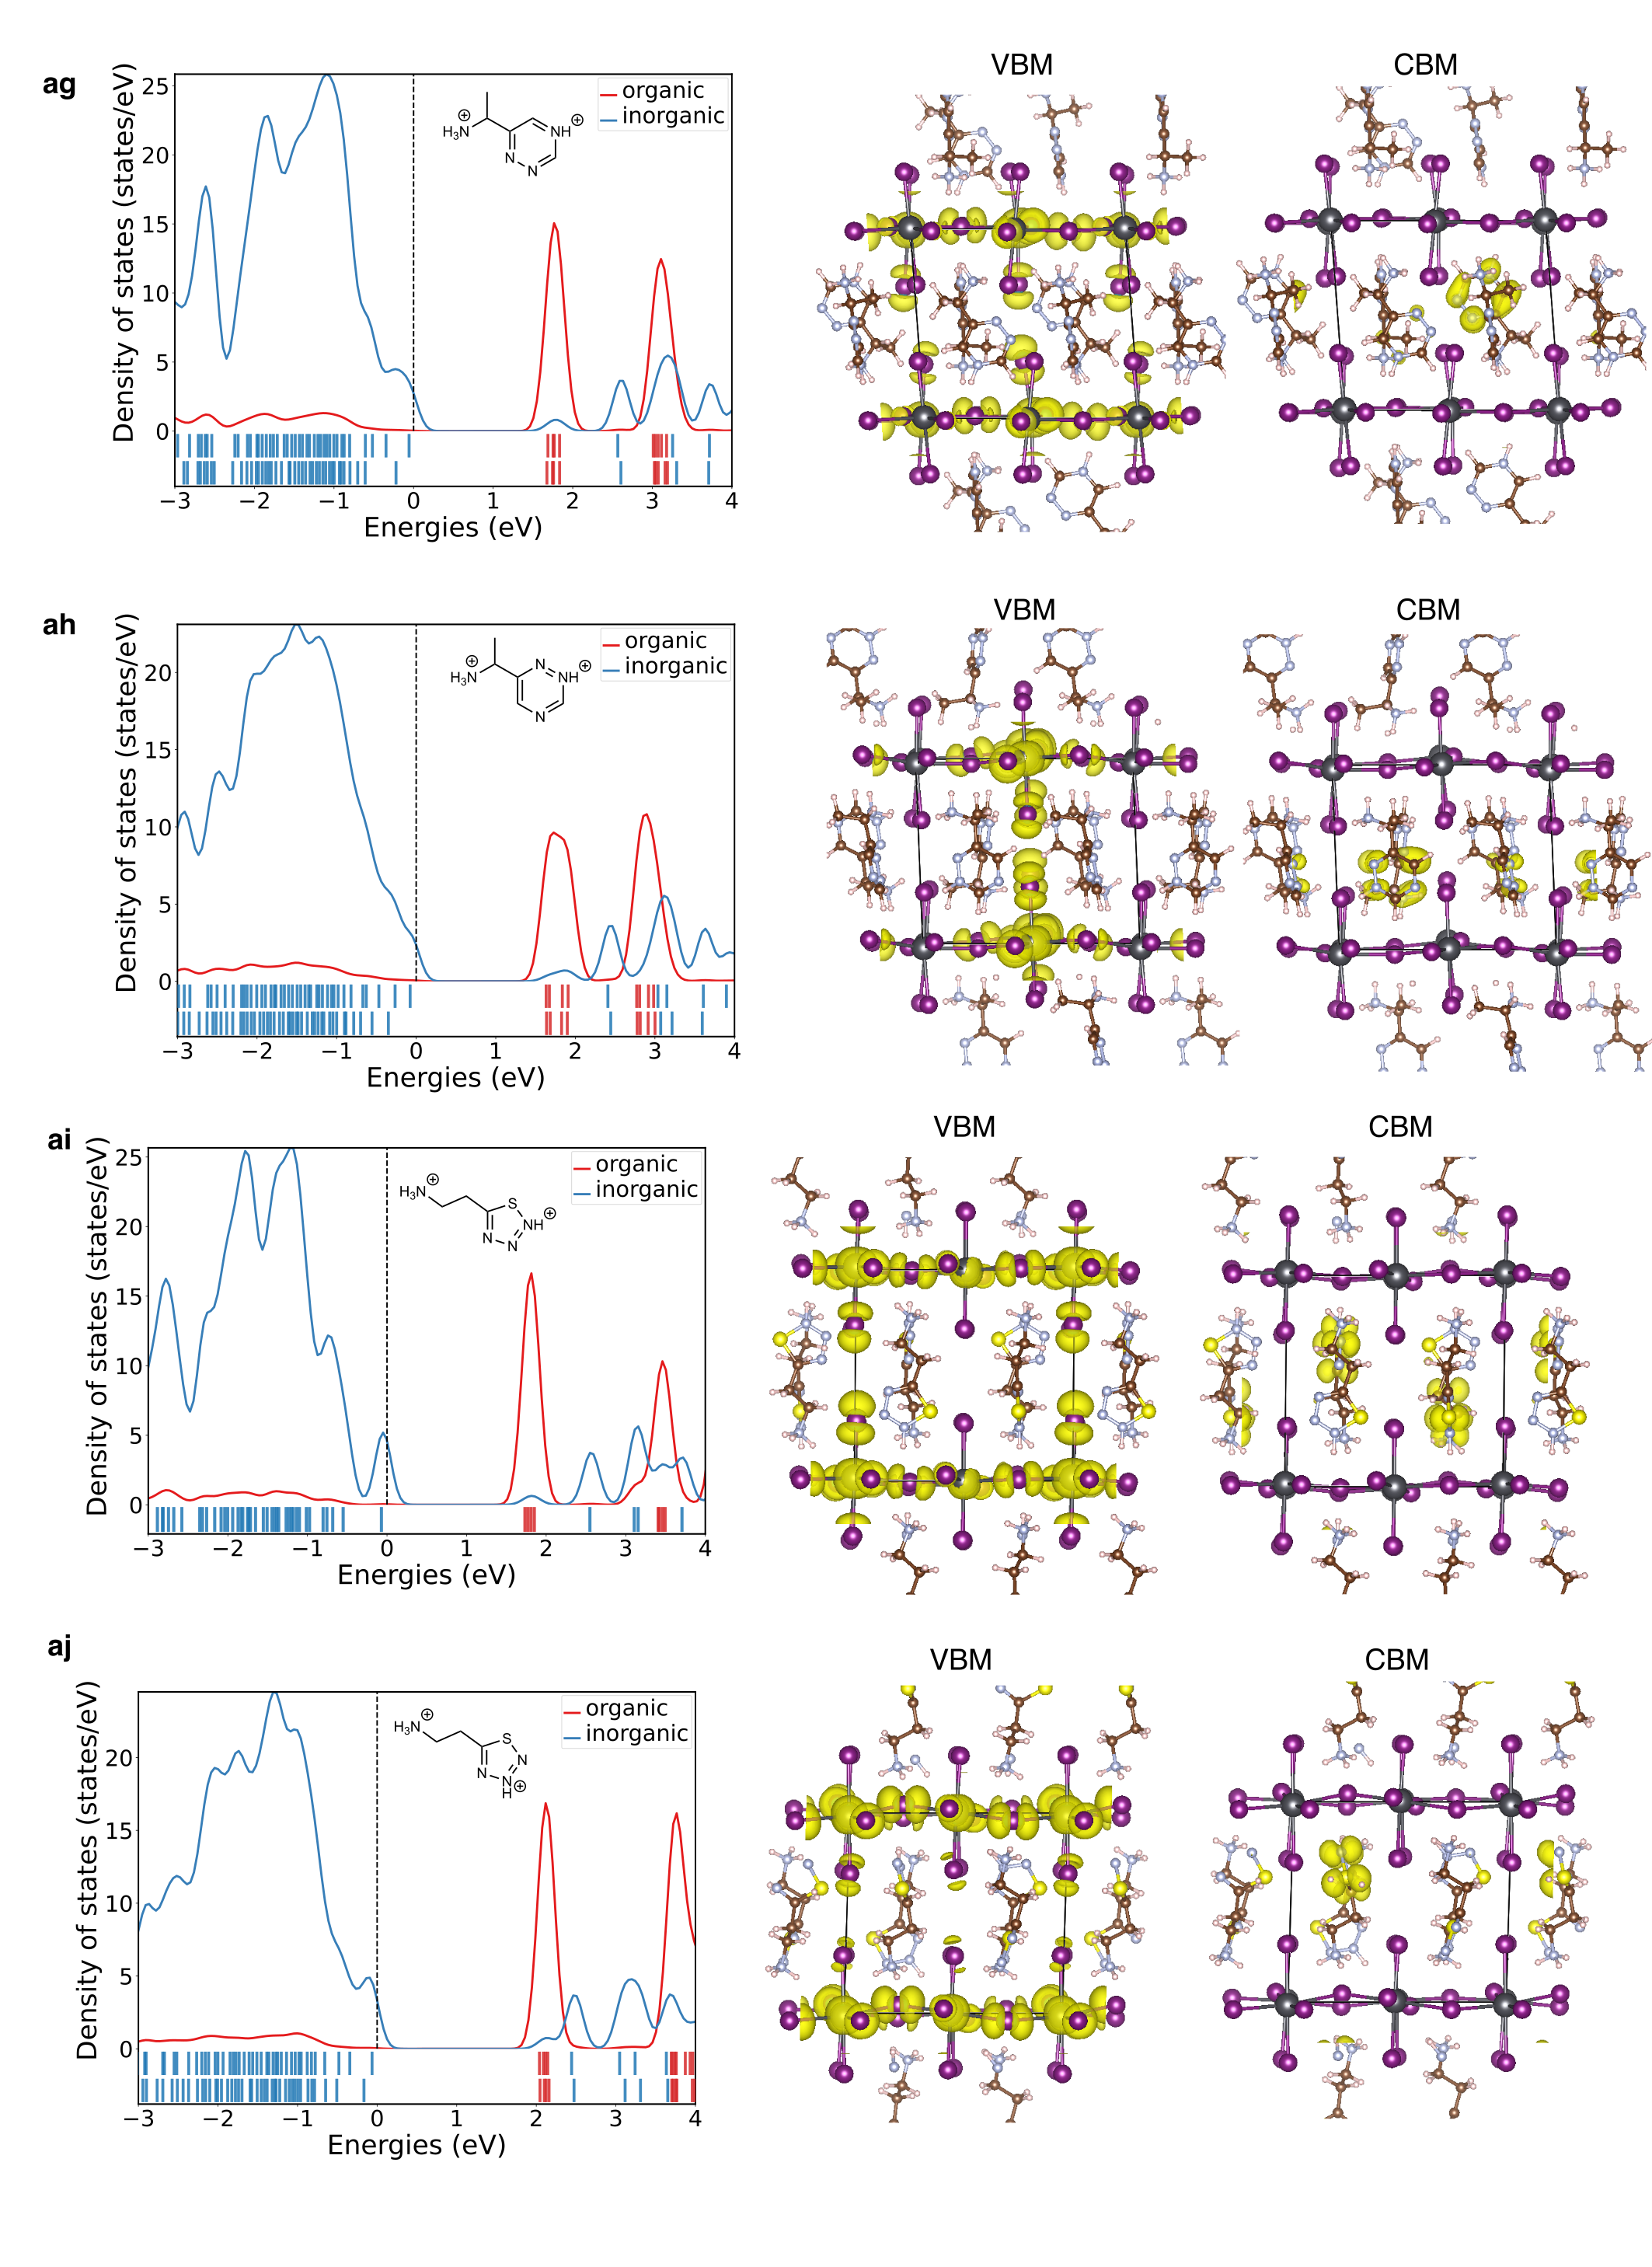
\includegraphics[width=0.9\textwidth]{figures/synthesis-feasibility/figure5-25-9.png}
    \caption{Electronic structure of inverse-designed type IIb DJ perovskites (Part 9, continued).}
\end{figure}

\begin{figure}[htbp]
    \ContinuedFloat
    \centering
    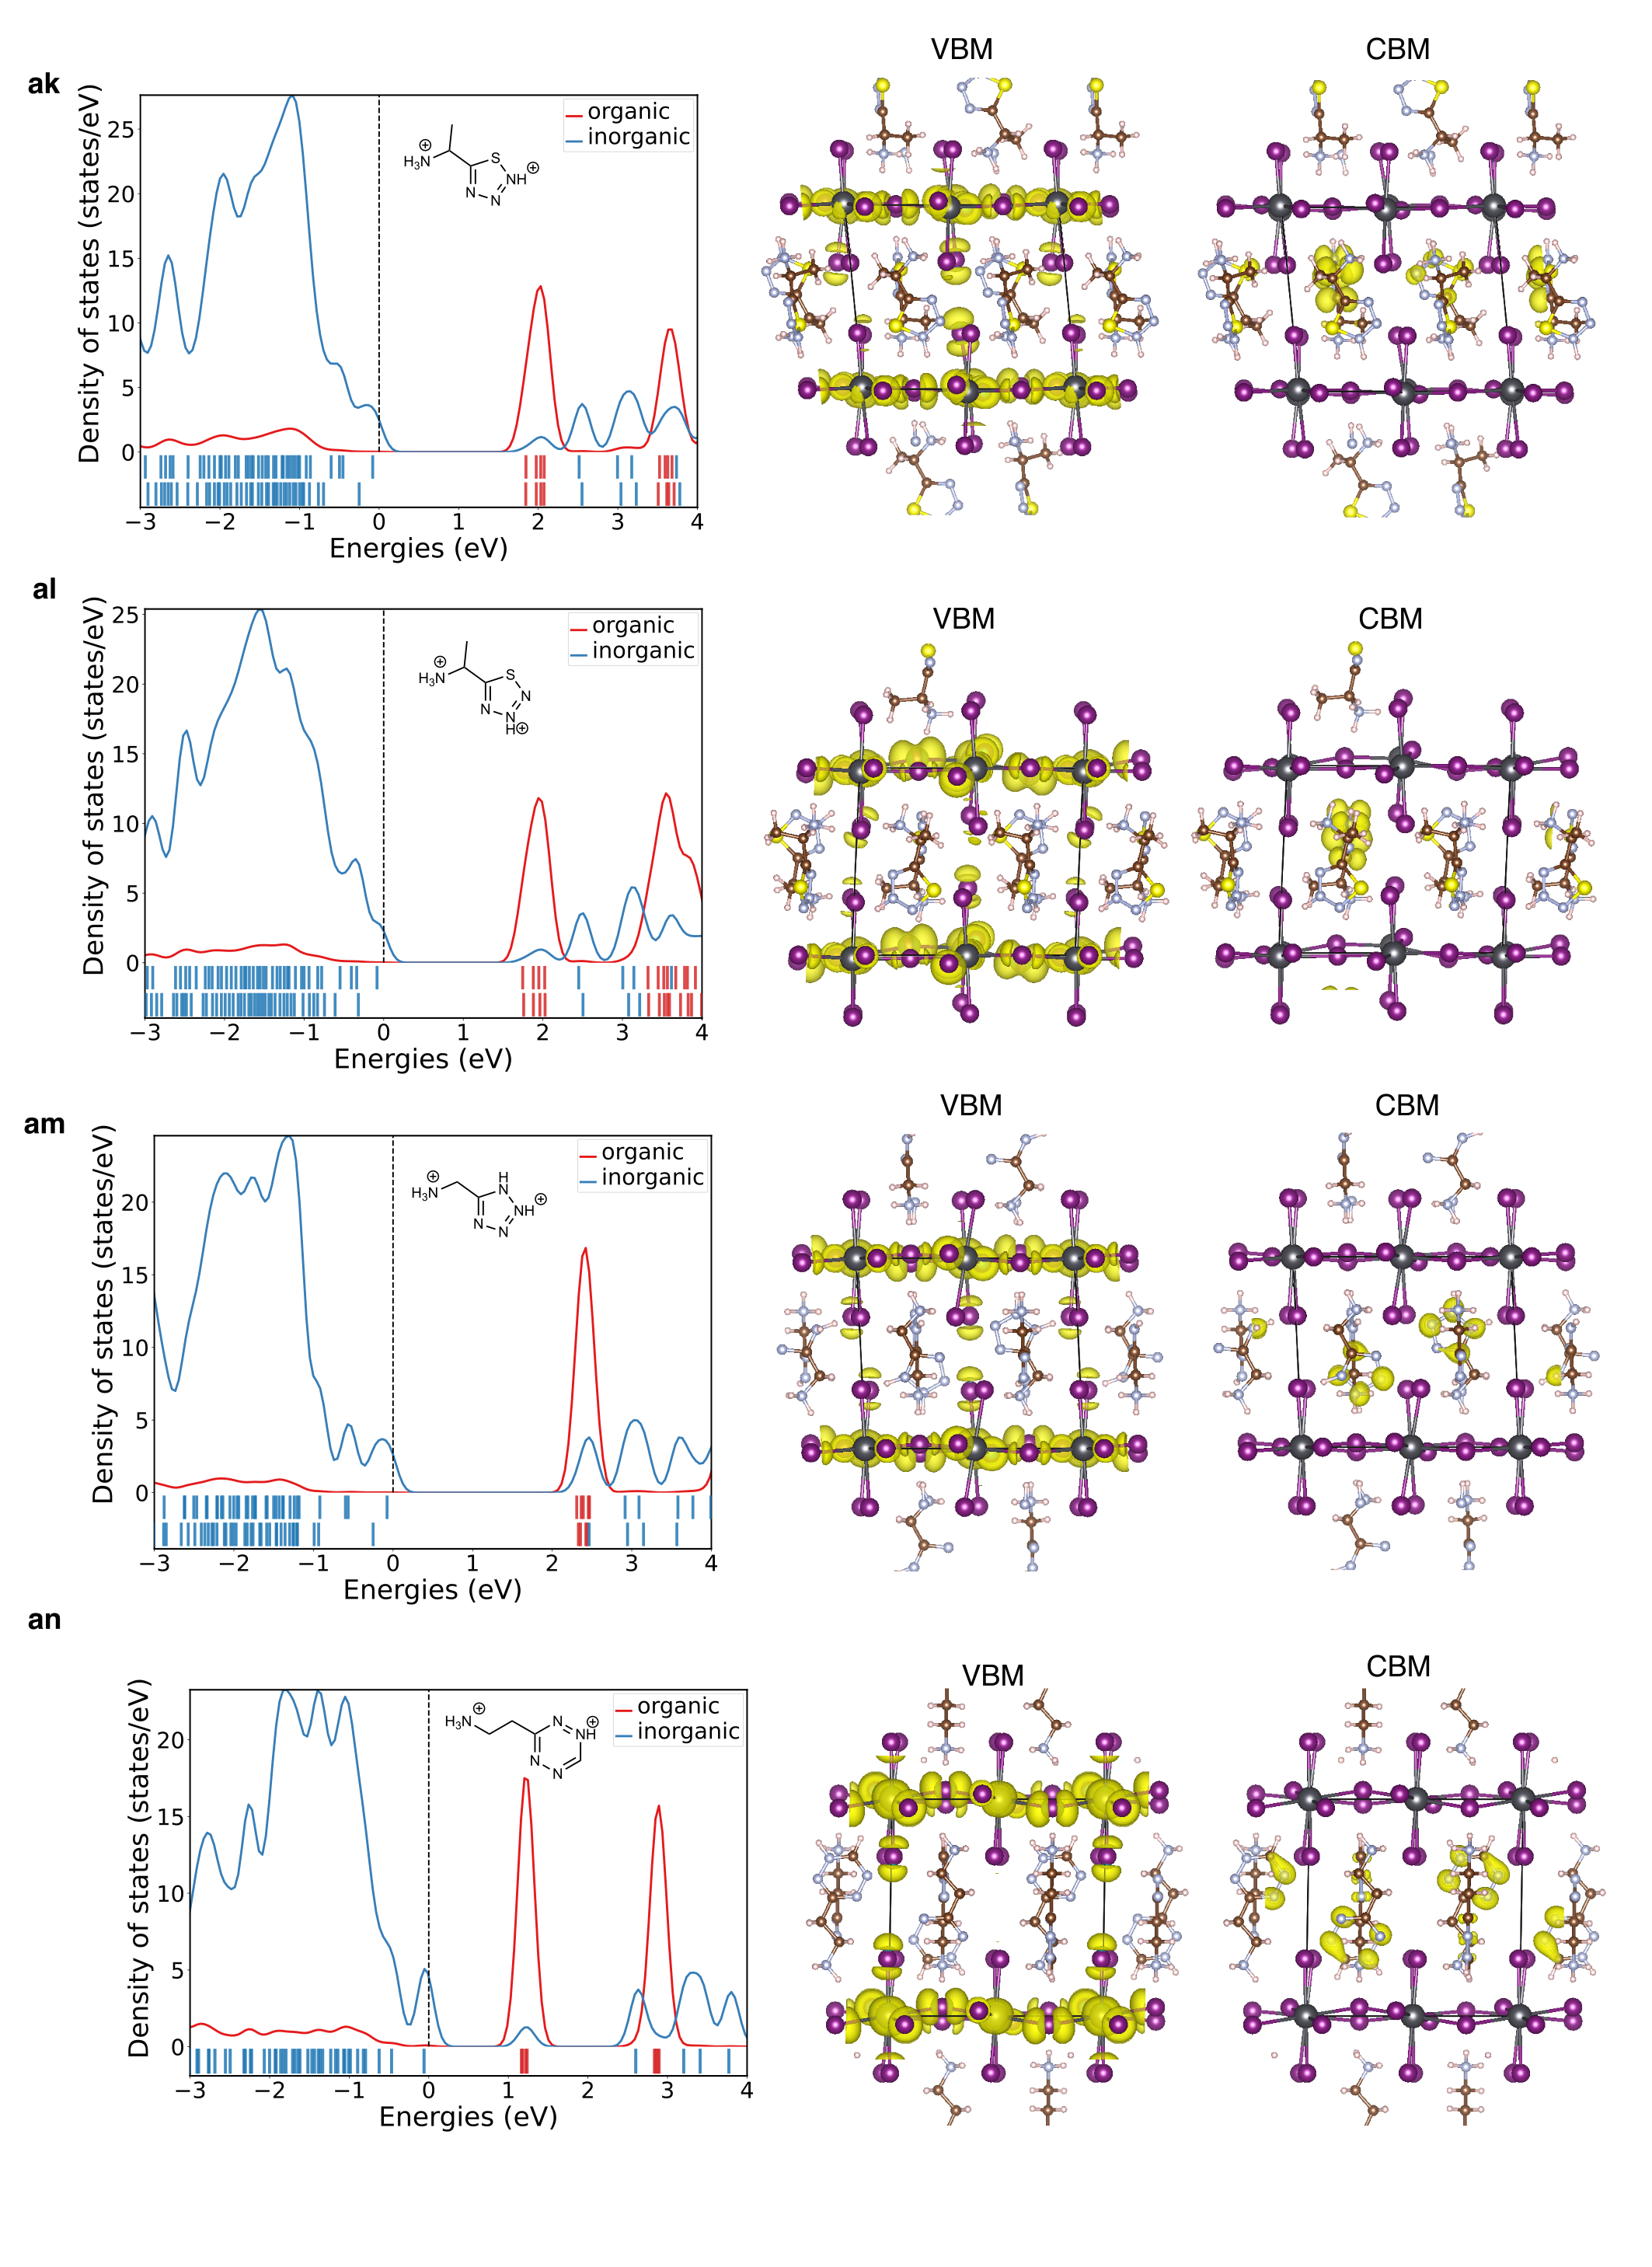
\includegraphics[width=0.9\textwidth]{figures/synthesis-feasibility/figure5-25-10.png}
    \caption{Electronic structure of inverse-designed type IIb DJ perovskites (Part 10, continued).}
\end{figure}

\begin{figure}[htbp]
    \ContinuedFloat
    \centering
    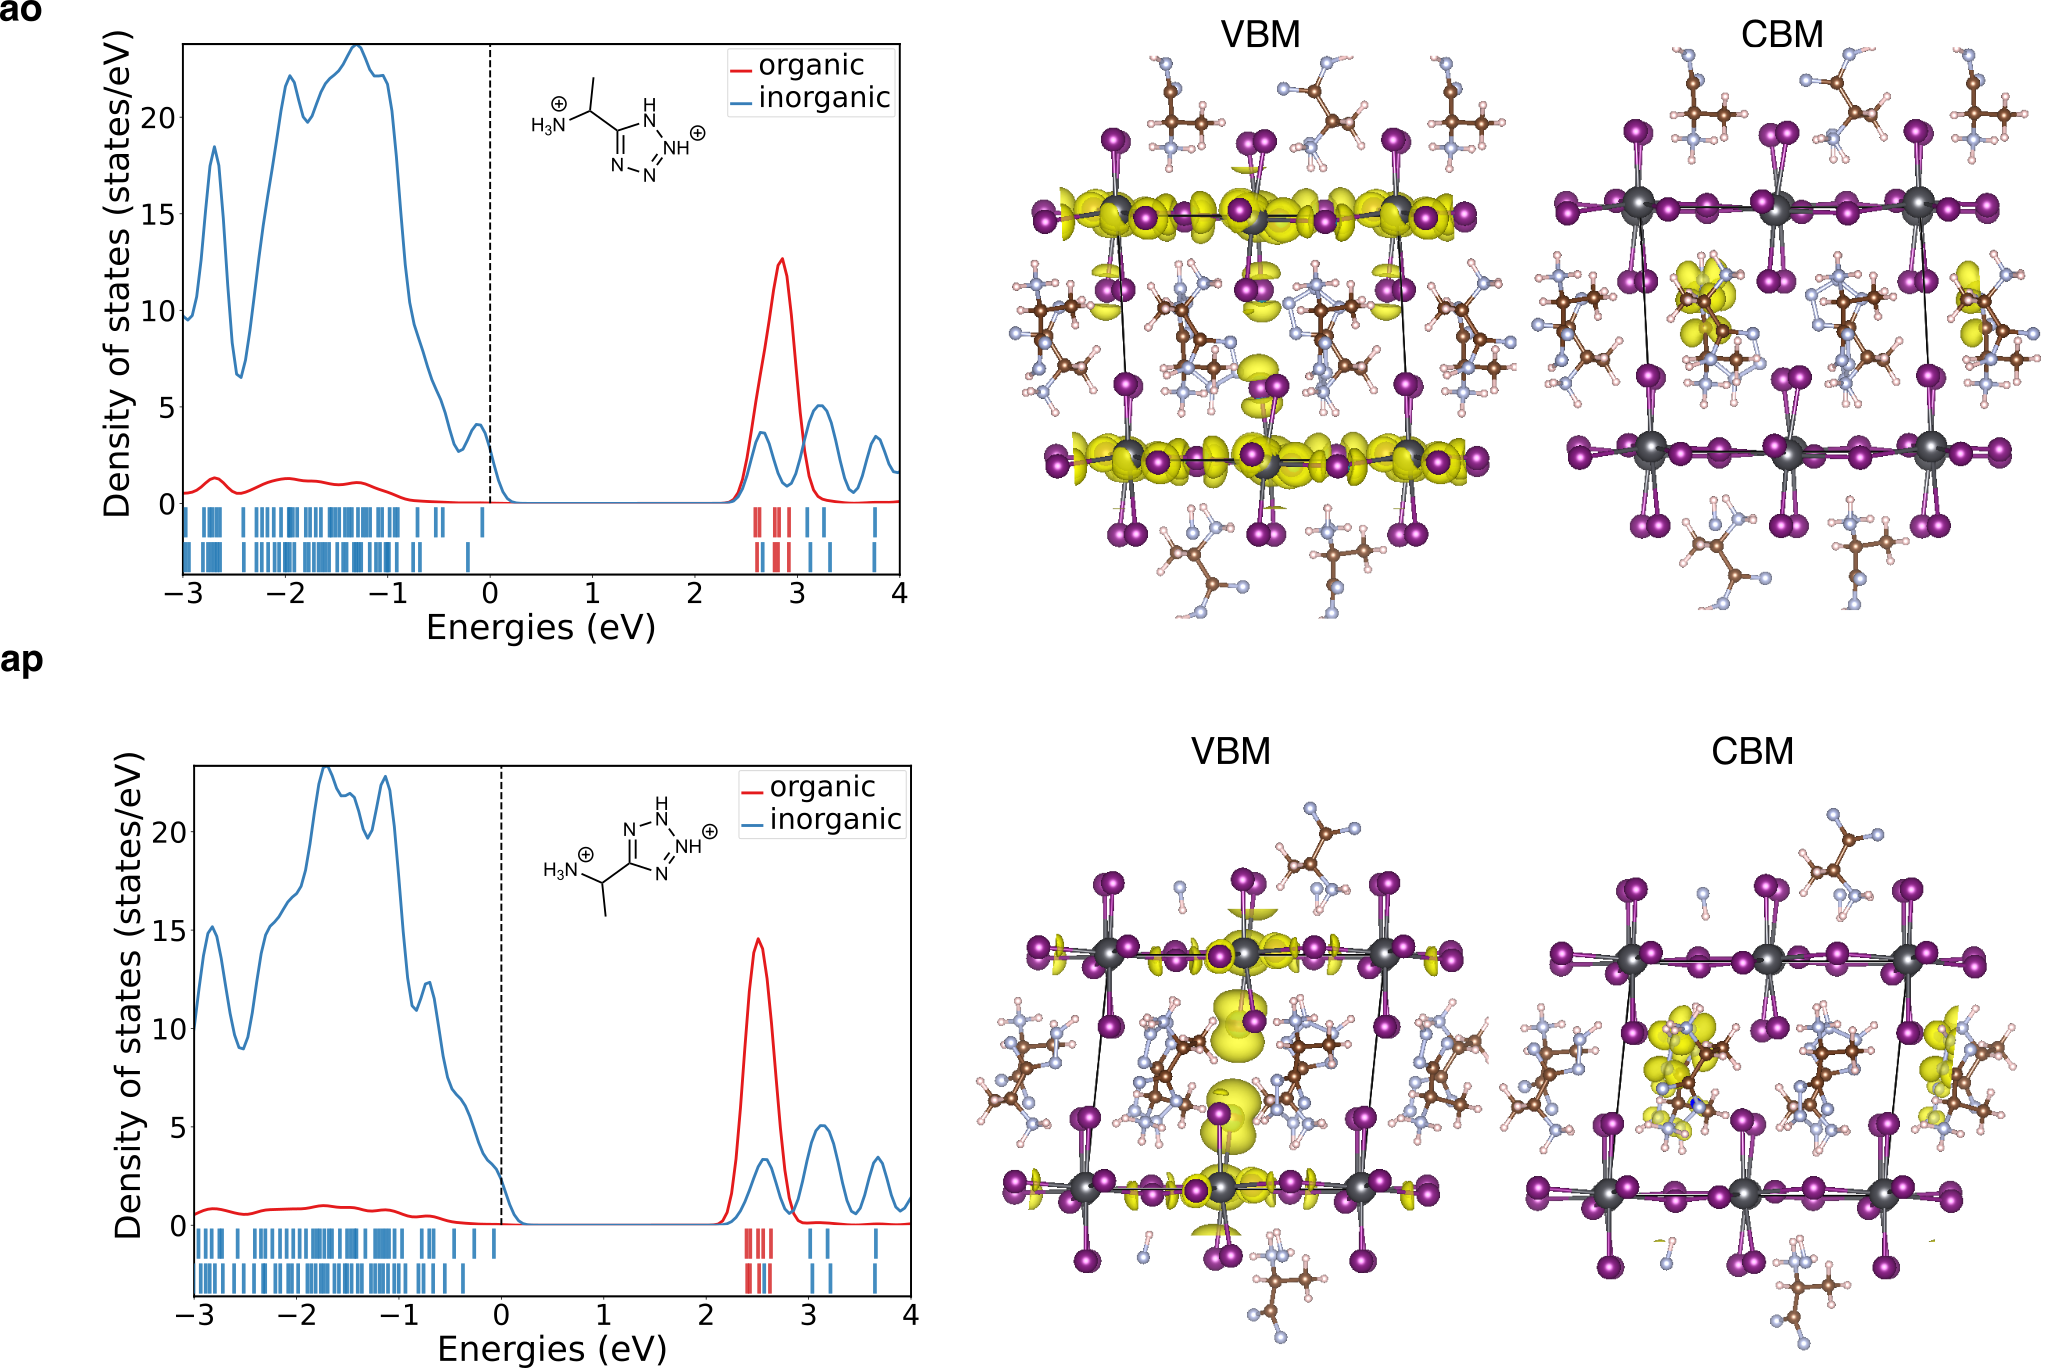
\includegraphics[width=0.9\textwidth]{figures/synthesis-feasibility/figure5-25-11.png}
    \caption{Electronic structure of inverse-designed type IIb DJ perovskites (Part 11, continued).}
\end{figure}

\clearpage
\subsection{Chemical space visualization of final candidates}

\begin{figure}[htbp]
    \centering
    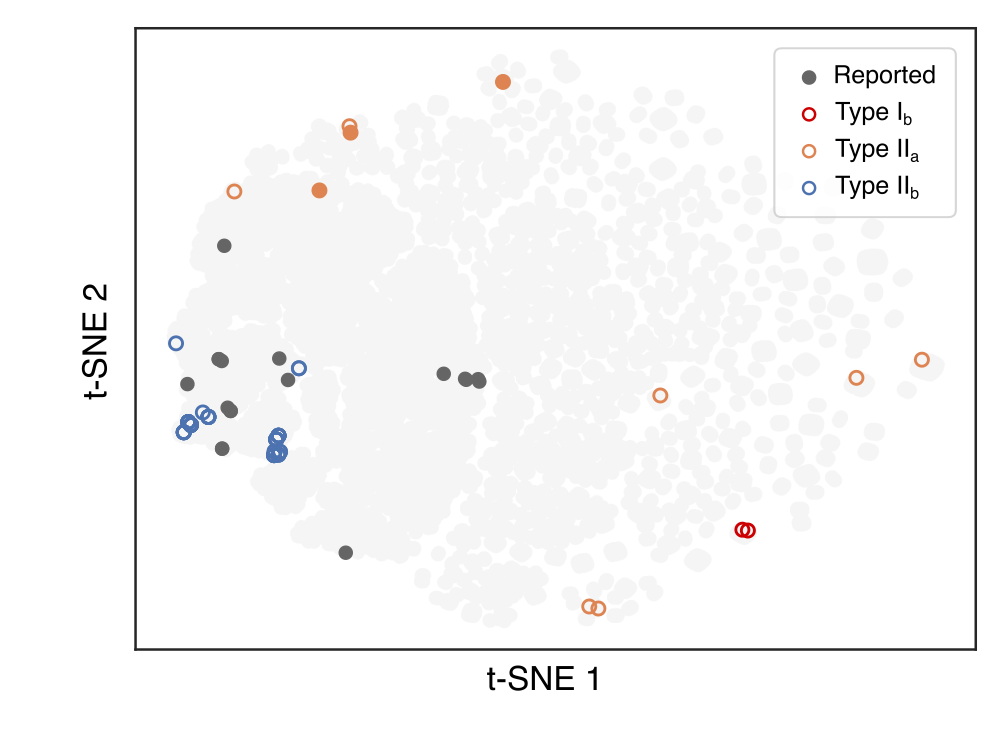
\includegraphics[width=0.9\textwidth]{figures/synthesis-feasibility/figure5-26.png}
    \caption{Chemical space visualization of inverse-designed DJ perovskites.}
    \label{fig:figure5.26}
\end{figure}

Figure \ref{fig:figure5.26} presents a t-SNE projection of the chemical space defined by the 12-digit fingerprint, highlighting both experimentally reported DJ-phase organic spacers (solid circles) and newly discovered candidates (open circles) with favorable energy level alignment types: Type Ib, Type IIa, and Type IIb. The reported spacers cluster primarily in the left-central region of the map, indicating a relatively narrow exploration of the broader chemical space. This cluster is dominated by molecules with a single aromatic ring and short linker lengths. In contrast, the newly discovered candidates—identified through inverse design and machine learning—are more broadly distributed, often occupying regions sparsely populated or entirely unoccupied by known compounds.

Type Ib candidates are located predominantly in the bottom-right region, far from the known spacers. These molecules tend to have five-membered rings and relatively short linkers. Type IIa candidates are more widely spread, including both known structures near the top of the map and newly identified candidates in remote regions, indicating chemical diversity within this alignment category. Type IIb spacers are mostly found in the center-left region, within a moderately dense area of the chemical space, yet still occupy a subspace not covered by any reported spacers.

These observations highlight the ability of the proposed workflow to identify chemically distinct and previously unexplored candidates. The clear spatial separation between known and newly designed molecules reinforces the novelty of the final candidates and supports the claim that this data-driven approach effectively expands the chemically relevant design space for DJ-phase perovskites.




\section{Chapter summary}

This chapter addressed the critical challenge of bridging computational predictions with experimental feasibility in 2D perovskite design. A two-step screening strategy was introduced to assess the synthetic accessibility of candidate organic spacers, incorporating cheminformatics-based filtering and literature cross-referencing. This was followed by the inverse design of final DJ-phase candidates, which balanced desired energy level alignment with practical constraints. The resulting shortlist of spacers represents a set of experimentally viable materials with targeted electronic properties, laying the groundwork for future experimental validation.
